\chapter{Sidechains}\label{chapter:sidechains}

\todo{Re-read this chapter and clean up}

We now have all the required tools and primitives to build sidechains. In this chapter we construct full blockchain interoperability.
We begin in Section~\ref{section:sidechains:stake} by giving the definition of what sidechains are and a construction for stake-based blockchains first, making use of the ATMS primitive defined and constructed in Chapter~\ref{chapter:stake}.
In Section~\ref{section:sidechains:work} we show how one can construct sidechains for work-based blockchains using the NIPoPoWs primitive which was discussed in Chapter~\ref{chapter:work}. These two sidechain constructions are bidirectional.
In Section~\ref{section:sidechains:burn} we explore how money can be destroyed on one system and re-created in another, giving rise to unidirectional sidechains.

% stake
\section{Bidirectional Sidechains with Stake Sources}\label{section:sidechains:stake}
In this section we give the first formal definition of security desiderata for
a system of pegged ledgers (popularly often called sidechains).
We start by conveying its intuition and then proceed to the formal treatment. We will first present a generic framework defining sidechain security upon which we will build a solution for stake-based blockchains. In the later sections of this chapter, we will explore how this can be instantiated for proof-of-work.

To prove any meaningful security
guarantees for the executed protocol without further restrictions (as it, for
example, does not prevent the adversary from corrupting all the participating
parties), we will consider such additional
assumptions, and will only
provide security guarantees as long as such assumptions are satisfied.
These assumptions will be specific to the protocol in consideration, and will be an
explicit part of our statements.\footnote{As an example, we will be assuming that a
majority of a certain pool of stake is controlled by uncorrupted parties.}

Without loss of generality, we give a detailed presentation of our construction on a generic PoS protocol
 based on Ouroboros PoS~\cite{ouroboros} (see Chapter~\ref{chapter:background} for an overview of Ouroboros). We give an overview of our construction for other proof-of-stake schemes in Section~\ref{section:other}, in particular for Ouroboros
Praos~\cite{praos}, Ouroboros Genesis~\cite{genesis}, Snow
White~\cite{snowwhite}, and Algorand~\cite{algorand}.

In this section, we formalize the notion of sidechains by proposing a rigorous
cryptographic definition, the first one to the best of our knowledge. The
definition is abstract enough to be able to capture the security for blockchains
based on proof-of-work, proof-of-stake, and other consensus mechanisms.

A critical security feature of a  sidechain system that we formalise
is the \textit{firewall property} in
which a catastrophic failure in one of the chains, such as a violation of its
security assumptions, does not make the other chains vulnerable providing a
sense of limited liability.%
\footnote{To follow the analogy with the term of limited liability in corporate
law, a catastrophic sidechain failure is akin to a corporation going bankrupt
and unable to pay its debtors. In a similar fashion, a sidechain in which the
security assumptions are violated may not be able to cover all of its debtors.
%In fact,
%because it can be under attack,
We give no assurances regarding assets residing on a sidechain if its
security assumptions are broken.
 However, in the same way that stakeholders of a corporation are personally
protected in case of corporate bankruptcy, the mainchain is also protected in
case of sidechain security failures. Our security will guarantee that
each incoming transaction from a sidechain will always have a valid
explanation  in the sidechain ledger
independently of whether the underlying
security assumptions are violated or not. A simple embodiment of this rule
is that a sidechain can return to the mainchain at most as many coins as they have been sent to the sidechain over all time.
}
The   firewall property formalises and generalises the concept of a blockchain \textit{firewall} which was described in high level in~\cite{sidechains}. Informally the blockchain firewall suggests
that no more money can ever return from the sidechain than the amount that was moved
into it. Our general firewall property  allows relying on an
arbitrary definition of exactly how assets can correctly be moved back and forth
between the two chains, we capture this by a so-called
\textit{validity language}. In case of failure, the firewall
ensures that transfers from the sidechain into the mainchain are rejected unless
there exists a (not necessarily unique) plausible history of events on the sidechain that could, in case the
sidechain was still secure, cause the particular transfers to take place.
%If
%the correctness validity language describing the valid transfers between the
%mainchain and the sidechain consists of a simple law of conservation, then the
%limited liability  property captures  precisely a blockchain firewall.

In this section, we outline a concrete exemplary
construction for sidechains for proof-of-stake
blockchains. For conciseness our construction is described
with respect to a generic PoS blockchain consistent with the  Ouroboros
protocol~\cite{ouroboros} that underlies the Cardano blockchain, which is currently one of the largest
pure PoS blockchains by market capitalisation,\footnote{See \url{https://coinmarketcap.com}. }
nevertheless we also discuss how to modify our construction to
operate for
Ouroboros Praos~\cite{praos},
Ouroboros Genesis~\cite{genesis},
Snow White \cite{snowwhite}
and
Algorand \cite{algorand}.

We prove our construction secure   using standard cryptographic
assumptions. We show that our construction (i) supports safe cross-chain value
transfers when the security assumptions of both chains are satisfied, namely
that a majority of honest stake exists in both chains, and (ii) in case of a
one-sided failure,  maintains the firewall property, thus
containing the damage
to the chains whose security conditions have been violated.
%

A critical consideration in a sidechain construction is safeguarding
a new sidechain in its initial ``bootstrapping'' stage against a ``goldfinger'' type of attack \cite{mining-economics,hostile}. Our construction
features a mechanism we call {\em merged-staking}
that allows  mainchain stakeholders who have signalled
sidechain awareness to create sidechain blocks even without moving stake
to the sidechain. In this way, sidechain security can be maintained
assuming honest stake majority among the entities that have signaled sidechain
awareness that, especially in the bootstrapping stage, are expected to be
a large superset of the set of stakeholders that maintain assets
in the sidechain.
%Refel the maintainers
%of the sidechain need to monitor the blocks generated by the mainchain, but the
%maintainers of the mainchain need not be aware of the sidechain's blocks.

Our techniques can be used to facilitate various forms of 2-way peggings
between two chains. As an illustrative example we focus on a parent-child
mainchain-sidechain
configuration where sidechain nodes follow also the mainchain (what we call direct observation) while mainchain nodes need to be able to receive cryptographically
certified signals
from the sidechain maintainers,
taking advantage of the proof-of-stake nature of the underlying protocol. This is achieved by having
mainchain nodes maintain sufficient information about the sidechain that allows
them to authenticate a
small subset of  sidechain stakeholders that is sufficient to
reliably represent the view of a stakeholder majority on the sidechain.
%a recent snapshot of the stakeholder distribution on
%the sidechain (committed in the form of a Merkle-Patricia trie)
This piece of information is updated in regular intervals to account
for  stake shifting on the sidechain.
Exploiting this, each withdrawal  transaction from the sidechain to the mainchain
is signed by this  small subset of sidechain stakeholders.
%that is sufficient to reliably represent the view of a stakeholder majority on the sidechain.
To minimise overheads we batch this authentication information and all the withdrawal transactions from
the sidechain in a single message that will be prepared once per ``epoch.'' We will
refer to this signaling  as
 {\em cross-chain certification}.

In greater detail, adopting some terminology  from \cite{ouroboros},
the sidechain certificate  is constructed by obtaining
signatures  from the set of so-called \emph{slot leaders} of the last
$\Theta(k)$ slots of the previous epoch, where $k$ is the security parameter.
Subsequently, these signatures will be combined together with all necessary
information to convince the mainchain nodes (that do not have access to the
sidechain) that the sidechain certificate is valid.

\noindent {\bf  Related work. }
Sidechains were first proposed as a high level concept in~\cite{sidechains}.
%To the best of
%our knowledge, so far  no
%formal definition of sidechain security exists, and existing constructions are not
%accompanied by formal analysis.
Notable proposed implementations of the concept are given in~\cite{drivechains,lerner}.
In these works, no formal proof of security
is provided and their performance is sometimes akin to maintaining the whole
blockchain within the sidechain, limiting any potential scalability gains.
%
There have been several attempts to create various cross-chain transfer
mechanisms including Polkadot~\cite{polkadot},
Cosmos~\cite{tendermint}, Blockstream's Liquid \cite{federated-interoperability} and Interledger \cite{interledger}. These constructions  differ in various aspects from our work including in that
they focus on proof-of-work or private (Byzantine) blockchains, require
federations, are not decentralized and --- in all cases ---
 lack a formal security model and analysis.
Threshold multi-signatures were considered before, e.g., \cite{pass-asynchronous},
without the ad-hoc characteristic we consider here.
A related primitive that has been considered as potentially useful for enabling
proof-of-work (PoW) sidechains (rather than PoS ones) is a (non-interactive) proof of
proof-of-work~\cite{popow,nipopows}; nevertheless,  these works do not give a
formal security definition for sidechains, nor provide a complete sidechain
construction. We reiterate that while we focus on  PoS, our definitions and model
are fully relevant for the PoW setting as well.

After treating stake-based sidechains, we turn to work-based sidechains in later
sections.

\subsection{Defining Security of Pegged Ledgers}
\label{sec:definition}

\todo{Clean up this section}

We consider a setting where a set of parties run a protocol maintaining $n$
ledgers $\Ledger_1,\Ledger_2, \ldots,\Ledger_n$, each of the ledgers potentially
carrying many different assets. (This protocol might of course be a combination
of subprotocols for each of the ledgers.)
%At any given time $t$, in the
%view of any given party $\party$, a ledger $\Ledger_i$ will is at state
%$\LState_i^{\party}[t]$.
For each $i\in[n]$, we denote by~$\Assum_i$ the security assumption
required by $\Ledger_i$: For example, $\Assum_i$ may denote that
there has never been a majority of hashing power (or stake in a particular
asset, on this ledger or elsewhere) under the control of the adversary; that a
particular entity (in case of a centralized ledger) was not corrupted; and so
on.  We assume that all $\Assum_i$ are \emph{monotone} in the sense that once
violated, they cannot become true again. Formally, $\Assum_i$ is a
sequence of events $\Assum_i[t]$ for each time slot $t$ that satisfy
$\lnot\Assum_i[t] \Rightarrow \lnot\Assum_i[t+1]$ for all $t$.
%monotone
%predicate (which can only go from \textit{true} to \textit{false}) evaluated on
%the whole execution of the respective ledger protocol.
%We denote by $\Secure$ the set $\setd{i}{\Assum_i\text{ is satisfied}}$ of indices
%of currently uncompromised ledgers.

There is an a priori unlimited number of (types of) assets, each asset
representing e.g. a different cryptocurrency.
For simplicity we assume that assets of the same type
are fungible, but our treatment easily covers also non-fungible assets.
We will allow specific rules of behavior for each asset (called \emph{validity
languages}), and each asset behaves
according to these rules on each of the ledgers where it is present.

We will fix an operator $\merge(\cdot)$ that
 merges a set of ledger states
$\mathcal{L}=\{\LState_1,\allowbreak \LState_2,\allowbreak \ldots,\allowbreak \LState_n\}$ into a single ledger
state  denoted by $\merge(\mathcal{L})$. We will discuss concrete instantiations
of $\merge(\cdot)$ later, for now simply assume that some canonical way of
merging all ledger states into one is given.

Informally, at any point $t$ during the execution, our security definition only
provides guarantees to the  subset $\Secure$ of ledgers that have their security
assumptions $\Assum_i[t]$ satisfied (and hence are all considered uncorrupted). We
require that:
  \begin{itemize}
    \item[-] each ledger in $\Secure$ individually maintains both persistence and liveness;
    \item[-] for each asset~$\Asset$, when looking at the sequence of all
      $\Asset$-trans\-actions $\sigma$ that occurred on the ledgers in $\Secure$
      (sequentialized via the $\merge$ operator), there must exist a
      hypothetical sequence of $\Asset$-transactions $\tau$ that could have happened on the
      compromised ledgers, such that the merge of $\sigma$ and $\tau$ would be
      valid according to the validity language of $\Asset$.
  \end{itemize}
We now proceed to formalize the above intuition.

\begin{definition}[Assets, syntactically valid transactions]
  For an asset $\Asset$, we denote by~$\Trans_{\Asset}$ the \emph{valid
  transaction set of $\Asset$}, i.e., the set of all syntactically
  valid transactions involving $\Asset$.
  %We assume that $\Trans_{\Asset}$ is finite.
  For a ledger $\Ledger$ we denote by $\Trans_\Ledger$ the set of transactions
  that can be included into~$\Ledger$. For notational convenience, we define
  $\Trans_{\Asset,\Ledger}\defeq\Trans_{\Asset}\cap\Trans_\Ledger$.
  Let $\Assets(\Ledger)$  denote the set of all assets that are supported by
  $\Ledger$.
  Formally,
  $\Assets(\Ledger)
  \defeq
  \setd
    {\Asset}
    {\Trans_{\Asset,\Ledger}\neq\emptyset}$.
\end{definition}


%We will write $L \subseteq \Trans_\Ledger$ to indicate that $L$ is a sequence of
%transactions such that for all $\tx$ in the sequence $L$ we have that
%$\tx \in \Trans_\Ledger$.
% PG: if L is a sequence, the correct notation would be $L\in\Trans_\Ledger^*$,
% but I think this is clear and does not have to be spelled out.

We assume that each transaction pertains to a particular asset
and belongs to a particular ledger, i.e., for distinct
$\Asset_1\neq\Asset_2$ and
$\Ledger_1\neq\Ledger_2$, we have that
$\Trans_{\Asset_1}\cap\Trans_{\Asset_2}=\emptyset$ and
$\Trans_{\Ledger_1}\cap\Trans_{\Ledger_2}=\emptyset$.
However, our treatment can be easily generalized to alleviate this restriction.

\begin{definition}[Asset validity language]
  For an asset $\Asset$ we denote $\ValLang_\Asset \subseteq \Trans_\Asset^*$
  the \emph{validity language pertaining to the asset}.
\end{definition}

We will be interested only in validity languages that are generated by extension
(see Definition~\ref{def:lang-extension}) and which have transaction uniqueness
(see Definition~\ref{def:trans-uniqueness}).

The following definition allows us to focus on a particular asset or ledger
within a sequence of transactions.

\begin{definition}[Ledger state projection]
  Given a ledger state $\LState$, we call a
  \emph{projection of~$\LState$ with respect to a set $\set{X}$}
  (and denote by $\proj_{\set{X}}(\LState)$) the ledger state that is obtained from
  $\LState$ by removing all transactions not in $\set{X}$. To simplify
  notation, we will use $\proj_\Asset$ and $\proj_{\I}$ as a shorthand for
  $\proj_{\Trans_\Asset}$ and $\proj_{\bigcup_{i\in\I} \Trans_{\Ledger_i}}$,
  denoting the projection of the transactions of a ledger state with respect to
  particular asset $\Asset$ or a particular set of individual ledger
  indices.
  Naturally, for a language $\ValLang$ we define the
  \emph{projected language}
  $\proj_\set{X}(\ValLang):=\setd{\proj_\set{X}(w)}{w\in\ValLang}$, which
  contains all the sequences of transactions from the original language,
  each of them projected with respect to $\set{X}$.
\end{definition}

The concept of {\em effect transactions} below captures ledger interoperability
at the syntactic level.

\begin{definition}[Effect Transactions]
\label{def:effect}
For two ledgers $\Ledger$ and $\Ledger'$, the \emph{effect mapping} is a
mapping of the form
$
  \eff{\Ledger}{\Ledger'}
\colon
\Trans_{\Ledger}
\to
\left(
  \Trans_{\Ledger'}
  \cup
  \{\noeffect\}
\right)
%\; .
$.
  A transaction $ \tx'=\eff{\Ledger}{\Ledger'}(\tx) \neq \noeffect$ is called the \emph{effect
transaction} of the transaction $\tx$.
\end{definition}

Intuitively, for any transaction $\tx\in\Trans_{\Ledger}$, let $\tx' = \eff{\Ledger}{\Ledger'}(tx)$ be the corresponding transaction. The transaction $\tx' \in \Trans_{\Ledger'}\cup\{\noeffect\}$ identifies
the necessary effect on ledger $\Ledger'$ of the  event of the inclusion of the transaction $\tx$ into the ledger
$\Ledger$. With foresight, in an implementation of a  system of ledgers where a ``pegging''   exists, the transaction
$\eff{\Ledger}{\Ledger'}(\tx)$ has to be eventually valid and includable in
$\Ledger'$ in response to the inclusion of $\tx$ in $\Ledger$.
Additionally, we assume that an effect transaction is
always clearly identifiable as such, and its corresponding ``sending''
transaction can be derived from it; our instantiation does have this property.


We use a special symbol $\noeffect$ to indicate that the transaction $\tx$ does
not necessitate any action on $\Ledger'$ (this will be the case for most
transactions).
We will now be interested mostly in transactions that \emph{do}
require an action on the other ledger.

\begin{definition}[Cross-Ledger Transfers]
For two ledgers $\Ledger$ and $\Ledger'$ and an effect mapping
$\eff{\Ledger}{\Ledger'}(\cdot)$, we refer to a transaction in
$\Trans_\Ledger$ that requires some effect on $\Ledger'$ as
a \emph{$(\Ledger,\Ledger')$-cross-ledger transfer
transaction} (or \emph{cross-ledger transfer} for short).
The set of all cross-ledger transfers is denoted by
  $\Trans_{\Ledger,\Ledger'}^\cl\subseteq\Trans_\Ledger$,
formally
$
  \Trans_{\Ledger,\Ledger'}^\cl
\defeq
\setd
  {\tx \in \Trans_\Ledger}
  {\eff{\Ledger}{\Ledger'}(\tx)\neq\noeffect}
%\; .
$.
\end{definition}

%\medskip
Given ledger states $\LState_1, \LState_2, \ldots,\LState_n$, we need to
consider a joint ordered view of the transactions in all these ledgers. This is provided
by the  $\merge$ operator. Intuitively, $\merge$  allows us to
create a combined view of multiple ledgers, putting all of the transactions
across multiple ledgers into a linear ordering.
%The $\merge$ function is formally defined later in this section.
%We are now ready to formally describe the requirements of the $\merge$ function.
We expect that even if certain ledgers are missing from its input,
$\merge$ is still able to produce a global ordering for the remaining ledgers.
With foresight, this ability of the $\merge$ operator will enable us to reason
about the
%firewall property
% PG: undefined yet
situation
when some ledgers fail: In that case, the respective
inputs to the $\merge$ function will be missing. The $\merge$ function
definition below depends on the $\effect$ mappings, we keep this dependence
implicit for simpler notation.

\begin{definition}[Merging ledger states]
  \label{def:merge}
  The $\merge(\cdot)$ function is any mapping taking a
  subset of ledger states $\mathcal{L} \subseteq
  \{\LState_1,\LState_2,\ldots,\LState_n\}$
  and producing a ledger state $\merge(\mathcal{L})$
  such that:
  \begin{enumerate}
    \item \textbf{Partitioning.}
      The ledger states in $\mathcal{L}$ are disjoint subsequences of
      $\merge(\mathcal{L})$ that cover the whole sequence $\merge(\mathcal{L})$.
    \item \textbf{Topological soundness.}
      %For any set of $n$ ledger states $\mathcal{L} = \{\LState_1,
      %\LState_2,\ldots\}$ and the effect mappings
      For any $i\neq j$ such that $\LState_i,\LState_j\in\mathcal{L}$
      and any two transactions $\tx \in
      \LState_i$ and $\tx' \in \LState_j$,
      if $\tx' = \eff{\Ledger_i}{\Ledger_j}(\tx)$
      then $\tx$ precedes $\tx'$ in $\merge(\mathcal{L})$.
  \end{enumerate}
\end{definition}

%From the above definition, it follows that, if for some ledger state
%$\LState_i$, $\tx_1$ precedes $\tx_2$ in $\LState_i$, then $\tx_1$ precedes
%$\tx_2$ in $\merge(\mathcal{L})$.

%In our treatment of pegged ledgers we will consider protocols that have certain
%common characteristics. We call any such protocol a {\em system-of-ledgers
%protocol}. Such a protocol $\Pi$ for a system of ledgers
%$\{\Ledger_i\}_{i\in[n]}$ is initialized among $n$ parties with some initial
%stake, and allows the environment (which is
%adversarial) to ask the issuance of transactions that can move state among parties. The
%standard assumptions on stake distribution apply, i.e., \emph{honest majority} and
%a \emph{finite bound} on stake redistribution. For a detailed treatment of these assumptions
%and their necessity, see~\cite{ouroboros}.

%In our construction, in the interest of space and readability, we will skip some
%of the formalities in the exact messages exchanged between the environment and
%the honest parties and imply them in our protocol description. This will be in
%understanding that the protocol can always be expressed with exact messages to
%the lowest level of Interactive Turing Machines as done in,
%e.g.,~\cite{backbone}.

We will require that our validity languages are \emph{correct} in the following
sense.

\begin{definition}[Correctness of $\ValLang_{\Asset}$]
  \label{def:correctness}
  A validity language $\ValLang_{\Asset}$ is \emph{correct}
  with respect to
      a mapping $\merge\left(\cdot\right)$,
if
  for any ledger states
  $\mathcal{L}\defeq(\LState_1, \ldots, \LState_n)$
  such that
  $
    \proj_{\Asset}\left(
      \merge\left(
       \mathcal{L}
      \right)
    \right)
    \in \ValLang_{\Asset}
  $,
indices $i \neq j$,
and any cross-ledger transfer %transaction
$\tx\in\LState_i\cap\Trans_{\Ledger_i,\Ledger_j}^\cl$
such that  %its effect transaction
  $\eff{\Ledger_i}{\Ledger_j}(\tx)=\tx'\neq\noeffect$
  is not in $\LState_j$,
we have
$$
  \proj_{\Asset}\left(
    \merge\left(
      \LState_1, \ldots, \LState_i, \ldots,
      %\LState_{j-1},
      \LState_j\concat\tx',
      %\LState_{j+1},
      \ldots, \LState_n
      \right)
  \right)
\in \ValLang_{\Asset}
\; .
$$
\end{definition}

The above definition makes sure that if a cross-ledger transfer of an asset
$\Asset$  is included into
some ledger $\Ledger_i$ and mandates an effect transaction on $\Ledger_j$, then
the inclusion of this effect transaction will be consistent with
$\ValLang_\Asset$. Note that this does not yet guarantee that the effect
transaction will indeed be included into $\Ledger_j$, this will be provided by
the liveness of $\Ledger_j$ required below.

%The above definition captures the fact that the protocol~$\Pi$
%advances the ledgers so that an effect transaction will always be permitted in the view
%of a single party that has adopted the corresponding ledgers.
%The security of the pegging construction is captured by the following
%definition.

We are now ready to give our main security definition.
In what follows, we call a \emph{system-of-ledgers protocol} any protocol run by a
(possibly dynamically changing) set of parties that maintains an evolving state
of $n$ ledgers $\{\Ledger_i\}_{i\in[n]}$.

\begin{definition}[Pegging security]
  \label{def:security}
  A system-of-ledgers protocol~$\Pi$ for $\{\Ledger_i\}_{i\in[n]}$ is
  \emph{pegging-secure} with liveness parameter $u\in\N$
  with respect to:
  \begin{itemize}
    \item[-]
      a set of assumptions $\Assum_i$ for ledgers $\{\Ledger_i\}_{i\in[n]}$,
    \item[-]
      a merge mapping $\merge\left(\cdot\right)$,
    \item[-]
      validity languages $\ValLang_\Asset$ for each %asset
      $\Asset\in\bigcup_{i\in[n]}\Assets(\Ledger_i)$,
  \end{itemize}
  if for all PPT adversaries, all slots $t$
  and for
  $
  \Secure_t\defeq\setd{i}{\Assum_i[t] \text{ holds}}
  %\; ,
  $
  we have that except with negligible probability in the security parameter:
  \begin{description}
    \item \textbf{Ledger persistence:}
      For each $i\in\Secure_t$, $\Ledger_i$ satisfies the persistence property. %parametrized by $k\in\N$.
    \item \textbf{Ledger liveness:}
      For each $i\in\Secure_t$, $\Ledger_i$ satisfies the liveness property para\-metrized by $u$.
    \item \textbf{Firewall:}
      For all $\Asset\in\bigcup_{i\in\Secure_t}\Assets(\Ledger_i)$,
      %we have:
      $$
      \proj_{\Asset}\left(
        \merge\left(
          \setd
            {\Ledger_i^{\cup}[t]}
            {i\in\Secure_t}
        \right)
      \right)
      \in
      \proj_{\Secure_t}(\ValLang_{\Asset})
      \; .
      $$
  \end{description}
\end{definition}

%The \textit{firewall property} in the above security definition captures the
%fact that assets remain valid after $\merge(\cdot)$.
%The reason why this
%property really does capture firewalling is as follows.
Intuitively, the firewall property above gives the following guarantee:
If the security
assumption of a particular sidechain has been violated, we demand that the
sequence of transactions $\sigma$ that appears in the still uncompromised
ledgers is a valid projection of some word from the asset validity language onto
these ledgers. This means that there exists a sequence of transactions $\tau$
that \emph{could have happened} on the compromised ledgers, such that it would
``justify'' the current state of the uncompromised ledgers as a valid state.  Of
course, we don't know whether this sequence $\tau$ actually occurred on the
compromised ledger, however, given that this ledger itself no longer provides
any reliable state, this is the best guarantee we can still offer to the
uncompromised ledgers.

Looking ahead, when we define a particular validity language for our concrete,
fungible, constant-supply asset, we will see that this property will translate
into the mainchain maintaining ``limited liability'' towards the sidechain: the
amount of money transferred back from the sidechain can never exceed the amount
of money that was previously moved towards the sidechain, because no plausible
history of sidechain transactions can exist that would justify such a transfer.

\section{Implementing Pegged Ledgers}
\label{sec:construction}

\todo{Clean up this section}

We present a construction for pegged ledgers
%over a generic epoch-based PoS blockchain
that is based
on Ouroboros PoS~\cite{ouroboros}, but also applicable to other PoS
systems such as Snow White~\cite{snowwhite}
and Algorand~\cite{algorand}.
Our protocol
will implement a system of ledgers with pegging %correctness and
security
according to
%Definition~\ref{def:correctness} and
Definition~\ref{def:security} under an assumption on the relative stake power of the
adversary that will be detailed below.

The main challenge in implementing pegged ledgers is to facilitate secure
cross-chain transfers.  We consider two approaches to such transfers and refer
to them as {\em direct observation} or {\em cross-chain certification}. Consider
two pegged ledgers $\Ledger_1$ and $\Ledger_2$.  Direct observation of $\Ledger_1$ means that
every node of $\Ledger_2$ follows and validates $\Ledger_1$; it is easy to see that this
enables transfers from $\Ledger_1$ to $\Ledger_2$.  On the other hand, cross-chain
certification of $\Ledger_2$ means that $\Ledger_1$ contains appropriate cryptographic
information sufficient to validate data issued by the nodes following $\Ledger_2$.
This allows transfers of assets from $\Ledger_2$, as long as they are certified, to be
accepted by $\Ledger_1$-nodes without following $\Ledger_2$.
The choice between direct observation and cross-chain certification can be made
independently for each direction of transfers between $\Ledger_1$ and $\Ledger_2$, any of
the 4 variants is possible (cf. Figure~\ref{fig:sidechain-options}).

Another aspect of implementing pegged ledgers in the PoS context is the choice
of stake distribution that underlies the PoS on each of the chains.
We again consider two options, which we call  {\em independent
staking} and {\em merged staking}. In independent staking, blocks on
say $\Ledger_1$ are ``produced by'' coins from $\Ledger_1$ (in other words, the
block-creating rights on $\Ledger_1$ are attributed based on the stake distribution
recorded on $\Ledger_1$ only).
In contrast, with merged staking, blocks on $\Ledger_1$ are
produced either by coins on $\Ledger_1$, or coins on $\Ledger_2$ that have, via their
staking key, declared support of $\Ledger_1$ (but otherwise remain on $\Ledger_1$); see
Figure~\ref{fig:sidechain-options}. Also here, all 4 combinations are possible.

\begin{figure*}
\begin{center}
    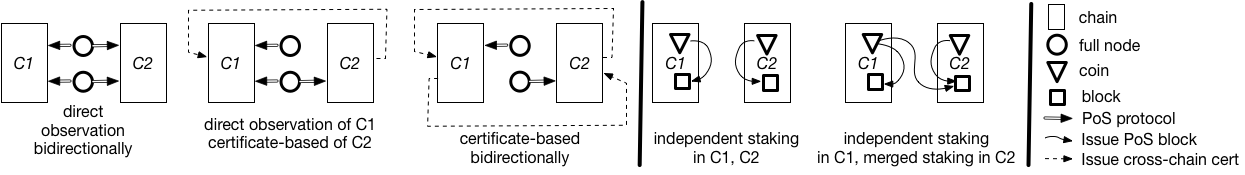
\includegraphics[width=\textwidth]{chapters/sidechains/figures/sidechains-options.png}
  \caption{Deployment options for PoS Sidechains.}
  \label{fig:sidechain-options}
  \end{center}
\end{figure*}

In our construction we choose an exemplary
configuration between two ledgers $\Ledger_1$ and
$\Ledger_2$, so that direct observation is applied to $\Ledger_1$,
cross-chain certification to $\Ledger_2$, independent-staking in $\Ledger_1$ and
merged staking in $\Ledger_2$.
As a result, all stakeholders in $\Ledger_2$ also keep track
of chain development on $\Ledger_1$ (and hence run a full node for $\Ledger_1$)
while the opposite is not necessary, i.e.,
$\Ledger_1$ stakeholders can be oblivious of transactions and
blocks being added to $\Ledger_2$.
This illustrates the two basic possibilities
of pegging and can be easily adapted
to  any other of the configurations between two ledgers in Figure~\ref{fig:sidechain-options}.

In order to reflect the asymmetry between the two chains in our exemplary
construction we will refer to $\Ledger_1$ as the ``mainchain'' $\Mainchain$, and to
$\Ledger_2$ as the ``sidechain'' $\Sidechain$. To elaborate further on this concrete
asymmetric use case, we also fully specify how the sidechain can be
initialized from scratch, assuming that the mainchain already exists.


%We also assume (as discussed in Section~\ref{sec:model}) that all
%actors have relatively synchronized clocks: i.e., clock drift is bounded
%and time can be divided in time slots that all parties can agree on.
%During the existence of the mainchain $\Mainchain$,
%the sidechain can come to existence whenever a new epoch starts on $\Mainchain$.

The pegging with the sidechain will be provided with respect to a specific asset of $\Mainchain$
that will be created on $\Mainchain$.
% PG: not used ever again
%and referred to as the \emph{home} asset of the
%whole sidechain ecosystem.
Note that $\Mainchain$ as well as $\Sidechain$ may carry
additional assets but for simplicity we will assume that staking and pegging is
accomplished only via this single primary asset.

The presentation of the construction is organized as follows. First, in Section~\ref{sec:ats} we introduce a novel
cryptographic primitive, \emph{ad-hoc threshold multisignature (ATMS)}, which is the fundamental building block for cross-chain certification.
Afterwards, in Section~\ref{sec:const} we use it as a black box to build secure
pegged ledgers with respect to concrete instantiations of the functions $\merge$
and $\effect$ and a validity language $\adalang$ for asset~$\ada$ given in Section~\ref{sec:inst}.
Finally, we discuss specific instantiations of ATMS in
Section~\ref{sec:auth}.


\import{chapters/sidechains/}{tms-definition.tex}
\import{chapters/sidechains/}{adalang.tex}

\subsection{The Sidechain Construction}
\label{sec:const}

We now describe the procedures for running a sidechain in the configuration
outlined at the beginning of this section: with independent staking on $\MC$ and
merged staking on $\SC$; direct observation of $\MC$ and
cross-chain certification of $\SC$.
We describe the sidechain's creation,
maintenance, and the way assets can be  transferred to it and back.  The
protocol we describe below is quite complex,
%(it entails 2 consensus protocols
%for maintaining both the mainchain and the sidechain, and a lot of connecting
%tissue)
%and to accommodate that, while still keeping the protocol description at
%a manageable length,
we hence choose to describe different parts of the protocol in
differing levels of detail. This level is always chosen with the intention to allow the
reader to easily fill in the details.
%, and to follow our security argument in Section~\ref{sec:security}.
A graphical depiction of our construction that can serve as a reference
%for the reader of the description below
is given in Figure~\ref{fig:sidechain}.
\begin{figure}[tb]%{{{
  \centering
  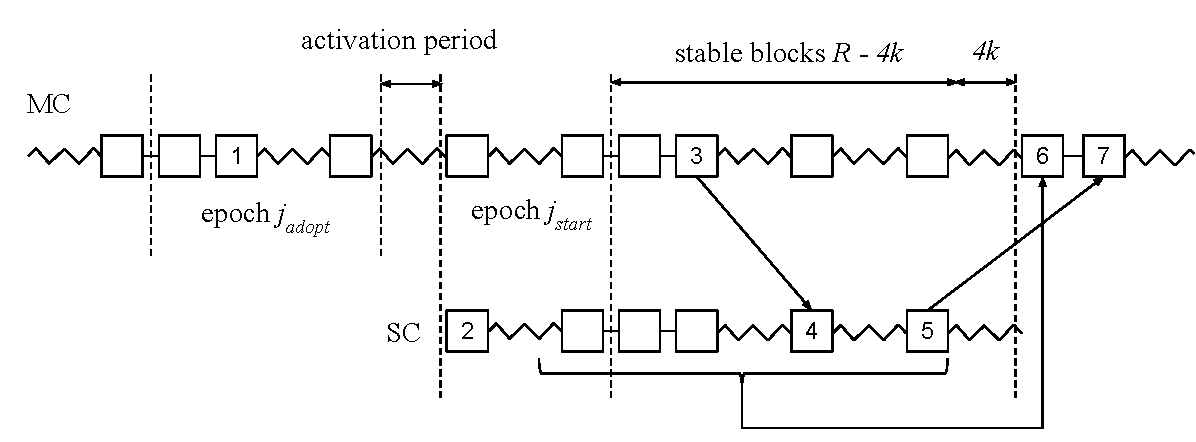
\includegraphics[width=0.8\textwidth]{chapters/sidechains/figures/sidechains-overview.pdf}
  \caption{
  Our sidechain construction. Blocks are shown as rectangles. Adjacent blocks
  connect with straight lines. Squiggly lines indicate some blocks are omitted.
  $\MC$ is at the top, $\SC$ at the bottom. Epochs are separated by dashed
  lines. $\epoch_{j_\text{adopt}}$ is the epoch of first signalling;
  $\epoch_{j_\text{start}}$ is the activation epoch. Blocks of interest: 1. The
  first block signalling $\SC$ awareness;
  2. The $\SC$ genesis block; 3. A $\tx_{\send}$
  transaction for a deposit; 4. A $\tx_{\rec}$ transaction for a
  deposit; 5. A $\tx_{\send}$ transaction for withdrawal; 6. A $\sccert$
  transaction signalling trust transition within $\SC$ and certifying pending
  withdrawals; 7. A $\tx_{\rec}$ transaction for withdrawal, certified in a $\sccert$
  transaction e.g. in block~6.
  }
  \label{fig:sidechain}
\end{figure}%}}}

\subsubsection{Notation}
Where applicable, we denote the analogues of the mainchain objects on the
sidechain with an additional overline.
%For instance, while $\SD_j$ denotes the
%stake distribution recorded on the mainchain by the latest block in
%the first $4k$ slots of epoch $j-1$ (which is the stake distribution used for
%sampling slot leaders for epoch $j$ on $\MC$), $\SDb_j$ will denote
%the stake distribution induced by the stake that resides on $\SC$ at the same
%slot (this would be the stake distribution used for sampling slot leaders for
%epoch $j$ if $\SC$ was using independent staking).
%Finally, we let  $\SDb^*_j$ denote  the distribution of stake
%that exists in either the sidechain or the mainchain, but has indicated
%sidechain adoption (as discussed below) by the end of the first $4k$ slots of epoch $\epoch_{j-1}$.
%This will be the stake
%distribution \emph{actually used} for leader election on $\SC$ in epoch $j$ as
%per the merged staking paradigm.
%
In our pseudocode, we use the statement
``\textbf{post} $\tx$ \textbf{to} $\Ledger$''
to refer to the
action of broadcasting the transaction $\tx$ to the maintainers of the ledger
$\Ledger$ so that they include it in the ledger eventually as prescribed by the
protocol.
Unless indicated otherwise, we also denote by $\stateMC$ (resp.
$\stateSC$) the current \emph{ledger state} of the ledger $\MC$ (resp. $\SC$) as
viewed by the party executing the protocol. Similarly, we denote by $\ChainMC$
(resp. $\ChainSC$) the currently held \emph{chain} corresponding to the ledger
$\MC$ (resp. $\SC$). Hence, for example $\stateMC$ always represents the state
stored in the stable part of the chain $\ChainMC$.

\subsubsection{Helper Transactions and Data}
The construction uses a set of \textit{helper transactions}
which can be included in both blockchains, but do not get reported
in the respective ledgers. These helper transactions store the appropriate
metadata which is implementation-specific and allow the pegging functionality to be
maintained. The transaction types $\mathsf{side}\-\mathsf{chain\_support}$,
$\mathsf{side}\-\mathsf{chain\_certificate}$,
$\mathsf{side}\-\mathsf{chain\_success}$ and
$\mathsf{side}\-\mathsf{chain\_fai}\-\mathsf{lure}$, whose nature will be
detailed later, are of this kind.
Moreover, our concrete implementation of pegged ledgers extends certain
transactions with additional information (such as Merkle-tree inclusion proofs)
that are, for convenience, understood to be stripped off these transactions when
the blockchain is interpreted as a ledger.

\subsubsection{Initialisation}

The creation of a new sidechain~$\SC$ starts by any of the stakeholders of the
mainchain adopting the code that implements the sidechain. This action does not
require the stakeholders to put stake on the sidechain but merely to run the
code to support it (e.g. by installing a pluggable module into their client
software). In the following this is referred to as ``adopting the sidechain''
and captured by the predicate $\SidechainAdoption$.
The adoption is  announced at the mainchain by a special transaction
detailed below.  Each sidechain is identified by a unique identifier $\id_\SC$.
%The identifier is a simple string,
%which must be chosen to be unique for that particular sidechain,
%. For example,
%the first attempt at launching a smart-contract-supporting sidechain could have
%the identifier
%e.g. ``\texttt{computation\_layer\_1.0.0}''. As mentioned, we consider a
%single sidechain which we will refer to as $\SC$, but our results extend to
%multiple sidechains sharing the same mainchain.

Let $\jadopt$ denote the epoch on $\MC$ when the first adoption transaction has
appeared; the sidechain $\SC$ -- if its activation succeeds as discussed
below -- will start at the beginning of some later epoch $\jstart$ and will have
its slots and epochs synchronized with $\MC$.
The software module implementing the sidechain comes with a set of
deterministic rules describing the requirements for the successful activation of
the sidechain, as well as for determining $\jstart$.
These rules are sidechain-specific and are captured in a predicate
$\ActSuccess$ and a function $\ActEpoch$, respectively.
One typical such example is the following:
the sidechain starts at the beginning of $\MC$-epoch $\jstart$ for the smallest
$\jstart$ that satisfies:
%\begin{itemize}
  %\item
    (i)  $\jstart - \jadopt > c_1$;
  %\item
    (ii) at least $c_2$-fraction of stake on $\MC$ is controlled by stakeholders that
    have adopted $\SC$;
%\end{itemize}
for some constants $c_1$,$c_2$. Additionally, if such a successful activation
does not occur until a failure condition captured by a predicate
$\ActFail$ is met (e.g. until a predetermined period of $c_3>c_1$ epochs has
passed), the sidechain initialization is aborted.
%The exact mechanics of the abortion procedure are also left to be
%determined by the sidechain module (we denote them as $\SC.\Cleanup()$)
%but they include straightforward actions such
%as removing the module that supports the sidechain and erasing any other data
%structure associated with it.
%\footnote{We note that there is nothing that
%prevents a minority of $\MC$ stakeholders from continuing to support an aborted
%sidechain if they insist, in violation of the sidechain creation rules. However
%all the other stakeholders of $\MC$ will consider the sidechain as failed, and
%assuming they represent the majority of stake, any blocks produced by the
%diverging stakeholders that reference the failed sidechain will be collectively
%removed from the ledger of $\MC$. On the other hand, if the majority of stake in
%$\MC$ insists on the violation of the sidechain creation rules, we observe that
%the constants $c_1,c_2$ can be effectively changed by a soft-fork of $\MC$. Such
%soft-forks can be avoided by choosing relatively low values for $c_1,c_2$. On
%the other hand, it is important to note that really low values for $c_1,c_2$ may
%result in unnecessarily cluttering the $\MC$ with data related to sidechains
%that are spuriously created. }

%%Suppose the first occurrence of sidechain adoption is
%%announced by a stakeholder at epoch $j^*$ of $\MC$ for some $j^* \geq 2$. Then the
%%sidechain will be created at epoch $\epoch_j$ for some $j > j^*$. The sidechain
%%genesis block is created at the first slot of epoch $\epoch_j$.

%The way $j$ is determined based on $j^*$ is as follows. Each sidechain defines
%an \textit{activation predicate} $\on^{\ell_1, \ell_2, \ell_3}(\Chain[:-k])$,
%parameterized by integers $\ell_1, \ell_2, \ell_3 \in \N$, which is evaluated on
%the stable part $\Chain[:-k]$ of some chain $\Chain$. At every slot after epoch
%$j^*$, the honest stakeholders on the network evaluate the predicate $\on$ on the
%growing stable part of the mainchain $\Chain[:-k]$, where $\Chain$ is their
%currently locally adopted mainchain.

%The predicate $\on^{\ell_1, \ell_2, \ell_3}(\Chain)$ checks that all of the following conditions are
%satisfied:
%\begin{enumerate}
%    \item The chain length is sufficient: $|\Chain| > \ell_1$.
%    \item Sufficient stake has been moved into limbo: $|\SDb| > \ell_2$
%          (the exact definition of stake movement will follow momentarily).
%    \item Sufficient stake is aware of the sidechain: $|\SDb^*| > \ell_3$
%          (the exact definition of stake awareness will follow momentarily).
%    \item There is a sufficient epoch gap:
%          If the first adoption announcement occurred after or at slot
%          %$R - 2k/f$
%          $R - 2k$
%          of epoch $\epoch_{j^*}$, the current slot must belong to $\epoch_j$, with
%          $j > j^*$.
%\end{enumerate}
%The sidechain is considered activated during the first slot at which its
%$\on^{\ell_1, \ell_2, \ell_3}$
%predicate is evaluated to \textit{true}. The genesis block $\Genesisb$ of the
%sidechain is then created at the first slot of the first epoch after the slot
%during which the sidechain was activated.

%Each sidechain also defines an \textit{expiration predicate}
%$\off^{\ell_4}(\Chain[:-k])$, parameterized by $\ell_4 \in \N$, which is also
%evaluated on the stable part of the mainchain. As long as the sidechain has not
%yet been activated, at every slot after epoch $j^*$, each honest maintainer
%evaluates the predicate $\off$ on the growing stable part of the mainchain
%$\Chain[:-k]$, where $\Chain$ is their currently locally adopted mainchain. The
%predicate $\off$ checks whether the chain length is too large: $|\Chain| >
%\ell_4$.
%If at some slot the predicate $\off(\Chain)$ evaluates to \textit{true} while at
%the same slot the predicate $\on(\Chain)$ evaluates to \textit{false}, then the
%sidechain creation is abandoned and we say that the sidechain creation has
%\textit{expired}. No sidechain genesis block $\Genesisb$ is created. Of course,
%for meaningful sidechains, we have that $\ell_4 > \ell_1$ to give the sidechain
%a period of time during which it can be created. If a sidechain's creation
%expires, then it will never be created. An attempt can be made in the future to
%create a new sidechain with the same features, but with a new identifier.

%During the period after the first awareness announcement block and before the
%sidechain is created or expires, we allow stake to be moved from the mainchain
%to the sidechain. The mechanics for the stake transfers is described later in
%this section. For now, suppose there is a way to move money out of the mainchain
%via a $\mathsf{sidechain\_send}$ transaction which is included in a mainchain
%block. As the sidechain has not yet been created, this money is kept in
%\textit{limbo} in that it has been moved out of the mainchain but not yet into
%the sidechain, in the sense that it cannot yet be recovered. If the sidechain is
%successfully created at epoch $\epoch_j$, then the money in limbo that was moved
%from the mainchain into the sidechain during the period after the first
%awareness announcement and until the first activation can be recovered into the
%sidechain. This recovery can happen during the sidechain genesis block or at
%later blocks. However, if the sidechain creation expires, then the money in
%limbo can be returned to its previous owners on the mainchain by issuing dual
%reverting transaction, $\mathsf{sidechain\_recover}$, and including it on the
%mainchain.

The activation process then follows the steps outlined below, the detailed
description is  given in
%Appendix~\ref{sec:algorithms} as
Algorithm~\ref{alg.init}).
\import{chapters/sidechains/}{algorithms/alg.sc-init}
%\begin{enumerate}
%\item
    First, every stakeholder $U_i$ of $\MC$ (holding a key pair $(vk,sk)$) that supports the sidechain
    posts a special transaction
    $
    \mathsf{sidechain\_support}(\id_\SC,vk,vk')
    $,
    signed by $sk$
    into the mainchain. Here $vk'$ is a public key from an ATMS key pair
    freshly generated by $U_i$; its role is explained in Section~\ref{sec:trust}
    below.
    %at blocks created after epoch $j^*$.
    %, where
    %the initial adoption stakeholder distribution $\SDb^*_{j^*}$ of the
    %sidechain is initially empty.

  %\item
    If the sidechain activation succeeds, then during the first slot of epoch $\jstart$
    the stakeholders of $\MC$ that support $\SC$  construct the genesis block
    $
    \Genesisb
    =(
      \id_\SC,
      \SDb_{\jstart},
      \rndb_{\jstart}\defeq H( \id_\SC, \rnd_{\jstart}),
      \params,
      avk^{\jstart}
    )
    $
    for $\SC$. $\rnd_{\jstart}$ is the
    randomness for leader election on $\MC$ in epoch $\jstart$ (derived
    on $\MC$ in epoch $\jstart-1$). It is reused to compute the
    initial sidechain randomness
    $\rndb_{\jstart}$ as well, further
    $\rndb_{j'}$ for $j'>\jstart$ are determined independently on $\SC$ using
    the Ouroboros coin-tossing protocol.\footnote{This can be interpreted as
    using $\MC$ to implement the setup functionality needed to bootstrap $\SC$.
    }
    Furthermore, $\params$ and $avk^{\jstart}$ are public parameters and an aggregated public
    key of an ATMS scheme; their creation and role is
    discussed in Section~\ref{sec:trust} below.
    Note that $\Genesisb$ is defined mostly for notational compatibility, as
    $\SDb_{\jstart}$ is empty at this point anyway.
    %Note that this requires
    %$j\geq j^*+2$, as $\SDb_{j'}$ for $j'<j+2$ are empty. This can be enforced
    %as a part of the $\on$ predicate.
    $\Genesisb$ can be constructed as soon as %both $\SDb_{\jstart}$ and
    $\rnd_{\jstart}$ is known and stable.
    %, which is true as soon as the mainchain is stable up to
    %slot $16k/f$ of epoch ${j-1}$.

  %\item
    The stakeholders that adopted $\SC$ post into $\MC$
    %in the first block of epoch $\epoch_j$
    a transaction $\mathsf{sidechain\_success}(\id_\SC)$ to
    signify that $\SC$ has been initialized.
    If the sidechain creation expires, then, after the first block of the next
    epoch after expiration occurs, the stakeholders of $\MC$ that supported
    $\SC$ post the transaction $\mathsf{sidechain\_failure}(\id_\SC)$ to $\MC$.
    We assume that both predicates $\ActSuccess$ and $\ActFail$ can be evaluated
    based on the state of $\MC$ only, and hence spurious success/failure
    transactions will be considered invalid.
    %Upon
    %posting this message, refund transactions can be issued on the mainchain.

%\end{enumerate}

%Note that as soon as a sidechain is created it holds that an initial
%stakeholder distribution for the sidechain is known by the maintainers of the
%ledger state of $\MC$. We will maintain this property: the $\MC$ ledger state
%will always have a relatively current commitment to the stakeholder distribution
%of $\SC$.

%\newpage

\subsubsection{Maintenance}

Once the sidechain is created, both the mainchain and the sidechain need to be
maintained by their respective set of stakeholders (detailed below) running
their respective instance of the Ouroboros protocol.
%. In both
%cases this is done by running a slightly modified version of the Ouroboros
%protocol as follows.

In the case of the mainchain, the maintenance procedure is given
in Algorithm~\ref{alg.maintain.MC}.
This algorithm is run by all stakeholders controlling stake that is recorded on
the mainchain. Each stakeholder, on every new slot, collects all the candidate
$\MC$-chains from the network (modelled via the $\Diffuse$ functionality) and
filters them for both consensus-level validity (using $\MC.\ValidConsLevel$) and
transaction validity (using the $\verifierMC$ predicate given in
Algorithm~\ref{alg.mainchain}). Out of the remaining valid chains, he chooses
his new state $\Chain_{\MC}$ via $\PickWinningChain$. Then the stakeholder
evaluates whether he is an eligible leader for this slot, basing its selection
on the stake distribution $\SD_j$ and randomness $\rnd_j$, which are determined
once per epoch
%in the $\SwitchMCEpoch$ function
in accordance with the Ouroboros protocol.
If the stakeholder finds out he is a slot leader, he creates a new block $B$ by
including all transactions currently valid with respect to $\Chain_{\MC}$
(as per the predicate $\verifierMCtx$ given also in Algorithm~\ref{alg.mainchain}),
appends it to the chain $\Chain_{\MC}$ and diffuses the result\footnote{
As in~\cite{C:KRDO17,EC:DGKR18}, we simplify our
presentation by diffusing the complete chains,
although a practical implementation would only diffuse the block $B$.}
for other parties to adopt.

\import{chapters/sidechains/}{algorithms/alg.mc-maintain.tex}
\import{chapters/sidechains/}{algorithms/alg.mainchain.tex}

The maintenance procedure for $\SC$ is similar, hence we only
describe here how it differs from Algorithm~\ref{alg.maintain.MC}. Most
importantly, it is executed by all stakeholders who have adopted $\SC$,
irrespectively of whether they own any stake on $\SC$.
Recall that the slots and epochs of the $\SC$-instance of Ouroboros are aligned
with the slots and epochs of $\MC$.

The first difference is that all ocurrences of $\MC$ and $\ChainMC$ are
naturally replaced by $\SC$ and $\ChainSC$, respectively.  This also means that
the validity of received chains (resp. transactions), determined on
line~\ref{line:filter} (resp.~\ref{line:filtertx}), is decided based on
predicate
$\verifierSC(\cdot,\ChainMC)$ (resp.
$\verifierSCtx(\cdot)$)
instead of
the predicate
$\verifierMC(\cdot)$ (resp.
$\verifierMCtx(\cdot)$). Additionally, note that $\verifierSCtx$ must be called
with a sequence of transactions containing both the transactions in $\SC$ as
well as the transactions in $\MC$ interspersed and timestamped, similarly to the
way done in Line~\ref{alg.sidechain.interspersing} of
Algorithm~\ref{alg.sidechain}. This is straightforward to implement, as the
sidechain maintainers also directly observe the mainchain. The predicates
$\verifierSCtx$
and
$\verifierSC$
are given in
Algorithms~\ref{alg.sidechain-tx}
and~\ref{alg.sidechain}, respectively.

\import{chapters/sidechains/}{algorithms/alg.sidechain-figure.tex}

Second, instead of the
%the procedure $\SwitchMCEpoch$ on
%line~\ref{line:switch} is replaced by the procedure $\SwitchSCEpoch$ (given in
%Algorithm~\ref{alg.maintain.SC}) that determines a different
stake distribution $\SD_j$ determined on line~\ref{line:SD}, a different
distribution $\SDb^*_j$ is determined to be used for slot leader selection in
the $j$-th epoch of the sidechain.  The distribution $\SDb^*$ contains all
stake belonging to stakeholders that have adopted $\SC$, irrespectively of
whether this stake is located on $\MC$ or $\SC$ (we call such stake
\emph{$\SC$-aware}).  It can be obtained by combining the distribution $\SDb$ as
recorded in $\SC$ with the distribution of $\SC$-aware stake on $\MC$ (which is
known to $\SC$-maintainers via direct observation of $\MC$).
%This is
%in contrast to a hypothetical stand-alone execution of Ouroboros  on $\SC$,
%which would only use the stake distribution $\SDb$ instead.
Note that the
distribution used for epoch $j$ reflects the stake distribution of $\SC$-aware
stake in the past, namely by slot $4k$ of epoch $j-1$, just as in $\MC$.
%The randomness $\rndb_{j}$ for each epoch $j$
%is derived deterministically from the mainchain randomness for the same
%epoch $\rnd_j$, concretely $\rndb_{j}\defeq H(\id_\SC, \rnd_{j})$.
%This is done for efficiency reasons as the randomness in Ouroboros is
%derived via a relatively costly coin-tossing protocol, and its reuse on the
%sidechain does not harm security.
Naturally, this also implies that the fourth parameter for the $\SlotLeader$ predicate on
line~\ref{line:leader} is  $\SDb^*_j$ %and $\rndb_j$
instead of $\SD_j$.
% and $\rnd_j$, respectively.

Finally, the block construction procedure on line~\ref{line:construct} is
adjusted so that in the last $2k$ slots of each epoch, the created blocks on the
sidechain also
contain an additional ATMS signature of a so-called sidechain certificate (how
this certificate is constructed and used will be described below). Hence,
whenever $\slot\mod R>10k$, line~\ref{line:construct} is replaced by
$
  B
  \leftarrow
  (\prev,\vec\tx_{\valid},\sigma,\sigma_{\sccert_{j+1}})
$
where
$\sigma_{\sccert_{j+1}}=\Sig_{sk}(\sccert_{j+1})$ and $j$ is the current epoch index.

%\import{chapters/sidechains/}{algorithms/alg.sc-maintain.tex}

%\newpage

\subsubsection{Depositing to $\SC$}

Once $\SC$ is initialized, cross-chain transfers to it can be made from $\MC$.
A cross-chain transfer operation in this
case consists of two transactions $\tx_{\send}$ and $\tx_{\rec}$ that both have
$\send=\MC$, $\rec=\SC$, and all other fields are also identical, except that
each $\tx_i$ for $i\in\{\send,\rec\}$ contains $\llid=i$.
%(and of course, the signatures differ as well).
The \emph{sending transaction} $\tx_{\send}$ is
meant to be included in $\MC$, while the \emph{receiving transaction} $\tx_{\rec}$ is meant to be included in
$\SC$.

%\begin{enumerate}[resume]
  %\item
    Whenever a stakeholder on $\MC$ that has adopted $\SC$  wants to transfer funds to $\SC$, she
    diffuses $\tx_{\send}$ with the correct receiving account on
    $\SC$ and the desired amount.
    %, which contains as an
    %additional information an address $\recAccount$ in $\SC$ where the funds
    %should arrive. If the transaction is issued %in limbo
    %before $\SC$ is activated,
    %then it also includes
    %an address $\recAccount'$ in $\MC$ where the funds can be recovered in case
    %the creation of the sidechain is abandoned.
    Honest slot leaders in $\MC$
    include these transactions into their blocks just like any
    intra-chain transfer transactions.
    %In the validity language $\tilde\ValLang_\Asset$,
    %the $\mathsf{sidechain\_send}$ transactions appear
    %as transactions with $\send \neq \rec$ and $\llid = \send$.
  %\item
    Maintainers of $\MC$ keep account of a variable $\pool_{\SC}$, initially set
    to zero. Whenever a $\tx_{\send}$ is included into $\MC$, they increase
    $\pool_{\SC}$ by the amount of this transaction.

  %\item
    When $\tx_{\send}$ becomes stable in $\MC$ (i.e., appears in
    $\stateMC$, this happens at
    most $2k$ slots after its inclusion),
    the stakeholder creates and diffuses the corresponding $\tx_{\rec}$
    which credits the respective amount of coins to $\recAccount$ in $\SC$,
    to be included into $\SC$.
    %a $\mathsf{sidechain\_receive}$ transaction on
    %$\SC$ to receive the funds into $\recAccount$ on $\SC$.
    %For any
    %$\mathsf{sidechain\_send}$ transaction $\tx$ we have
    %$\eff{\MC}{\SC}(\tx) = \tx$ where $\tx'$ is the
    %$\mathsf{sidechain\_receive}$ transaction corresponding to $\tx$,
    %and honest slot leaders in $\SC$ include these transactions into their
    %blocks (to satisfy pegging correctness).
    %The transaction $\tx_{\rec}$ credits the respective amount
    %of coins to $\recAccount$ in $\SC$.
    In practice, this is akin to a coinbase
    transaction, as the money was not transferred from an existing $\SC$
    account.
    %with sufficient funds.
    %The inclusion of $\mathsf{sidechain\_receive}$ into
    %the $\SC$ can only happen as soon as the sidechain has been created; otherwise,
    %the money remains \textit{in limbo} until either the sidechain is created or
    %its creation expires. In the validity language $\tilde\ValLang_\Asset$, the
    %$\mathsf{sidechain\_receive}$ transactions appear as transactions with
    %$\send \neq \rec$ and $\llid = \rec$.

  %\item
  %  If the sidechain creation expires, the stakeholder diffuses a
  %  $\mathsf{sidechain\_recover}$ to $\MC$ which returns the funds from
  %  limbo to the recovery address $\recAccount'$ in $\MC$. For conciseness, we
  %  do not detail the structure of $\mathsf{sidechain\_recover}$ transactions
  %  in the validity language, as it is immaterial to the correctness and
  %  security of the scheme. The $\mathsf{sidechain\_recover}$ transactions can be
  %  considered as $\mathsf{sidechain\_receive}$ transactions which recover funds
  %  into $\recAccount'$ of $\MC$.

%\end{enumerate}

Note that depositing from $\MC$ to $\SC$ is relatively fast; it merely requires
a reliable inclusion of $\tx_{\send}$ into $\MC$ and
consequently of $\txrec$ into $\SC$, as guaranteed
by the liveness of the underlying Ouroboros instances.
%the coins can be moved from $\MC$ to $\SC$ in at most $8k/f$ slots ($4k/f$ to
%reliably include $\mathsf{sidechain\_send}$ into $\MC$, and $4k/f$ to reliably
%include  $\mathsf{sidechain\_receive}$ into $\SC$).
The depositing algorithm code is shown in
%Appendix~\ref{sec:algorithms} as
Algorithm~\ref{alg.deposit}.
\import{chapters/sidechains/}{algorithms/alg.depositing}


\subsubsection{Withdrawing to $\MC$}

The withdrawal operation is more cumbersome than the depositing
operation since not all nodes of $\MC$ have adopted (i.e., are aware of and follow) the
sidechain $\SC$.
As transactions, the withdrawals have the same structure as deposits, consisting
of $\tx_{\send}$ and $\tx_{\rec}$, with the only difference
that now they both have $\send=\SC$ and $\rec=\MC$.
The sending transaction will be handled in the same way as in the case of
deposits, but the receiving transaction requires a different certificate-based
treatment, as detailed below.

%\begin{enumerate}[resume]
  %\item
    Whenever a stakeholder in $\SC$ wishes to withdraw coins from $\SC$
    to $\MC$, she creates and diffuses the respective transaction $\tx_{\send}$
    with the correct transfer details as before.
    If $\tx_{\send}$ is included in a block that belongs in one of the first
    $R-4k$ slots of some epoch then let $\jsend$ denote the index of this epoch,
    otherwise let $\jsend$ denote the index of the following epoch.
  %\item
    The stakeholder then waits for the end of the epoch $\epoch_{\jsend}$ to pass and
    $\epoch_{\jsend+1}$ to begin.

  %\item
    At the beginning of $\epoch_{\jsend+1}$, a special transaction called
    \emph{sidechain certificate
    $\sccert_{\jsend+1}$} is generated by the maintainers of $\SC$.
    It contains:
    %\begin{itemize}
      %\item
        (i) a Merkle-tree commitment to all withdrawal transactions $\tx_{\send}$ that were
        %the total inflow of funds from $\MC$ to $\SC$,
        %summarizing all $\mathsf{sidechain\_send}$ transactions that were
        included into $\SC$ during last
        %$4k/f$
        $4k$ slots of epoch $\jsend-1$ and
        the first
        %$20k/f$
        $R-4k$ slots of epoch $\jsend$ (as these all are already stable by slot
        $R-2k$ of epoch $\jsend$);
      %\item
        (ii) other information allowing the maintainers of $\MC$ to
        inductively validate the certificate in every epoch.
        %the stake distribution $\SDb_{j'+1}$ (which is known to the
        %stakeholders following both $\SC$ and $\MC$, can be used to derive
        %$\SDb^*_{j'+1}$ by anyone following $\MC$); and
    %\end{itemize}
    %that that certain transactions moving
    %money from $\SC$ to $\MC$ are pending.
    %and a certain amount of
    %funds is waiting for withdrawalunts.
    The construction of $\sccert$ is detailed  below, for now  assume
    that the transaction provides a proof that the included information about
    withdrawal transactions is correct.
    %shifting and pending transactions have taken place in $\SC$.
    %Concrete constructions will be provided in the next section.
  %\item
    The transaction $\sccert$ is broadcast into the
    $\MC$ network to be
    included into $\MC$ at the beginning of $\epoch_{\jsend+1}$ by the first honest
    slot leader.

  %\item
    The stakeholder who wishes to withdraw their money into $\MC$ now creates
    and diffuses the transaction $\tx_{\rec}$ to be included in~$\MC$.
    %which includes a reference to the
    %respective $\sccert$ transaction, along with a
    %proof that they are the rightful owner which should receive the incoming
    %funds.
    This transaction is only included into $\MC$ if it is considered valid,
    which means:
    (1) it is properly signed;
    (2) it contains a Merkle inclusion proof confirming its presence in some
    already included sidechain certificate;
    (3) its amount is less or equal to the current value of $\pool_{\SC}$.
    If included, $\MC$-maintainers decrease the value of $\pool_{\SC}$ by the
    amount of this transaction.
%\end{enumerate}
The code of the withdrawal algorithm is illustrated in
Algorithm~\ref{alg.withdraw}.

\import{chapters/sidechains/}{algorithms/alg.withdraw}

%\newpage
\subsubsection{The certificate transaction}
\label{sec:sccert}

We now describe the construction of the $\sccert$ transaction, also called the
\emph{sidechain certificate}, formally described in
Algorithm~\ref{alg.sccert}).
\import{chapters/sidechains/}{algorithms/alg.cert}
The role of the
certificate produced by the end of epoch $j-1$ to be included in $\MC$ at
the beginning of epoch ${j}$ (denoted $\sccert_{j}$)  is to attest
all the withdrawals that had their sending transactions included
into $\SC$
%to $\MC$ by including a $\tx_{send}$ transaction into
%$\SC$
in either the last $4k$ slots of $\epoch_{j-2}$ or the first $R-4k$ slots
of $\epoch_{j-1}$.
To maintain a chain of trust for the $\MC$ maintainers that cannot
verify these transactions by observing $\SC$, we make use of
ad-hoc threshold multisignatures introduced in Section~\ref{sec:ats}.
Namely, the $\sccert_{j}$ transaction
also contains an aggregate key $avk^{j}$ of an ATMS, and is signed by the
previous aggregate key $avk^{j-1}$ included in $\sccert_{j-1}$.

$\sccert_{j}$ is generated by $\SC$-maintainers
%examining the
%sequence of all transactions $\vec\tx$ which are included in $\SC$ during those
%$R$ slots
and contains:
\begin{itemize}
    \item
          \textbf{The epoch index $j$}.
    \item
          \textbf{The pending transactions from $\SC$ to $\MC$.}
          Let $\vec\tx$ be the sequence of all transactions
          which are included in $\SC$ during either
          the last $4k$ slots of $\epoch_{j-2}$ or the first $R-4k$ slots of
          $\epoch_j$. All transactions in $\vec\tx$ that have $\SC=\send \neq \rec=\MC$
          are picked up and combined into a list $\pending_{j}$ (sorted in the
          same order as in $\SC$). Let $\commit{\pending_{j}}$ denote a Merkle-tree commitment to
          this list.

    \item
          \textbf{The new ATMS key $avk^{j}$.}
          The key is created from the public keys of the slot
          leaders of the last $2k$ slots of the epoch $j$, using
          threshold $k+1$. Hence, it allows to verify whether a particular signature comes
          from $k+1$ out of these $2k$ keys.
    \item
          \textbf{Signature valid with respect to $avk^{j-1}$.}
\end{itemize}
The full $\sccert_{j}$ is therefore a tuple
$\left(j,\langle\pending_{j}\rangle,avk^{j},\sigma_{j}\right)$,
where $\sigma_{j}$ is an ATMS signature on the preceding elements that verifies
using $avk^{j-1}$.

The certificate $\sccert_{j+1}$ is constructed as follows:
Both the stake distribution
$\SDb^*_{j+1}$ and the $\SC$-randomness $\rndb_{j+1}$ (and hence also the slot leader
schedule for $\SC$ in epoch $j+1$)
are determined by the states of
the blockchains $\MC$ and $\SC$ by the end of slot $10k$ of epoch $j$.
Therefore, during the last $2k$ slots of epoch $j$, the $2k$ elected slot
leaders for these slots can already include a (local) signature on (their
proposal of) $\sccert_{j+1}$ into the blocks they create. Given the
deterministic construction of $\sccert_{j+1}$, all valid blocks ending up in
the part of $\SC$-chain belonging to the last $2k$ slots of epoch $j$ will
contain a local signature on the same $\sccert_{j+1}$,
and by the chain growth
property of the underlying blockchain, there will be at least $k+1$ of them.
Therefore, any party
observing $\SC$ can now combine these signatures into an ATMS that can be later
verified using the ATMS key $avk^j$, it can hence create the complete certificate
$\sccert_{j+1}$ and serve it to the maintainers of $\MC$ for inclusion.

%This includes two pieces of data into $\sccert$: The hash of the transactions
%Merkle tree root and the new aggregate key $avk^{j+1}$.
%Both of these are referenced in future blocks:

%\begin{enumerate}
%    \item \textbf{Inclusion in the pending transactions.}
%        Every $\tx_{\rec}$ transaction needs to prove,
%        through a Merkle-Patricia trie proof-of-inclusion, that they are the
%        rightful owner of a spending transaction $\tx_{\rec}$.
%        This proof-of-inclusion proves that the claimed account and amount are
%        in the tree root certified by $\sccert$. The
%        validator needs to also check that there is no double spending
%        by keeping track of which $\sccert$ references
%        are already spent and avoiding replays.

%    \item \textbf{The aggregate key $avk^{j}$.}
%        This key is used to sign-off the transition to the next key $avk^{j+1}$.
%\end{enumerate}

%\subsubsection{Advancing to next epoch.}
%\TODO{probably not needed}

%Each $j^\text{th}$ $\SC$ epoch maintains an \emph{epoch key} $avk^{j}$ which
%corresponds to a uniform sample, by stake, of the protocol participants. These
%$avk^{j}$ keys are committed to the mainchain and are used to sign off the
%transition to a new epoch key $avk^{j+1}$ at the end of each epoch. They are
%also used to sign off the collection of transactions in the form of
%$\tx_{\send}$ committed to the sidechain, which are leaving the sidechain and
%are entering the mainchain.

%The epoch key works as follows: During each epoch, the last $2k$ slot leaders of
%that epoch are elected by the underlying Ouroboros consensus mechanism as usual.
%The honest majority security assumption mandates that at least $k+1$ are honest.
%These $2k$ local keys $\{vk_i\}$ are then combined using an aggregate
%$(k+1)$-threshold signature scheme $\KeyCombine$ to produce an aggregate key
%$avk$. Whenever the sidechain maintainers wish to produce a statement $m$ about
%the sidechain which the majority authorizes, they can do so using $k+1$ of
%these $2k$ keys. Because at least $k+1$ of these keys are honest, at least $k+1$
%local signatures $s_i$ will be produced. Any sidechain maintainer can then
%combine them into an aggregate signature $\sigma \gets \SigCombine(\{s_i\})$.
%The aggregate signature can then be verified by anyone who knows that $avk$ is
%authentic by evaluating $\VerCombined(avk, \sigma, m)$.

%In order for the sidechain $\SC$ to advance from epoch $\epoch_j$ to
%$\epoch_{j+1}$ the $\MC$ stakeholders will need to update the $avk$ that they
%hold about the sidechain.

%Both of these pieces of data, i.e., the transition to the new $avk$ as well as
%the commitment to the sidechain $\tx_{\send}$ transactions are collected into
%an $\sccert$ transaction which is produced by the sidechain maintainers and
%diffused on the mainchain network for inclusion into the mainchain. Details
%follow.

%\noindent\textbf{Transitioning trust.}
\subsubsection{Transitioning trust}
\label{sec:trust}

As already outlined above, our construction uses ATMS
to maintain the authenticity of the sidechain certificates from epoch to epoch.
We now describe this inductive process in greater detail.

%We have still intentionally left open how the authenticity of the
%$\sccert$ transaction is proven. Without such a proof, a
%malicious party could claim an incorrect key $avk$ or pending
%transactions. To do this, we incorporate our \emph{aggregate threshold signature
%scheme} primitive as defined earlier. Specifically, the scheme works by relaying
%trust from epoch to epoch inductively.

Initially, during the setup of the sidechain, $\params \gets
\GenParam(1^\kappa)$ is ran. Stakeholders generate
%all players who will ever hold stake generate
their keys by invoking $(sk_i, vk_i) \gets \Gen(\params)$.
In case $\Gen(\cdot)$ is a probabilistic algorithm, it is run in a derandomized
fashion with its coins fixed to the output of a PRNG that is seeded by
$H(\mathsf{ats\_init}, \rnd_{\jstart})$ where ``$\mathsf{ats\_init}$'' is a fixed
label and $H$ is a hash function. This ensures that $\params$ will
be uniquely determined and will still be unpredictable. We note
that this process is only suitable for ATMS that employ public-coin parameters;
our ATMS constructions in Section~\ref{sec:auth} are only of this type.

For the induction base, $\params$ is published as part of the Genesis block
$\Genesisb$.
%The Genesis block is accompanied also by an initial stake
%distribution $\SDb_0$ to be used during the very first epoch of the sidechain
%$\epoch_0$. During epoch $\epoch_0$ the last $2k$ slot leaders are elected by
%the Ouroboros protocol and so are known to all sidechain maintainers. The
%collection of these $2k$ keys constitutes the first \emph{trust committee} of
%the sidechain. Since there exists no previous committee to attest to its
%legitimacy, each of these $2k$ keys are included in the mainchain as part of
%its initialization (together with the sidechain identifier).
%\aggelos{There should be a better way to do this without directly burdening
%the $\MC$ with more information. For example,
Each time an $\MC$ stakeholder $U_i$
posts the
$\mathsf{sidechain\_support}$ message to $\MC$, he  also includes an ATMS key $vk_i$.
Subsequently,
when the $\SC$ is initialised, the
stake distribution $\SDb^*_{\jstart}$ is known to the $\MC$ participants. Hence,
based on $\SDb^*_{\jstart}$ and $\rndb_{\jstart}$,
these can determine the last $2k$ slot leaders of epoch $\jstart$ in $\SC$,
we will refer to them as the $\jstart$-{th} \emph{trust committee}.
(In general, the $j$-th \emph{trust committee} for $j\geq\jstart$ will be the set
of last $2k$ slot leaders in epoch $j$.)
%$\MC$-maintainers (and thus also $\SC$-maintainers) can
$\SC$-maintainers (that also follow $\MC$) can also determine the $\jstart$-{th} trust committee
and therefore create $avk^{\jstart}$ from their public keys and insert it into
the genesis block $\Genesisb$ of  $\SC$. They can also serve it as a special
transaction to the $\MC$-maintainers to include into the mainchain.
The correctness of $avk^{\jstart}$ can be
readily verified by anyone following the mainchain using the procedure
$\Comprises$ of the used ATMS.

%\TODO{
%These keys are
%then combined into the first epoch's committee key $avk^0 \gets
%\KeyCombine(\{vk^0_i: i \in [2k]\})$, where $\{vk^0_i: i \in [2k]\}$ is the set
%of public keys corresponding to the last $2k$ slot leaders of the epoch. Anyone
%can generate this key and checking its validity requires verifying
%that $\Comprises(\mathcal{VK}^0, avk^0)$ is \emph{true}. An honest $\MC$ slot
%leader extending a blockchain not containing a commitment to a valid $avk^0$
%will include $avk^0$ into their block. Any $\MC$ maintainer can verify if this
%$avk^0$ is valid and reject blocks that include invalid values.  This allows the
%mainchain maintainers to reach consensus about the first trust committee key
%after the first claimed key $avk^0$ has been buried under $k$ blocks.
%}

For the induction step, consider an  epoch $j>\jstart$ and assume that
there exists an ATMS key of the previous epoch $avk^{j-1}$,
known to the mainchain maintainers.
%These keys are then
%collected into a combined key $avk^j \gets \KeyCombine(\{vk^j_i:
%i \in [2k]\})$ by any $\SC$ maintainer.
Every honest $\SC$ slot leader
among the last $2k$ slot leaders of $\SC$ epoch $j-1$ will produce a local
signature $s^j_i$ on the message $m = (j,\langle\pending_j\rangle,avk_j)$
using their private key $sk^{j-1}_i$ by running $\Sig(sk^{j-1}_i, m)$, and
include this signature into the block they create.
The rest of the $\SC$ maintainers will
verify that the epoch index, $avk^j$ and $\langle\pending_j\rangle$ are correct (by
ensuring $\Comprises(\mathcal{VK}^j, avk^j)$ is \emph{true} for
$\mathcal{VK}$ denoting the public keys of the last $2k$ slot leaders on $\SC$
for epoch $j$,
%the verification
%of the correctness of $avk^j$
and by recomputing the Merkle tree commitment
$\langle\pending_j\rangle$) and that $s^j_i$ is valid by running
$\Ver(m, vk^{j-1}_i, s^j_i)$, otherwise the block is considered invalid.
%As detailed in the proof of Theorem~\ref{thm:security},
Thanks to the chain growth property of the underlying Ouroboros protocol,
after the last $2k$ slots of epoch $j-1$
the honest sidechain maintainers will all observe at least $k+1$
signatures among the $\{s^j_i: i \in [2k]\}$ desired ones.
They then combine all of these local signatures
%As soon as $k+1$
%local signatures and their associated public keys $(s^j_i, vk^j_i)$ are
%collected by any participant, they are combined
into an aggregated ATMS signature $\sigma^j \gets
\SigCombine(m, \{(s^j_i, vk^{j-1}_i)\}, \keyseq^j)$. This combined signature is then
diffused as part of $\sccert_j$ on the mainchain network.
The mainchain maintainers verify that it has been signed by the sidechain
maintainers by checking that
$\VerCombined(m, avk^{j-1}, \sigma^j)$ evaluates to \emph{true} and include
it in a mainchain block. This effectively hands over control to the new
committee.

%The key $avk^j$ is then used inductively to sign the root of the pending
%transactions Merkle tree as well as the new key $avk^{j+1}$.

%\aggelos{The above description states that an ATMS will be diffused ``as soon as''
%$k+1$ signatures are available. But this is not good for us as we want to collect
%as many as possible for our $O(r\log k)$ construction. So please change it
%so that it waits to collect as signatures as possible.}

%\aggelos{we also need a paragraph about the efficiency of the construction above.
%We need to answer the question what is the burden on $\MC$ both in terms of space and in terms of verification that is incurred because of the presence $\SC$. The description can be done modularly in terms of the ATMS primitive. We also need
%to count the size of pending. Recall that we mentioned in the intro that if ATMS is optimal then our sidechain construction is also optimal. Can we support this? }

% PG: repetitive, we said this already at the beginning of section
%\section{Adaptation to Other Proof-of-Stake Blockchains}
\label{section:other}

\todo{Move this section into Proof-of-Stake chapter}

Our construction can be adapted to work with other provably secure
proof-of-stake blockchains discussed in Section~\ref{sec:pos}:
Ouroboros Praos~\cite{praos},
Ouroboros Genesis~\cite{genesis},
Snow White~\cite{snowwhite}, and
Algorand~\cite{algorand}.
Here we assume some familiarity with the
considered protocols and refer the interested reader to the original papers for
details.
%defer a more self-contained discussion of these
%adaptations to the full version of this paper.

\subsection{Ouroboros Praos and Ouroboros Genesis}

These protocols~\cite{praos,genesis} are strongly related and differ from each
other only in the chain-selection
rule they use, which is irrelevant for our discussion here, hence we
consider both of the protocols simultaneously.
Ouroboros Praos was shown secure in the
semi-synchronous model with fully adaptive corruptions (cf.
Section~\ref{sec:model}) and this result extends to Ouroboros Genesis.
Despite sharing the basic structure with Ouroboros,
they differ in several significant points which we now outline.

The slot leaders are elected differently: Namely, each party for each
slot evaluates a verifiable random function (VRF,~\cite{vrf}) using
the secret key associated with their stake, and providing as inputs to the VRF
both the slot index and the epoch randomness. If the VRF output is below a
certain threshold that depends on the party's stake, then the party is an
eligible slot leader  for that slot, with the same consequences as in Ouroboros.
%and is allowed to create, sign, and broadcast a block (containing transactions
%that move stake among stakeholders).
Each leader then includes into the block it creates the VRF output and a
proof of its validity to certify her eligibility to act as slot leader.
%
The probability of becoming a slot leader is roughly proportional to the amount of
stake the party controls, however now it is independent for each slot and each
party, as it is evaluated locally by each stakeholder for herself.  This local
nature of the leader election implies that there will inevitably be some slots
with no, or several, slot leaders.
%
In each epoch $j$, the stake distribution used in Praos and Genesis
for slot leader
election corresponds to the distribution recorded in the ledger up to the last
block of epoch $j-2$.  Additionally, the \emph{epoch randomness $\rnd_j$} for epoch $j$
is derived as a hash of additional VRF-values included into blocks
from the first two thirds of epoch $j-1$ for this purpose by the respective slot
leaders.
%
Finally, the protocols use \emph{key-evolving signatures} for
block signing, and in each slot the honest parties are mandated to update their
private key, contributing to their resilience to adaptive corruptions.

%\paragraph{Security}
Ouroboros Praos was shown~\cite{praos} to achieve
persistence and liveness under weaker assumptions than Ouroboros,
namely:
%\begin{enumerate}
  %\item
    (1) $\Delta$-semi-synchronous communication
    (where $\Delta$ affects the security bounds
    but is unknown to the protocol);
  %\item
    (2) majority of the stake is always controlled by honest parties.
  %\item
    %(3) the stake shift per epoch is limited.
%\end{enumerate}
In particular, Ouroboros Praos is secure in face of fully adaptive corruptions
without any corruption  delay.
Ouroboros Genesis provides the same guarantees as Praos, as well as several
other features that will not be relevant for our present
discusion.

\noindent
\textbf{Construction of Pegged Ledgers.}
The main difference compared to our treatment of Ouroboros
would be in the construction of the sidechain certificate
(cf. Section~\ref{sec:sccert}). The need for a modification is caused by the
private, local leader selection using VRFs in these protocols, which makes it
impossible to identify the set of slot leaders for the suffix of an epoch at the
beginning of this epoch, as done for Ouroboros.

The sidechain certificate included in $\MC$ at the beginning of epoch $j$
would hence contain the following, for parameters $Q$ and $T$ specified below:
\begin{enumerate}
\item
the epoch index;
\item
a Merkle commitment to the list of withdrawals as in the case of Ouroboros;
\item
a Merkle commitment to the $\SC$ stake distribution $\SDb_{j}$;
\item
a list of $Q$ public keys;
\item
$Q$ inclusion proofs (with respect to $\SDb_{j-1}$ contained in the previous
certificate) and $Q$ VRF-proofs certifying that these $Q$ keys belong
to slot leaders of $Q$ out of the last $T$ slots in epoch $j-1$;
\item
$Q$ signatures from the above $Q$ public keys on the above; these can be
replaced by a single aggregate signature to save space on $\MC$.
\end{enumerate}

The parameters $Q$ and $T$ have to be chosen in such a way that with
overwhelming probability, there will be a chain growth of at least $Q$ blocks
during the last $T$ slots of epoch $j-1$,
but the adversary controls $Q$ slots in this period only
with negligible probability (and hence at least one of the signatures will have
to come from an honest slot leader).
The existence of such constants for $T=\Theta(k)$ was shown in~\cite{genesis}.

While the above sidechain certificate is larger (and hence takes more space on
$\MC$) than the one we propose for Ouroboros, a switch to Ouroboros
Praos or Genesis would also bring several advantages. First off, both
constructions would give us security in the semi-synchronous model with fully
adaptive corruptions (as shown in~\cite{praos,genesis}),
%and discussed in Section~\ref{sec:ouroboros}),
and the use of
Ouroboros Genesis would allow newly joining players to bootstrap from the
mainchain genesis block only---without the need for a trusted checkpoint---as discussed
extensively in~\cite{genesis}.

%Additionally, since the epoch randomness generation in these two protocols is
%significantly more efficient than in Ouroboros and only involves a hash function
%invocation, our construction could be adapted so that $\SC$ produces its own
%epoch randomness in this way instead of reusing the mainchain randomness,
%opening doors to a greater separation of the two chains.

\subsection{Snow White}

The high-level structure of Snow White execution is similar to the protocols we have
already discussed: it contains epochs, committees that are sampled for each
epoch based on the stake distribution recorded in the blockchain prior to that
epoch, and randomness used for this sampling produced by hashing special nonce
values included in previous blocks. Hence, our construction can be adapted to
work with Snow White-based blockchains in a straightforward manner.


\subsection{Algorand}

Algorand does not aim for the so-called eventual consensus. Instead it runs a
full Byzantine Agreement protocol for each block before moving to the next
block, hence blocks are immediately finalized. Consider a setting with $\MC$
and $\SC$ both running Algorand. The main difficulty to address when
constructing pegged ledgers is the continuous  authentication of the
sidechain certificate constructed by $\SC$-maintainers for $\MC$ (other aspects,
such as deposits from $\MC$ to $\SC$ work analogously to what we
described above).
%
As Algorand does not have epochs, and creating and processing a sidechain
certificate for each block is overly demanding, a natural choice is to
introduce a parameter $R$ and execute this process only once every $R$ blocks.
Namely, every $R$ blocks, the $\SC$-maintainers produce a certificate that
the $\MC$-maintainers insert into the mainchain. This certificate most
importantly contains:
\begin{enumerate}
\item
a Merkle commitment to the list of withdrawals in the most recent $R$-block
    period;
\item
a Merkle commitment to the full, most recent stake distribution $\SDb_j$ on
    $\SC$;
\item
a sufficient number of signatures from a separate committee
%that would be elected via the
%Algorand sortition mechanism from the previously-committed stake distribution
%$\SDb_{j-1}$,
certifying the above information, together with proofs justifying the membership
of the signature's creators in the committee.
\end{enumerate}
This additional committee is sampled from $\SDb_{j-1}$ (the stake
distribution committed to in the previous sidechain certificate) via Algorand's
private sortition mechanism such that the expected size of the
committee is large enough to ensure honest supermajority
(required for Algorand's security) translates into a strong
honest majority within the committee.
Note that the sortition mechanism also allows for a succinct proof of membership
in the committee.
The members of the committee then
insert their individual signatures (signing the first two items in the
certificate above) into the $\SC$ blockchain during the period of $R$ blocks
preceding the construction of the certificate.
%
All the remaining mechanics of the pegged ledgers are a direct analogy of
our construction above.


\subsection{Security of Sidechains}
\label{sec:sidechain-security}

In this section we give a formal argument
establishing that the
%validity language $\adalang$ is correct according to
%Definition~\ref{def:correctness} and the
construction from Section~\ref{sec:construction-stake} achieves
%pegging correctness and
pegging security of
Definition~\ref{def:security}.

\subsubsection{Assumptions}

Let $\Assum_{\hm}(\Ledger)[t]$ denote the honest-majority assumption for an
Ouroboros ledger $\Ledger$. Namely, $\Assum_{\hm}(\Ledger)[t]$ postulates that
in all slots $t' \leq t$, the majority of stake in the stake distribution used to
sample the slot leader for slot $t'$ in $\Ledger$ is controlled by honest parties
(note that the distribution in question is $\SD$ and $\SDb^*$ for $\Mainchain$ and
$\Sidechain$, respectively).
Specifically, the adversary is restricted to $(1 - \epsilon)/{2}$ relative stake
for some fixed $\epsilon>0$.
% PG: we never use this epsilon again.

The assumption $\Assum_\Mainchain$ we consider for $\Mainchain$
is precisely $\Assum_\Mainchain[t]\defeq\Assum_{\hm}(\Mainchain)[t]$, while the assumption $\Assum_\Sidechain$ for $\Sidechain$ is
$\Assum_\Sidechain[t]\defeq\Assum_\Mainchain[t]\land\Assum_{\hm}(\Sidechain)[t]$. The reason that
$\Assum_\Sidechain[t]\Rightarrow\Assum_\Mainchain[t]$ is that $\Sidechain$ uses merged staking and hence
cannot provide any security guarantees if the stake records on $\Mainchain$ get
corrupted. It is worth noting that it is possible to program $\Sidechain$ to wean off
$\Mainchain$ and switch to independent staking; in such case the assumption for $\Sidechain$
will transition to $\Assum_{\hm}(\Sidechain)$ (now with respect to $\SDb$) after the
weaning slot and the two chains will become sidechains of each other.

\begin{remark}
    We note that the assumption of honest majority in the distribution out of
    which leaders are \emph{sampled} is one of two related ways of stating
    this requirement. The distribution from which sampling is performed
    corresponds to the actual stake distribution near the end of the previous
    epoch. Hence, the actual stake may have since shifted and may no longer be
    honest. Had we wanted to formulate this assumption in terms of the actual
    (current) stake distribution, we would have to state two different
    assumptions: (1) that the current actual stake has honest majority with some
    gap $\sigma$; and (2) that the rate of stake shifting is bounded by $\sigma$
    for the duration of (roughly) 2 epochs.  From these two assumptions, one can
    conclude that the distribution from which leaders are elected is currently
    controlled by an honest majority.  The latter approach was taken for example
    in~\cite{ouroboros}.
\end{remark}

\subsubsection{Proof Overview}

Proving our construction secure requires some case analysis. We summarize the
intuition behind this endeavour before we proceed with the formal treatment.

The proof of Theorem~\ref{thm:security} that shows that
our construction from Section~\ref{sec:construction-stake} has pegging security with overwhelming probability will be
established as follows. We will borrow the fact that our construction achieves
persistence and liveness
from the original analysis~\cite{ouroboros} and state
them as Lemma~\ref{lem:perslive}. The main challenge will
be to establish the firewall property, which is done in
Lemma~\ref{lem:firewall}. These properties together establish pegging
security as required by Definition~\ref{def:security}.

To show that the firewall property holds, we
perform a case analysis, looking at
the two cases of interest: when both $\Mainchain$ and
$\Sidechain$ are secure (i.e., when $\Assum_\Mainchain\land\Assum_\Sidechain$ holds), and when only $\Mainchain$ is secure while the security assumption of
$\Sidechain$ has been violated.
As discussed above, the case where $\Sidechain$ is secure and
the security of $\Mainchain$ has been violated cannot occur per definition of
$\Assum_\Mainchain$ and $\Assum_\Sidechain$, and so examining this
case is not necessary.

First, we examine the case where both $\Mainchain$ and $\Sidechain$ are secure, but only
concern ourselves with \emph{direct observation} transactions, or transactions
that can be verified without relying on sidechain certificates.
We show that such
transactions will always be correctly verified
in this case.
%as long as Persistence of both $\Mainchain$
%and $\Sidechain$ are satisfied.

Next, we establish that, when only $\Mainchain$ is secure, it is impossible for the
$\Mainchain$ maintainers to accept a view inconsistent with the validity language, and
hence the firewall property is maintained in the case of a sidechain failure.
%When $\Mainchain$ has persistence, this holds for the shared view across \emph{all}
%parties which is derived in Lemma~\ref{lem:catastrophe-firewall}.

Finally, the heart of the proof is a computational reduction (using the above
partial results) showing how, given
an adversary that breaks the firewall property,
%when both $\Mainchain$ and $\Sidechain$ are secure,
there must exist a receiving transaction on $\Mainchain$
which breaks the validity of the scheme. Given such a transaction, we can
construct an adversary against either the security of the underlying ATMS scheme or the
collision resistance of the underlying hash function.
%Under the
%assumption that both the ATMS scheme is secure and the hash function
%collision-resistant, the security of the sidechains protocol follows.

\subsubsection{Liveness and Persistence}

We begin by stating the persistence and liveness guarantees of our
construction, they both follow directly from the guarantees shown for the
standalone Ouroboros blockchain in~\cite{ouroboros}.

\begin{lemma}[Persistence and Liveness]\label{lem:perslive}
  Consider the construction of Section~\ref{sec:construction-stake} with
  the assumptions $\Assum_\Sidechain, \Assum_\Mainchain$. For all slots $t$, if
  $\Assum_\Sidechain[t]$ (resp. $\Assum_\Mainchain[t]$) holds, then $\Sidechain$ (resp. $\Mainchain$)
  satisfies persistence and liveness up to slot $t$ with overwhelming probability in $k$.
\end{lemma}

We now restate the Common Prefix property of blockchains for future reference.
If the Common Prefix property holds, then Persistence can be derived along the
lines of~\cite{ouroboros}.

\begin{definition}[Common Prefix]
  For every honest party $\party_1$ and $\party_2$
  both maintaining the same ledger (i.e., either both maintaining $\Mainchain$, or both
  maintaining $\Sidechain$) and for every slot $r_1$ and $r_2$ such that
  $r_1 \leq r_2 \leq t$, let $\chain_1$ be the adopted chain of $\party_1$ at
  slot $r_1$ and $\chain_2$ be the adopted chain of $\party_2$ at slot $r_2$.
  The \emph{$k$-common prefix property} for slot $t$ states
  that $\chain_2[:|\chain_1[:-k]|] = \chain_1[:-k]$.
\end{definition}

\subsubsection{The Firewall Property and $\Mainchain$-Receiving Transactions}

Recall that the transactions in $\Trans_\ada$ can be partitioned into several classes with
different validity-checking procedures. First, there are
\emph{local} transactions (where $\send=\rec=\llid$)
and
\emph{sending} transactions (with $\llid=\send\neq\rec$).
Then we have
\emph{receiving} transactions (with $\send\neq\rec=\llid$),
which can be split into
\emph{$\Sidechain$-receiving} transactions ($\send\neq\rec=\llid=\Sidechain$)
and
\emph{$\Mainchain$-receiving} transactions ($\send\neq\rec=\llid=\Mainchain$).

As the lemma below observes, if a transaction violates the firewall property in
a certain situation, it must be an $\Mainchain$-receiving transaction.

%Before we turn our attention to proving that the firewall property holds for{{{
%cross-chain transactions, we first address the simpler case of transactions that
%can be locally verified or that can be verified with direct observation.

%The transactions $\tx$ that can be locally verified have the property that
%$\send(\tx) = \llid(\tx)$. Their validity only depends on previous transactions
%that have been included on the same ledger (assuming that those have already
%been evaluated as valid). Therefore, the law of conservation and the rest of the
%local rules can be directly validated. These transactions are either local
%transactions in which $\llid(\tx)=\send(\tx) = \rec(\tx)$ or the \emph{sending}
%part of a cross-chain transfer such that $\llid(\tx)=\send(\tx) \neq \rec(\tx)$.
%This result is \emph{unconditional} and holds even if there is a signature
%forgery, because the definition of Algorithm~\ref{alg.validity} only requires
%that the signature passes validation. If the underlying signature scheme allows
%forgeries, then transactions with forged signatures can be part of sequences
%which belong to $\adalang$ and therefore members of the validity language.

%The transactions that are verifiable via  direct observation are those that have
%$\send(\tx) \neq \llid(\tx)$, but $\llid(\tx) = \Sidechain$. Because the $\Sidechain$
%maintainers directly observe $\Mainchain$, these transactions can also be treated
%easily. The result here is conditioned on the persistence of $\Mainchain$.

%The following lemma captures both of these cases.

%\begin{definition}[Immediately verifiable transaction]
  %Let $\tx \in \Trans_\ada$. We call $\tx$ an \emph{immediately verifiable transaction}
  %if $\llid(\tx) = \send(\tx)$ or $\llid(\tx) = \Sidechain$.
%\end{definition}}}}

\begin{lemma}\label{lem:firewall-tx-types}
  Consider an execution of the protocol of Section~\ref{sec:construction-stake} at
  slot $t$ in
  which $\Mainchain$ and $\Sidechain$ satisfy persistence.
  Suppose
  $$
    \LState =
    \merge\left(
        \{\LState_\Mainchain^{\cup}[t], \LState_\Sidechain^{\cup}[t]\}
    \right)
    \not\in
    \adalang
  %\; .
  $$
  and suppose that $\Secure_t = \{\Sidechain, \Mainchain\}$.
  Let $\LState'$ be the minimum prefix of $\LState$ such that
  $\LState' \not\in \adalang$. Then
  $\LState'\neq\eps$ and
  $\tx \defeq \LState'[-1]$
  is an $\Mainchain$-receiving transaction.
\end{lemma}

\begin{proof}
  The \emph{base} property of the validity language implies $\LState' \neq
  \eps$, hence $\tx$ exists. Due to the minimality of~$\LState'$,
  Algorithm~\ref{alg.validity} returns \emph{false} for $\LState'$ but
  \emph{true} for $\LState'[:-1]$. Since it processes transactions sequentially,
  it must return \emph{false} during the processing of $\tx$. Suppose for
  contradiction that $\tx$ is not an $\Mainchain$-receiving transaction; let us call
  such a transaction \emph{direct} in this proof.

  Algorithm~\ref{alg.validity} can output \emph{false} while processing a direct
  transaction in the following cases: (a) in
  Line~\ref{alg.validity.conservation-failure} when there is a Conservation Law
  violation; (b) in Line~\ref{alg.validity.sig-failure} when there is a
  signature validation failure; (c) in Line~\ref{alg.validity.replay-failure}
  when $\tx$ is a replay of a previous transaction; (d) in
  Line~\ref{alg.validity.prior-failure-1} when $\tx$ is a replay, or (e) in
  Line~\ref{alg.validity.prior-failure-2} when the pre-image transaction has not
  yet been processed. Hence, $\tx$ falls under one of these violations.

  Due to persistence and the definition of $\LState_{\Mainchain}^{\cup}[t]$ and
  $\LState_{\Sidechain}^{\cup}[t]$, there exists an $\Mainchain$ maintainer $\party_\Mainchain$ and
  an $\Sidechain$
  maintainer $\party_\Sidechain$, such that
  $\LState_{\Mainchain}^{\party_\Mainchain}[t] = \LState_{\Mainchain}^{\cup}[t]$
  and
  $\LState_{\Sidechain}^{\party_\Sidechain}[t] = \LState_{\Sidechain}^{\cup}[t]$,
  respectively.
  Due to the \emph{partitioning property} of $\merge$, $\tx$ will be in
  $\LState_{\llid(\tx)}^{\party_{\llid(\tx)}}[t]$.
  We separately consider the two possibilities for $\llid(\tx)$.

  \textbf{Case 1: } $\llid(\tx) = \Mainchain$.
  In this case, the only violations that a direct $\tx$ can attain
  are (a), (b) and (c), as the cases (d) and (e) for $\llid(\tx) = \Mainchain$ do not
  pertain to a direct transaction. $\party_\Mainchain$ has reported
  $\LState_\Mainchain^{\party_\Mainchain}[t]$ as its adopted state, hence
  $\LState_\Mainchain^{\party_\Mainchain}[t]$ is a fixpoint of $\textsc{verifytx}_\Mainchain$ (as
  $\textsc{verifytx}_\Mainchain$ checks for a fixpoint). The execution of
  $\textsc{verifytx}_\Mainchain$ included every transaction in
  $\LState_\Mainchain^{\party_\Mainchain}[t]$.
  Therefore, $\textsc{verifytx}_\Mainchain$ has accepted every transaction in every
  iteration until the last iteration, which processes $\tx$.
  Consider, now, what happened in the last iteration of the execution of
  $\textsc{verifytx}_\Mainchain$.
  In that iteration, $\textsc{verifytx}_\Mainchain$ checks the
  validity of~$\sigma$, the Conservation Law, and transaction replay. In
  all cases (a), (b) and (c), $\textsc{verifytx}_\Mainchain$ will reject $\tx$. But
  this could not have happened, as $\LState_\Mainchain^{\party_\Mainchain}[t]$ is a fixpoint,
  and we have a contradiction.

  \textbf{Case 2: } $\llid(\tx) = \Sidechain$.
  Let $\chainmc$ and $\chainsc$ be the $\Mainchain$ and respectively $\Sidechain$ chain
  adopted by $\party_\Sidechain$ at slot~$t$ (and recall that $\party_\Sidechain$ maintains
  both chains). Let $\chainmc'$ be the chain adopted by
  $\party_\Mainchain$ at slot $t$. As before,
  $\textsc{annotatetx}_\Sidechain(\chainmc,\chainsc)$ must be a fixpoint of
  $\textsc{verifytx}_\Sidechain$ (as $\textsc{verifytx}_\Sidechain$ checks for a fixpoint).
  As in the previous case, $\tx$ cannot violate (a), (b), (c) and in this case
  nor (d), as this would constitute a fixpoint violation. Hence $\tx$ is an
  effect transaction and we will examine whether $\tx$ constitutes a violation
  of~(e).

  Let $\tx^{-1} \defeq \eff{\Mainchain}{\Sidechain}^{-1}(\tx)$. Since $\tx$ is accepted
  by $\textsc{verifytx}_\Sidechain$ on input
  $\textsc{annotatetx}_\Sidechain\allowbreak(\chainmc,\chainsc)$, we deduce that
  there exists some block $B \in \chainmc[{:}-k]$
  with $\tx^{-1} \in B$. But $\chainmc'[{:}-k]$
  is the longest stable chain among
  $\Mainchain$ maintainers (due to $\LState_\Mainchain^\cup[t] = \LState_\Mainchain^{\party_\Mainchain}[t]$),
  hence $\chainmc[{:}-k]$ is its prefix. Therefore
  $B \in \chainmc'[{:}-k]$.
  Hence, $\tx^{-1} \in \Ledger^{\party_\Mainchain}_\Mainchain[t]$.
  Due to the \emph{partioning property} of $\merge$, $\tx^{-1}$ must appear in
  the output of $\merge\left(
      \{\LState_\Mainchain^{\party_\Mainchain}[t], \LState_\Sidechain^{\party_\Sidechain}[t]\}
  \right)$.
  Due to the
  \emph{topological soundness} of $\merge$, $\tx^{-1}$ must appear
  \emph{before} $\tx$
  in
  $\merge\left(
      \{\LState_\Mainchain^{\party_\Mainchain}[t], \LState_\Sidechain^{\party_\Sidechain}[t]\}
  \right)$. Hence, it cannot be the case that (e) is violated, as the pre-image
  transaction exists.
\end{proof}

\subsubsection{Firewall Property During Sidechain Failure}

%Now that we have studied what happens to direct observation transactions when
%both chains are secure, i.e., at slots $t$ such that $\Secure_t = \{\Mainchain, \Sidechain\}$,

We now turn our attention to the case where the sidechain has suffered a
``catastrophic failure'' and so $\Secure_t = \{\Mainchain\}$. We describe why a
catastrophic failure in the sidechain does not violate the firewall property. To
do this, we need to illustrate that, given a transaction sequence $\LState$ which is
accepted by the $\Mainchain$ verifier, we can ``fill in the gaps'' with transactions
from $\Sidechain$ in order to produce a new transaction sequence $\vec\tx$ which is
valid with respect to $\adalang$.

We prove this constructively in Lemma~\ref{lem:plausibility}. The construction
of such a sequence
is described in Algorithm~\ref{alg.plausibility}. The algorithm accepts a
transaction sequence $\LState \subseteq \Trans_\Mainchain$
valid according to
$\textsc{verifier}_\Mainchain$ and produces a transaction sequence $\vec\tx \in
\ValLang_\ada$ satisfying
$\proj_\Mainchain(\vec\tx) = \LState$, as desired.

The algorithm works by mapping each $\tx \in \LState$ to one or more transactions in
$\vec\tx$. The mapping is done by calling $\textsf{plausibility-map}(\tx)$ for
each transaction individually. Hence each transaction in $\vec\tx$ has a
specific preimage transaction in $\LState$, which can be shared by other transactions
in $\vec\tx$. The mapping is performed as follows. If $\tx$ is a local
transaction, then it is simply copied over, otherwise
some extra transactions are included. Specifically, if it's an
sending transaction $\tx$, then first $\tx$ is included, and
subsequently the funds are recovered by a corresponding transaction $\tx_1$ on
$\Sidechain$, the effect transaction of $\tx$. The funds are afterwards moved to a
pool address $\textsf{pool}_{pk}$ by a transaction $\tx_2$.
(Note that for this, we assume that the receiving account public key has a
correspnding private key, as this key is needed to sign $\tx_2$. As we are only
demonstrating the existence of $\vec\tx$, Algorithm~\ref{alg.plausibility} does
not need to be efficient and so assuming the existence of the private key is
sufficient.)
On the other hand,
if it is an ($\Mainchain$-)receiving transaction $\tx$, the reverse procedure is
followed. First, the funds are collected by $\tx_2$ from the pool address
$\textsf{pool}_{pk}$ and moved into the $\Sidechain$ address which will be used for the
upcoming remote transaction. Then $\tx_1$ moves the funds out of $\Sidechain$ so that
they can be collected by the corresponding $\tx$ on $\Mainchain$. In the first case, the
transaction sequence is $(\tx, \tx_1, \tx_2)$ and in the second case the
sequence is $(\tx_2, \tx_1, \tx)$. Note that, in both cases, $\tx$ and $\tx_1$
are identical, except for the fact that $\tx$ is recorded on $\Mainchain$ while $\tx_1$
is recorded on $\Sidechain$; the latter is the effect (or pre-image, respectively)
of the former.

The simple intuition behind this construction is that, in the plausible history
$\vec\tx$ produced by Algorithm~\ref{alg.plausibility}, the account $\textsf{pool}_{pk}$
is holding all the money of the sidechain. More specifically, the
balance that is maintained in the variable
$\textsf{balances}[\Sidechain][\textsf{pool}_{pk}]$ is identical to the $\textsf{pool}$
variable maintained by the $\Mainchain$ verifier. This invariant is made formal in
Lemma~\ref{lem:plausible-balances}.

\begin{lemma}[Plausible balances]\label{lem:plausible-balances}
  Let $\LState \in \Trans_{\ada,\Mainchain}^*$ and $\vec\tx \gets \textsf{plausible}(\LState)$.
  Consider an execution of
  Algorithm~\ref{alg.validity} on $\vec\tx$ and an execution of
  $\textsc{verifier}_{\Mainchain}$ on $\LState$. Let $\tx \in \LState$. Call
  $\textsf{pool}_{\tx}$ the value of the \textsf{pool} variable maintained by
  $\textsc{verifier}_{\Mainchain}$ prior to processing $\tx$ in its
  main \emph{for} loop; call
  $\textsf{balances}[\Sidechain][\textsf{pool}_{pk}]_{\tx}$ the value of the
  $\textsf{balances}[\Sidechain][\textsf{pool}_{pk}]$ variable prior to the iteration
  of its main \emph{for} loop which processes the first item of
  $\textsf{plausibility-map}(\tx)$. For all $\tx \in \LState$, the following
  invariant will hold: $\textsf{pool}_{\tx} =
  \textsf{balances}[\Sidechain][\textsf{pool}_{pk}]_{\tx}$.
\end{lemma}

\begin{proof}
  By direct inspection of the two algorithms, observe that
  $\textsf{balances}[\Sidechain][\textsf{pool}_{pk}]$ are updated by
  Algorithm~\ref{alg.validity} only when $\send(\tx_a) \neq \rec(\tx_a)$. The
  balances are increased when $\send(\tx_a) = \Mainchain$ (due to $\tx_2 \in
  \textsf{plausibility-map}(\tx)$ at Line~\ref{alg.plausibility.mc-sc-sc} of
  Algorithm~\ref{alg.plausibility}) and decreased when $\send(\tx_a) = \Sidechain$ (due
  to $\tx_2 \in \textsf{plausibility-map}(\tx)$ at
  Line~\ref{alg.plausibility.sc-sc-sc} of Algorithm~\ref{alg.plausibility}).
  Exactly the same accounting is performed by $\textsc{verifier}_{\Mainchain}$ when the
  respective $\tx$ is processed.
\end{proof}

\import{chapters/sidechains/}{algorithms/alg.plausibility.tex}

We now prove the correctness of Algorithm~\ref{alg.plausibility} in
Lemma~\ref{lem:plausibility}.

\begin{lemma}[Plausibility]\label{lem:plausibility}
  For all $\LState \in \Trans_{\ada,\Mainchain}^*$, if $\textsc{verifytx}_\Mainchain(\LState) =
  \LState$ then $\vec\tx \gets \textsf{plausible}(\LState)$ will satisfy $\vec\tx \in
  \adalang$.
\end{lemma}
\begin{proof}
  Suppose for contradiction that $\vec\tx \not\in
  \adalang$ and let $\vec\tx'$ be the minimum prefix of $\vec\tx$ such
  that $\vec\tx' \not \in \ValLang_{\ada}$. From the validity language
  \emph{base} property we have that $\vec\tx' \neq \eps$ and so it must have at
  least one element. Let $\tx \defeq \vec\tx'[-1]$ and let $\tx_{\LState} \in \LState$ be the input
  to \textsf{plausibility-map} which caused $\tx$ to be included in $\vec\tx$ in
  the execution of \textsf{plausible} in Algorithm~\ref{alg.plausibility}.
  Since Algorithm~\ref{alg.validity} processes transactions sequentially, and
  by the minimality of $\vec\tx'$, it must return \emph{false} when $\tx$ is
  processed.

  We distinguish the following cases for $\tx_{\LState}$:

  \textbf{Case 1: Local transaction:} $\send(\tx_{\LState}) = \rec(\tx_{\LState})$.
  Then $\tx = \tx_{\LState}$ and $\send(\tx) = \llid(\tx)$. Since
  $\LState$ is a fixpoint of $\textsc{verifytx}_\Mainchain$,
  $\tx$ must (a) have a valid signature $\sigma$, (b) not be a replay transaction,
  and (c) respect the Conservation Law. As $\tx_{\LState}$ is a local
  transaction satisfying all of (a), (b) and (c), therefore
  $\vec\tx' \in \adalang$, which is a contradiction.

  \textbf{Case 2: Sending transaction:} $\send(\tx_{\LState}) = \Mainchain$ and $\rec(\tx_{\LState}) =
  \Sidechain$. In this case, let $(\tx_{\LState}, \tx_1, \tx_2) = \textsf{plausibility-map}(\tx_{\LState})$.
  If $\tx = \tx_{\LState}$,
  then $\tx$ is a sending transaction
  and we can apply the same
  reasoning to argue that it will respect properties (a), (b) and (c). But those
  are the only violations for which Algorithm~\ref{alg.validity} can reject an
  sending transaction, and hence $\vec\tx' \in \adalang$, which is a
  contradiction.

  If $\tx = \tx_1$, then Algorithm~\ref{alg.validity} must return \emph{true}.
  To see this, consider the cases when Algorithm~\ref{alg.validity} returns
  \emph{false}: (d) a replay failure in Line~\ref{alg.validity.prior-failure-1},
  which cannot occur as $\tx_{\LState}$ has been accepted by $\textsc{verifytx}_\Mainchain$ and
  so $\textsc{verifytx}_\Mainchain$ must have \emph{seen} $\tx_{\LState}$ only once while
  Algorithm~\ref{alg.validity} must be seeing it for exactly the second time; or
  (e) a mismatch failure in Line~\ref{alg.validity.prior-failure-1} which cannot
  occur as $\tx_1$ is constructed identical to $\tx_{\LState}$.

  If $\tx = \tx_2$ then $\send(\tx) = \rec(\tx)$. This transaction cannot cause
  Algorithm~\ref{alg.validity} to return \emph{false}. To see this, consider the
  cases when Algorithm~\ref{alg.validity} returns \emph{false}: (a) a signature
  failure in Line~\ref{alg.validity.sig-failure} cannot occur because $\sigma_2$
  was constructed correctly and the signature scheme is correct; (b) a replay
  failure in Line~\ref{alg.validity.replay-failure} cannot occur because
  $\txid_2$ is fresh; (c) a conservation failure in
  Line~\ref{alg.validity.conservation-failure} cannot occur because the
  immediately preceding transaction $\vec\tx'[-2]$ supplies sufficient balance.

  \textbf{Case 3: Receiving transaction:} $\send(\tx_{\LState}) = \Sidechain$ and
  $\rec(\tx_{\LState}) = \Mainchain$. In this case, let
  $(\tx_2, \tx_1, \tx_{\LState}) = \textsf{plausibility-map}(\tx_{\LState})$.
  The argument for $\tx = \tx_{\LState}$ and $\tx = \tx_1$ is as in \emph{Case 2}. For
  the case of $\tx = \tx_2$, the same argument as before holds for a signature
  validity and for replay protection. It suffices to show that the conservation
  law is not violated. This is established in Lemma~\ref{lem:plausible-balances}
  by the invariant that $\textsf{pool}_{\tx_{\LState}} =
  \textsf{balances}[\Sidechain][\textsf{pool}_{pk}]_{\tx_{\LState}}$ that holds prior to
  processing $\tx_2$, as it is the first transaction of a triplet produced by
  \textsf{plausibility-map}. As $\textsc{verifytx}_{\Mainchain}(\LState) =
  \LState$ then therefore $\textsf{pool}_{\tx_{\LState}} - \amount \geq 0$
  and so $\textsf{balances}[\Sidechain][\textsf{pool}_{pk}]_{\tx_{\LState}} - amount \geq 0$
  and Algorithm~\ref{alg.validity} returns \emph{true}.

  All three cases result in a contradiction, concluding the proof.
\end{proof}

\begin{lemma}[$\Sidechain$ failure firewall]\label{lem:catastrophe-firewall}
  Consider any execution of the construction of Section~\ref{sec:construction-stake}
  in which persistence holds for $\Mainchain$.
  For all slots $t$ such that $\Secure_t = \{\Mainchain\}$
  we have that
  $$
    \merge(\{\Ledger_\Mainchain^\cup[t]\})
    \in
    \proj_{\{\Mainchain\}}(\ValLang_{\ada})
  \; .
  $$
\end{lemma}

\begin{proof}
  From the assumption that persistence holds, there exists some $\Mainchain$ party
  $\party$
  for which $\Ledger_\Mainchain^\party[t] = \Ledger_\Mainchain^{\cup}[t]$.
  Additionally, $\merge(\{\Ledger_\Mainchain^{\cup}[t]\}) = \Ledger_\Mainchain^{\cup}[t]$ due to the
  \emph{partitioning} property.
  It suffices to show that there exists some $\vec\tx \in \adalang$ such
  that $\proj_{\{\Mainchain\}}(\vec\tx) = \Ledger_\Mainchain^{\party}[t]$. Let
  $\vec\tx \gets \textsf{plausible}(\Ledger_\Mainchain^{\party}[t])$. We have
  $\textsc{verifier}_\Mainchain(\Ledger_\Mainchain^{\party}[t]) = \text{\emph{true}}$, so apply
  Lemma~\ref{lem:plausibility} to obtain that $\vec\tx \in \adalang$.

  To see that $\proj_{\{\Mainchain\}}(\vec\tx) = \Ledger_\Mainchain^{\party}[t]$, note that
  Algorithm~\ref{alg.plausibility} for input $\LState$ includes all $\tx \in \LState$ in the
  same order as in its input. Furthermore, all $\tx \in \vec\tx$ such that $\tx
  \not\in \LState$ have $\llid(\tx) = \Sidechain$ and so are excluded from the projection.
\end{proof}

\subsubsection{General Firewall Property}

In preparation for establishing the full firewall property, we state the
following simple technical lemma.
%we remark that at least $k + 1$ slots of $2k$
%slots must be honest. This lemma will be used to argue that, in an honest
%execution in which an ATMS key is created by combining $2k$ keys, a
%$k$-threshold suffices to ensure only honestly approved messages can be signed.

\begin{lemma}[Honest subsequence]\label{lem:honest-subsequence}
  Consider any set $S$ of $2k$ consecutive slots prior to slot $t$ in an
  execution of an Ouroboros ledger $\Ledger$ such that %, prior to $t$,
  $\Assum_{\hm}(\Ledger)[t]$ holds. Then $k + 1$ slots of $S$ are honest, except
  with negligible probability.
\end{lemma}
\begin{proof}[Sketch]
  If the adversary controlled at least $k$ out of any $2k$ consecutive slots, he
  could use them to produce an alternative $k$-blocks long chain for this
  interval without any help from the honest parties, resulting in a violation of
  common prefix and hence persistence (cf. Lemma~\ref{lem:perslive}).
  %Suppose $k$ slots of $S$ are adversarial. Then the adversary can cause a
  %Common Prefix violation. Suppose that during the first slot of $S$ some honest
  %party $\party$ has adopted block $B_1$. The adversary waits, without
  %generating any blocks, for the honest parties to generate their chain until
  %the last slot of $S$, and suppose that party $\party$ has now adopted some
  %block $B_2$ and note that $B_2$ is $k$ blocks in front of $B_1$. Subsequently,
  %the adversary ignores all the honestly generated blocks between $B_1$ and
  %$B_2$ and extends the blockchain whose tip is $B_1$ with $k$ blocks, arriving
  %at block $B_2'$. This is a $k$-common prefix violation, which contradicts
  %Persistence.
\end{proof}

We are now ready to prove our key lemma, showing that our
construction satisfies the firewall property.

\begin{lemma}[Firewall]\label{lem:firewall}
  For all PPT adversaries $\mathcal{A}$, the construction of
  Section~\ref{sec:construction-stake} with a secure ATMS and a collision-resistant
  hash function satisfies the firewall property with respect to assumptions
  $\Assum_\Mainchain, \Assum_\Sidechain$ with overwhelming probability in $k$.
\end{lemma}
\begin{proof}
  Let $\mathcal{A}$ be an arbitrary PPT adversary against the firewall property,
  and $\mathcal{Z}$ be
  an arbitrary environment for the execution of $\mathcal{A}$.
  % PG: appears unused
  % and let $\lambda$ be the security parameter.
  We will construct the following PPT adversaries:
  \begin{enumerate}
    \item $\mathcal{A}_1$ is an adversary against ATMS.
    \item $\mathcal{A}_2$ is a collision adversary against the hash function.
  \end{enumerate}
  We first describe the construction of these adversaries.

  \bigskip
  \textbf{The adversary $\mathcal{A}_1$.}
  $\mathcal{A}_1$ simulates the execution of $\mathcal{A}$ and $\env$ and
  of two populations of maintainers for two blockchains, $\Mainchain$ and $\Sidechain$,
  which run the protocol $\Pi$ (either the $\Mainchain$ or the $\Sidechain$-maintainer part
  respectively) and spawns parties according to the mandates of the environment
  $\mathcal{Z}$ as follows. For all parties that are spawned as $\Mainchain$
  maintainers, $\mathcal{A}_1$ generates keys internally by invoking the $\Gen$
  algorithm of the ATMS scheme. For all parties that are spawned as $\Sidechain$
  maintainers, $\mathcal{A}_1$ uses the oracle $\mathcal{O}^\textsf{gen}$
  to produce the public keys $vk_i$.

  Whenever $\mathcal{A}$ requests that a (block or transaction) signature in
  $\Sidechain$  is created, $\mathcal{A}_1$ invokes its oracle
  $\mathcal{O}^\textsf{sig}$ to obtain the respective signature to provide to
  $\mathcal{A}$. When $\mathcal{A}$ requests that a $\Mainchain$ signature is created,
  $\mathcal{A}_1$ uses its own generated private key to sign by invoking the
  $\Sig$ algorithm of the ATMS scheme. If $\mathcal{A}$ requests the corruption
  of a certain party $\party^*$, then $\mathcal{A}_1$ reveals $\party^*$'s
  private key to $\mathcal{A}$ as follows: If $\party^*$ is a $\Mainchain$ maintainer,
  then the secret key is directly available to $\mathcal{A}_1$, so it is
  immediately returned. Otherwise, if $\party^*$ is a $\Sidechain$ maintainer, then
  $\mathcal{A}_1$ obtains the secret key of $\party^*$ by invoking the oracle
  $\mathcal{O}^\textsf{cor}$.

  For every time slot $t$ of the execution, $\mathcal{A}_1$ inspects all pairs
  $(\party_\Mainchain, \party_\Sidechain)$ of honest parties such that $\party_\Mainchain$ is a $\Mainchain$
  maintainer and $\party_\Sidechain$ is a $\Sidechain$ maintainer such that
  $\LState_\Mainchain^{\party_\Mainchain}[t] = \LState_\Mainchain^\cup[t]$ and
  $\LState_\Sidechain^{\party_\Sidechain}[t] = \LState_\Sidechain^\cup[t]$ (if such parties exist).
  Let $\LState_1 = \LState_\Mainchain^{\party_\Mainchain}[t]$ and
  $\LState_2 = \LState_\Sidechain^{\party_\Sidechain}[t]$.
  The adversary obtains the stable portion of the
  honestly adopted chain, namely $\chain_1 = \LView{\chain}{\party_\Mainchain}{t}[:-k]$ and the
  transactions included in $\chain_1$, namely $\LState'_1$ (note that
  $\LState'_1 \neq \LState_1$ if $\LState'_1$ contains certificate
  transactions). $\mathcal{A}_1$ examines whether $\LState = \merge(\LState_1,
  \LState_2) \not\in\adalang$, to deduce whether $\mathcal{A}$ has succeeded.
  Note that both the evaluation of $\merge$ on arbitrary states and the
  verification of inclusion in $\adalang$ are efficiently computable and hence
  $\mathcal{A}_1$ can execute them. If $\mathcal{A}_1$ is not able to find such
  a time slot $t$ and parties $\party_\Mainchain, \party_\Sidechain$, it returns \textsc{failure}
  (in the latter part of this proof, we will argue that all $\mathcal{A}_1$
  failures occur with negligible probability conditioned on the event that
  $\mathcal{A}$ is successful, unless $\mathcal{A}_2$ is successful).

  Otherwise it obtains the minimum $t$ for which this holds and the $\LState$
  for this $t$. Because of the \emph{base property} of the validity language, we
  have that $\epsilon \in \adalang$ and therefore $\LState \neq \epsilon$. Let
  $\LState^*$ be the minimum prefix of $\LState$ such that $\LState^* \not\in
  \adalang$ and let $\tx = \LState^*[-1]$. If $\tx$ has $\send(\tx) \neq \Sidechain$ or
  $\llid(\tx) \neq \Mainchain$, then $\mathcal{A}_1$ returns \textsc{failure}. Now
  therefore $\send(\tx) = \Sidechain$ and $\llid(\tx) = \Mainchain$ (and so $\tx \in \LState_1$).
  Hence, $\tx$ references a certain certificate transaction, say $\tx'$. Due to
  the algorithm executed by $\Mainchain$ maintainers for validation, we will have that
  $\tx' \in \LState'_1\{:\tx\}$.

  Let $\vec\tx^*$ be the subsequence of $\LState'_1$ containing all certificate
  transactions up to and including $\tx'$. We will argue that there must exist
  some ATMS forgery among one of the certificate transactions in $\vec\tx^*$.
  $\mathcal{A}_1$ looks at every transaction $\sccert_j\in\vec\tx^*$ (and note
  that it will correspond to a unique epoch $\epoch_j$). $\sccert_j$ contains a
  message $m = (j,\langle\pending_j\rangle, avk^j)$ and a signature $\sigma_j$.
  $\mathcal{A}_1$ extracts the epoch $\epoch_j$ in
  which $\sccert_j$ was confirmed in $\chain_1$ (and note that we must have $j >
  0$). $\mathcal{A}_1$ collects the public keys elected for the last $2k$ slots
  of epoch $\epoch_{j-1}$ according to the view of $\party_\Sidechain$
  into a set $\keyseq_{j-1}$ and similarly for $\keyseq_j$. $\mathcal{A}_1$
  collects the pending cross-chain transactions of $\epoch_{j-1}$ according to
  the view of $\party_\Sidechain$ into $\pending'_j$, and creates the respective
  Merkle-tree commitment $\commit{\pending'_j}$.
  $\mathcal{A}_1$
  checks whether the following \emph{certificate violation} condition holds:
  \begin{equation}
    \label{eq:cert-violation}
    \begin{gathered}
      \VerCombined(m, avk^{j-1}, \sigma_j) \text{ and}\\
      \Comprises(\keyseq_{j-1}, avk^{j-1}) \text{ and}\\
      \left(
        \lnot \Comprises(\keyseq_j, avk^j)
        \lor
        \langle\pending_j\rangle \neq \langle\pending'_j\rangle
      \right)
    \end{gathered}
  \end{equation}
  where $avk^{j-1}$ is extracted from $\sccert_{j-1}$ according to the view of
  $\party_\Sidechain$, unless $j = 1$ in which case $avk^0$ is known.
  If the condition~(\ref{eq:cert-violation}) holds for no $j$ then
  $\mathcal{A}_1$ returns \textsc{failure}, otherwise it denotes by $j^*$ the
  minimum $j$ for which~(\ref{eq:cert-violation}) holds and outputs the tuple
  %$\mathcal{A}_1$ extracts $(m, \sigma_j, avk^{j-1}, \keyseq^{j-1})$ from the first
  %certificate transaction that satisfies~(\ref{eq:cert-violation}) and returns the tuple
  $(m, \sigma_{j^*}, avk^{j^*-1}, \keyseq^{j^*-1})$.
  %If it fails to find such a $\sccert_j$, it returns \textsc{failure}.

  \bigskip
  \textbf{The adversary $\mathcal{A}_2$.}
  Like $\mathcal{A}_1$, $\mathcal{A}_2$ simulates the execution of
  $\mathcal{A}$ including two populations of maintainers and spawns parties
  according to the mandates of the environment $\mathcal{Z}$. For \emph{all}
  these parties, $\mathcal{A}_2$ generates keys internally. When $\mathcal{A}$
  requests that a transaction is created, $\mathcal{A}_2$ provides the signature
  with its respective private key. If $\mathcal{A}$ requests the corruption of a
  certain party, say $\party^*$, then $\mathcal{A}_2$ provides the respective
  private key to $\mathcal{A}$.

  For every time slot $t$ of the execution, $\mathcal{A}_2$ inspects all pairs
  of honest parties such that $\party_\Mainchain$ is a $\Mainchain$ maintainer and $\party_\Sidechain$ is
  a $\Sidechain$ maintainer such that
  $\LState_\Mainchain^{\party_\Mainchain}[t] = \LState_\Mainchain^\cup[t]$ and
  $\LState_\Sidechain^{\party_\Sidechain}[t] = \LState_\Sidechain^\cup[t]$
  and obtains the variables $\LState_1, \LState_2, \chain_1,
  \LState'_1$ as before. $\mathcal{A}_2$ examines whether $\LState =
  \merge(\LState_1, \LState_2) \not\in\adalang$, to deduce whether $\mathcal{A}$
  has succeeded. If $\mathcal{A}_2$ is not able to find such a time slot $t$ and
  parties $\party_\Mainchain, \party_\Sidechain$, it returns \textsc{failure}. Let $\tx$ be as in
  $\mathcal{A}_1$. If $\send(\tx) \neq \Sidechain$ or $\llid(\tx) \neq \Mainchain$, then
  $\mathcal{A}_2$ returns \textsc{failure}. Then $\tx$ references a certain
  certificate transaction $\sccert_j = (j,\langle\pending_j\rangle, avk^j,\sigma_j)$ and
  uses a Merkle tree proof $\pi$ which proves the inclusion of $\tx$ in
  $\pending_j$. If $\sccert_j \not\in \LState'_1$,
  then $\mathcal{A}_2$ returns
  \textsc{failure}. When $\sccert_j$ was accepted by $\party_\Sidechain$, $\pending_j$
  included a set of transactions $\vec\tx$ in the view of $\party_\Sidechain$. If $\tx
  \in \vec\tx$, then $\mathcal{A}_2$ returns \textsc{failure}. Otherwise, the
  Merkle tree $\langle\pending_j\rangle$ was constructed from $\vec\tx$, but a
  proof-of-inclusion $\pi$ for $\tx \not\in \vec\tx$ was created. From this
  proof, $\mathcal{A}_2$ extracts a hash collision and returns it.

  \bigskip
  \textbf{Probability analysis.}
  Define the following events:
  \begin{itemize}
    \item $\scforge[t]$: $\mathcal{A}$ is successful at slot $t$, i.e.,
          $\proj_{\ada}\left(\merge(\{\LState_i^{\cup}[t]: i \in \Secure_t\})\right) \not\in
          \proj_{\Secure_t}(\adalang)$.
    \item \textsc{atms-forge}:  $\mathcal{A}_1$ finds an
          index $j^*$ for which the condition~(\ref{eq:cert-violation}) occurs.
          %  both
          %$\VerCombined(m, avk^{j-1}, \sigma_j)$
          %and
          %$\Comprises(\keyseq_{j-1}, avk^{j-1})$
          %are satisfied, but
          %$\lnot \Comprises(\keyseq_j, avk^j)$ or
          %$\langle\pending_j\rangle \neq \langle\pending'_j\rangle$.
    \item \textsc{hash-collision}:  $\mathcal{A}_2$ finds a
          hash function collision.
    %\item $\textsc{mc-violation}[t]$: $\Mainchain \not \in \Secure_t$.
    %\item $\textsc{sc-violation}[t]$: $\Sidechain \not \in \Secure_t$.
  \end{itemize}
  Note that ledger states in the protocol only contain $\ada$-transactions,
  hence
  $\proj_\ada$ is the identity function and
  $\textsc{sc-forge}[t]$ is equivalent to
  $
  \merge\left(
    \setd
      {\Ledger_i^{\cup}[t]}
      {i\in\Secure_t}
  \right)
  \not\in
  \proj_{\Secure_t}(\adalang)
  %\; .
  $.
  We will now show that for every~$t$, the probability $\Pr[\textsc{sc-forge}[t]]$ is
  negligible.
  We distinguish two cases:

  \textbf{Case 1:}
  %$\lnot\textsc{mc-violation}[t]$ and $\lnot\textsc{sc-violation}[t]$.
  $\Secure_t = \{\Mainchain,\Sidechain\}$.
  %We conclude that $\Secure_t = \{\Mainchain, \Sidechain\}$ and that
  In this case Persistence holds for both $\Mainchain$ and $\Sidechain$,
  and $\proj_{\Secure_t}$ is the identity function.
  We deal with this case in two successive claims (both implicitly conditioning
  on being in Case~1).
  First we show that, if $\textsc{sc-forge}[t]$ occurs, then one of
  \textsc{atms-forge}, \textsc{hash-collision} occurs.
  Therefore applying a union bound, we will have that:
  \begin{equation*}
    \label{ineq}
  \Pr[\textsc{sc-forge}[t]] \leq \Pr[\textsc{atms-forge}] + \Pr[\textsc{hash-collision}]
  \; .
  \end{equation*}
  Second, we show that $\Pr[\atmsforge]$ is
  negligible (and the negligibility of $\Pr[\hcol]$ follows from our assumption
  that the hash function is collision resistant).

  \textbf{Claim 1a:}
  $\textsc{sc-forge}[t] \Rightarrow \textsc{atms-forge} \lor \textsc{hash-collision}$.

  \noindent
  Because persistence holds in both $\Mainchain$ and $\Sidechain$, we know that there exist two parties $\party_\Mainchain, \party_\Sidechain$
  such that at slot $t$ we have that $\Ledger_\Mainchain^{\party_\Mainchain}[t] =
  \Ledger_\Mainchain^{\cup}[t]$ and $\Ledger_\Sidechain^{\party_\Sidechain}[t] =
  \Ledger_\Sidechain^{\cup}[t]$,
  respectively. Therefore $\scforge[t]$ implies
  $$
    \merge(\{
      \Ledger_\Mainchain^{\party_\Mainchain}[t],
      \Ledger_\Sidechain^{\party_\Sidechain}[t]
    \}) \not\in \adalang
  \; .
  $$
  Let $\tx, \tx'$ be as in the definition of
  $\mathcal{A}_1$.
  By Lemma~\ref{lem:firewall-tx-types} and using $\Mainchain$ and $\Sidechain$
  persistence, $\tx$ will exist and
  be an $\Mainchain$-receiving transaction.
  Hence, $\send(\tx) = \Sidechain$ and $\rec(\tx) = \llid(\tx) = \Mainchain$.
  Therefore, $\tx'$ will also exist.
  %We distinguish two cases, depending on whether
  If $\mathcal{A}_1$ finds the index $j^*$ for which~(\ref{eq:cert-violation})
  is satisfied,
  %there exists, for some $j$, a certificate $\sccert_j$ which satisfies the
  %\emph{certificate violation} condition~(\ref{eq:cert-violation}).
  %, or it will not.
  then \textsc{atms-forge} has occured and the claim is established, so let us assume otherwise.
  %Now consider the case where no such $\sccert_j$ exists.
  % PG: seems to repeat exactly what the previous sentence says.
  %Then no certificate satisfies the \emph{certificate violation} condition.
  Hence, for each certificate
  $\sccert_j$ containing a message $m = (j,\langle\pending_j\rangle, avk^j)$, it
  holds that
  \begin{equation}
    \label{eq:cert-good}
    \begin{gathered}
    \left(
      \VerCombined(m, avk^{j-1}, \sigma_j)
      \land
      \Comprises(\keyseq_{j-1}, avk^{j-1})
    \right)\\
    \Rightarrow\\
    \left(
      \Comprises(\keyseq_j, avk^j)
      \land
      \langle\pending_j\rangle = \langle\pending'_j\rangle
    \right)
    \; .
    \end{gathered}
  \end{equation}
  Therefore, we have a chain of certificates, each of which is signed with a
  valid key $avk^{j-1}$ and attests to the validity of the next key $avk^j$.
  For all of these certificates, $\VerCombined(m,\allowbreak avk^{j-1},\allowbreak \sigma_j)$ holds,
  as it has been verified by $\party_\Mainchain$.
  Furthermore, by an induction argument (where the base case comes from the
  construction of $avk^0$ and the induction step follows
  from~(\ref{eq:cert-good})) we have
  $\Comprises(\keyseq_{j-1}, avk^{j-1})$ as well.

  As $\tx'$ is a certificate transaction which appears last in the above chain
  (with some index $\sccert_k$), the above implication also holds for $\tx'$,
  and so does its premise
  $
    \VerCombined(m,\allowbreak avk^{k-1},\allowbreak \sigma_k)\allowbreak
    \allowbreak\land\allowbreak
    \Comprises(\keyseq_{k-1},\allowbreak avk^{k-1})
  $.
  Therefore, the conclusion of the implication
  $\langle\pending_k\rangle = \langle\pending'_k\rangle$ holds.
  However, the sending transaction corresponding to $\tx$ has been proven to belong to the Merkle Tree
  $\langle\pending_k\rangle$ (as verified by $\party_\Mainchain$), but does not belong
  to $\pending'_k$ (by the selection of $\tx$). This constitutes a Merkle Tree collision,
  which translates to a hash collision. The construction of $\mathcal{A}_2$
  outputs exactly this collision, and in this case we deduce that
  $\mathcal{A}_2$ is successful and \textsc{hash-collision} follows.

  \textbf{Claim 1b:} $\Pr[\atmsforge]$  is negligible.

  \noindent
  Suppose that $\atmsforge$ occurs. We will argue that, in this case,
  $\mathcal{A}_1$ will have computed an ATMS forgery, which is a negligible
  event by the assumption that the used ATMS is secure.

  From the assumption that
  \textsc{atms-forge} has occurred, at epoch $\epoch_j$ we have that
  $\VerCombined(m,\allowbreak avk^{j-1},\allowbreak \sigma_j)$ and $\Comprises(\keyseq_{j-1},
  avk^{j-1})$, but $\lnot \Comprises(\keyseq_j, avk^j)$ or
  $\langle\pending_j\rangle\allowbreak \neq\allowbreak \langle\pending'_j\rangle$. From
  Lemma~\ref{lem:honest-subsequence} and using $\Assum_{\hm}(\Sidechain)[t]$, we deduce that in the last $2k$ slots of epoch
  $\epoch_{j-1}$, at least $k+1$ must be honest. Since $\epoch_j$ is the
  earliest epoch in which this occurs, this means that $\keyseq_{j-1}$
  corresponds to the last $2k$ slot leaders of epoch $\epoch_{j-1}$, and all
  honest parties agree on the same $2k$ slot leaders. Hence, in the ATMS game,
  the number of keys in $\keyseq$ corrupted by the adversary through the use
  of the oracle $\mathcal{O}^\textsf{cor}(\cdot)$ is less than $k$. Furthermore,
  since $\lnot \Comprises(\keyseq_j, avk^j)$ or $\langle\pending_j\rangle \neq \langle\pending'_j\rangle$,
  the message $m$ contains either an invalid future aggregate key,
  an invalid Merkle Tree root of outgoing cross-chain transactions, or both.
  Hence, no honest party will sign the message $m$ for this epoch and therefore $|Q^\textsf{sig}[m]| = 0$. Hence
  $q < k$, %which constitutes an ATMS forgery.
  and $\adv_1$ wins the ATMS security game.

  \textbf{Case 2:}
  %$\textsc{mc-violation}[t]$ or $\textsc{sc-violation}[t]$
  %has occurred.
  $\Secure_t \neq \{\Mainchain,\Sidechain\}$.
  If $\Mainchain\not\in\Secure_t$ then, since
  $\Assum_\Mainchain[t] \Rightarrow \Assum_\Sidechain[t]$, we have $\Secure_t = \emptyset$ and
  $\lnot \textsc{sc-forge}[t]$, as $\epsilon \in \adalang$ by the
  \emph{base property}.
  %It remains to show that
  %$\textsc{sc-violation}[t] \rightarrow \lnot\textsc{sc-forge}[t]$ under the
  %condition that $\lnot \textsc{mc-violation}[t]$.
  %In that case,
  It remains to consider the case $\Secure_t = \{\Mainchain\}$. Using $\Mainchain$ persistence,
  by Lemma~\ref{lem:catastrophe-firewall} we obtain
  $\merge(\{\Ledger_\Mainchain^{\cup}[t]\}) \in \proj_{\{\Mainchain\}}(\adalang)$,
  %which is a contradiction.
  and hence $\scforge[t]$ did not occur.

  From the two above cases, we conclude that for every $t$,
  $\Pr[\textsc{sc-forge}[t]] \leq \textsf{negl}$. As the total number of slots is
  polynomial,
  we have shown that with overwhelming probability,
  we have that for all slots $t$ and for all
  $\Asset\in\bigcup_{i\in\Secure_t}\Assets(\Ledger_i)$,
  $
  \proj_{\Asset}\left(
    \merge\left(
      \setd
        {\Ledger_i^{\cup}[t]}
        {i\in\Secure_t}
    \right)
  \right)
  \in
  \proj_{\Secure_t}(\ValLang_\Asset)
  %\; .
  $, concluding the proof.
\end{proof}

  Lemmas~\ref{lem:perslive} and~\ref{lem:firewall} together directly imply the
  following theorem.

\begin{theorem}[Pegging Security]
  \label{thm:security}
  In the synchronous setting
  with $2R$-semiadaptive corruptions, the construction of
  Section~\ref{sec:construction-stake} using a secure ATMS and a collision resistant
  hash function is \textit{pegging secure} with liveness parameter
  $u=2k$
  with respect to
  assumptions $\Assum_\Mainchain$ and $\Assum_\Sidechain$ defined above,
  and $\merge$, $\effect$ and
  $\adalang$ defined in Section~\ref{sec:inst}.
\end{theorem}

\section{The Diffuse Functionality}
\label{diffuse}

\todo{Move this section to Backbone preliminaries}

In the model described in Section~\ref{sec:model} we employ the
``Delayed Diffuse'' functionality of~\cite{praos}, which we now describe
in detail for completeness.
The functionality is para\-meterized by $\Delta\in\mathbb{N}$ and
denoted {$\DelDiff_\Delta$}. It keeps rounds, executing one round per slot.
{$\DelDiff_\Delta$} interacts with the environment $\env$, stakeholders
$U_1,\ldots,U_n$ and adversary $\adv$,
%(these are detailed in Section~\ref{sec:prelim-exec})
working as follows for each
round:
%\begin{enumerate}
%\item
  {$\DelDiff_\Delta$} maintains an incoming string for each party $\party_i$ that participates. A party,
if activated, can fetch the contents of its incoming
string, hence it behaves as a mailbox. Furthermore, parties can give
an instruction to the functionality to diffuse a message. Activated parties can diffuse once per round.

%\item
  When the adversary $\adv$ is activated,
  it can:
  %\begin{itemize}
    %\item
    (a) read all
    inboxes and all diffuse requests and deliver messages to the inboxes in any
    order;
    %
    %\item
    (b) for any message $m$ obtained via a diffuse request and any party $\party_i$,
      $\adv$ may move $m$ into a special string $\delayed_i$ instead of the
      inbox of $\party_i$. $\adv$~can decide this individually for each message and
      each party;
    %\item
    (c) for any party $\party_i$, $\adv$ can move any message from the string
      $\delayed_i$ to the inbox of $\party_i$.
  %\end{itemize}

    %\item
  At the end of each round, the functionality ensures that every message
  that was either (a) diffused in this round and not put to the string
  $\delayed_i$  or (b) removed from the string $\delayed_i$ in this round
  is delivered to the inbox of  party $\party_i$.
  If a message currently present in $\delayed_i$ was
  originally diffused $\Delta$ slots ago, the functionality
  removes it from $\delayed_i$ and appends it to the inbox of party $\party_i$.

  %\item
    Upon receiving $(\mathsf{Create},U,\mc{C})$ from the environment, the
    functionality spawns a new stakeholder with chain $\mc{C}$ as its initial
    local chain (as in~\cite{ouroboros,praos}).
%\end{enumerate}

\section{Adaptation to Other Proof-of-Stake Blockchains}
\label{section:other}

\todo{Move this section into Proof-of-Stake chapter}

Our construction can be adapted to work with other provably secure
proof-of-stake blockchains discussed in Section~\ref{sec:pos}:
Ouroboros Praos~\cite{praos},
Ouroboros Genesis~\cite{genesis},
Snow White~\cite{snowwhite}, and
Algorand~\cite{algorand}.
Here we assume some familiarity with the
considered protocols and refer the interested reader to the original papers for
details.
%defer a more self-contained discussion of these
%adaptations to the full version of this paper.

\subsection{Ouroboros Praos and Ouroboros Genesis}

These protocols~\cite{praos,genesis} are strongly related and differ from each
other only in the chain-selection
rule they use, which is irrelevant for our discussion here, hence we
consider both of the protocols simultaneously.
Ouroboros Praos was shown secure in the
semi-synchronous model with fully adaptive corruptions (cf.
Section~\ref{sec:model}) and this result extends to Ouroboros Genesis.
Despite sharing the basic structure with Ouroboros,
they differ in several significant points which we now outline.

The slot leaders are elected differently: Namely, each party for each
slot evaluates a verifiable random function (VRF,~\cite{vrf}) using
the secret key associated with their stake, and providing as inputs to the VRF
both the slot index and the epoch randomness. If the VRF output is below a
certain threshold that depends on the party's stake, then the party is an
eligible slot leader  for that slot, with the same consequences as in Ouroboros.
%and is allowed to create, sign, and broadcast a block (containing transactions
%that move stake among stakeholders).
Each leader then includes into the block it creates the VRF output and a
proof of its validity to certify her eligibility to act as slot leader.
%
The probability of becoming a slot leader is roughly proportional to the amount of
stake the party controls, however now it is independent for each slot and each
party, as it is evaluated locally by each stakeholder for herself.  This local
nature of the leader election implies that there will inevitably be some slots
with no, or several, slot leaders.
%
In each epoch $j$, the stake distribution used in Praos and Genesis
for slot leader
election corresponds to the distribution recorded in the ledger up to the last
block of epoch $j-2$.  Additionally, the \emph{epoch randomness $\rnd_j$} for epoch $j$
is derived as a hash of additional VRF-values included into blocks
from the first two thirds of epoch $j-1$ for this purpose by the respective slot
leaders.
%
Finally, the protocols use \emph{key-evolving signatures} for
block signing, and in each slot the honest parties are mandated to update their
private key, contributing to their resilience to adaptive corruptions.

%\paragraph{Security}
Ouroboros Praos was shown~\cite{praos} to achieve
persistence and liveness under weaker assumptions than Ouroboros,
namely:
%\begin{enumerate}
  %\item
    (1) $\Delta$-semi-synchronous communication
    (where $\Delta$ affects the security bounds
    but is unknown to the protocol);
  %\item
    (2) majority of the stake is always controlled by honest parties.
  %\item
    %(3) the stake shift per epoch is limited.
%\end{enumerate}
In particular, Ouroboros Praos is secure in face of fully adaptive corruptions
without any corruption  delay.
Ouroboros Genesis provides the same guarantees as Praos, as well as several
other features that will not be relevant for our present
discusion.

\noindent
\textbf{Construction of Pegged Ledgers.}
The main difference compared to our treatment of Ouroboros
would be in the construction of the sidechain certificate
(cf. Section~\ref{sec:sccert}). The need for a modification is caused by the
private, local leader selection using VRFs in these protocols, which makes it
impossible to identify the set of slot leaders for the suffix of an epoch at the
beginning of this epoch, as done for Ouroboros.

The sidechain certificate included in $\MC$ at the beginning of epoch $j$
would hence contain the following, for parameters $Q$ and $T$ specified below:
\begin{enumerate}
\item
the epoch index;
\item
a Merkle commitment to the list of withdrawals as in the case of Ouroboros;
\item
a Merkle commitment to the $\SC$ stake distribution $\SDb_{j}$;
\item
a list of $Q$ public keys;
\item
$Q$ inclusion proofs (with respect to $\SDb_{j-1}$ contained in the previous
certificate) and $Q$ VRF-proofs certifying that these $Q$ keys belong
to slot leaders of $Q$ out of the last $T$ slots in epoch $j-1$;
\item
$Q$ signatures from the above $Q$ public keys on the above; these can be
replaced by a single aggregate signature to save space on $\MC$.
\end{enumerate}

The parameters $Q$ and $T$ have to be chosen in such a way that with
overwhelming probability, there will be a chain growth of at least $Q$ blocks
during the last $T$ slots of epoch $j-1$,
but the adversary controls $Q$ slots in this period only
with negligible probability (and hence at least one of the signatures will have
to come from an honest slot leader).
The existence of such constants for $T=\Theta(k)$ was shown in~\cite{genesis}.

While the above sidechain certificate is larger (and hence takes more space on
$\MC$) than the one we propose for Ouroboros, a switch to Ouroboros
Praos or Genesis would also bring several advantages. First off, both
constructions would give us security in the semi-synchronous model with fully
adaptive corruptions (as shown in~\cite{praos,genesis}),
%and discussed in Section~\ref{sec:ouroboros}),
and the use of
Ouroboros Genesis would allow newly joining players to bootstrap from the
mainchain genesis block only---without the need for a trusted checkpoint---as discussed
extensively in~\cite{genesis}.

%Additionally, since the epoch randomness generation in these two protocols is
%significantly more efficient than in Ouroboros and only involves a hash function
%invocation, our construction could be adapted so that $\SC$ produces its own
%epoch randomness in this way instead of reusing the mainchain randomness,
%opening doors to a greater separation of the two chains.

\subsection{Snow White}

The high-level structure of Snow White execution is similar to the protocols we have
already discussed: it contains epochs, committees that are sampled for each
epoch based on the stake distribution recorded in the blockchain prior to that
epoch, and randomness used for this sampling produced by hashing special nonce
values included in previous blocks. Hence, our construction can be adapted to
work with Snow White-based blockchains in a straightforward manner.


\subsection{Algorand}

Algorand does not aim for the so-called eventual consensus. Instead it runs a
full Byzantine Agreement protocol for each block before moving to the next
block, hence blocks are immediately finalized. Consider a setting with $\MC$
and $\SC$ both running Algorand. The main difficulty to address when
constructing pegged ledgers is the continuous  authentication of the
sidechain certificate constructed by $\SC$-maintainers for $\MC$ (other aspects,
such as deposits from $\MC$ to $\SC$ work analogously to what we
described above).
%
As Algorand does not have epochs, and creating and processing a sidechain
certificate for each block is overly demanding, a natural choice is to
introduce a parameter $R$ and execute this process only once every $R$ blocks.
Namely, every $R$ blocks, the $\SC$-maintainers produce a certificate that
the $\MC$-maintainers insert into the mainchain. This certificate most
importantly contains:
\begin{enumerate}
\item
a Merkle commitment to the list of withdrawals in the most recent $R$-block
    period;
\item
a Merkle commitment to the full, most recent stake distribution $\SDb_j$ on
    $\SC$;
\item
a sufficient number of signatures from a separate committee
%that would be elected via the
%Algorand sortition mechanism from the previously-committed stake distribution
%$\SDb_{j-1}$,
certifying the above information, together with proofs justifying the membership
of the signature's creators in the committee.
\end{enumerate}
This additional committee is sampled from $\SDb_{j-1}$ (the stake
distribution committed to in the previous sidechain certificate) via Algorand's
private sortition mechanism such that the expected size of the
committee is large enough to ensure honest supermajority
(required for Algorand's security) translates into a strong
honest majority within the committee.
Note that the sortition mechanism also allows for a succinct proof of membership
in the committee.
The members of the committee then
insert their individual signatures (signing the first two items in the
certificate above) into the $\SC$ blockchain during the period of $R$ blocks
preceding the construction of the certificate.
%
All the remaining mechanics of the pegged ledgers are a direct analogy of
our construction above.


% work
\section{Bidirectional Sidechains with Work Sources}\label{section:sidechains:work}
\subsection{Sidechains as Smart Contracts}

\todo{Clean up this section}

Bitcoin~\cite{bitcoin} is the most successful \emph{cryptocurrency} to
date. It introduced \emph{blockchains}, a
of cryptographic consensus protocol in which \emph{transactions} are organized
into \emph{blocks} which are put in a mutually agreed sequence despite the
presence of adversaries. Consensus is achieved via
\emph{proof-of-work}~\cite{pow} which is the precondition for block
validity.  Transactions moving value within blockchains have been proven to
be secure and that consensus is eventually achieved, cf.
\cite{backbone,pass-asynchronous,varbackbone}.

Ethereum~\cite{buterin} extends Bitcoin's functionality introducing
Turing-complete \emph{smart contracts} programmed in
languages like Solidity which run on top of the Ethereum Virtual
Machine~\cite{wood}. These contracts execute autonomously. The smart contracts
are confined to access data only within the blockchain itself, such as previous
transactions and blocks. Access to external data requires a trusted
third party or group thereof to vouch for the data validity~\cite{towncrier}.

Sidechains~\cite{sidechains} are a mechanism for cross-chain communication in
blockchains. They allow smart contracts on one blockchain to receive and
react to \textit{events} taking place on another blockchain without the need
of trusted parties. Despite their widely agreed usefulness
there exist no constructions that are decentralised and efficient at the same
time.

\todo{Move to contributions in introduction}
\noindent\textbf{Our contributions. } In this paper, we introduce the first
trustless construction for proof-of-work sidechains. We describe how to build
generic communication between blockchains. As one application, we give the
construction of a \emph{two-way pegged} asset which can be moved from one
blockchain to another while retaining its nature. We provide a high-level
construction in Solidity. Our construction works across a broad range of
blockchains requiring only two underlying properties. First, that the
\emph{source} blockchain is a proof-of-work blockchain supporting
Non-Interactive Proofs of Proof-of-Work (NIPoPoWs), a cryptographic primitive
which allows constructing succinct proofs \emph{about} events which occur in a
proof-of-work blockchain and which was recently introduced in~\cite{nipopows}.
Support for NIPoPoWs can be introduced to practically any
work-based cryptocurrency such as Bitcoin and Ethereum without a hard or soft
fork. Second, that the \emph{target} blockchain is able to validate such proofs
through smart contracts such as, e.g., Ethereum or Ethereum
Classic.
We give a formal proof of security of our construction via
reduction to NIPoPoW security under the assumption that the interoperating
blockchains are secure individually.
To our knowledge, we are the first to
provide such a construction in
full and prove its security.

\todo{Move to related work section}
\noindent\textbf{Related work. }
Sidechains were introduced as a Bitcoin upgrade mechanism by Back et
al.~\cite{sidechains}. They proposed introducing a new \emph{child} blockchain
which implements a new protocol version, with which assets are \emph{2-way
pegged}. The \emph{firewall} property was articulated. No complete construction
of the protocol was given. Their paper hints at the need for ``\emph{efficient
SPV proofs}'' (Appendix B) in future work, which we implemented here. We use the
term \emph{sidechains} in a more general notion than in their work. Our
sidechains allow communication between \emph{stand alone} blockchains and also
convey \emph{any} information, not just transfers of value. In our work, a
blockchain is a sidechain of another chain if it can react to events on that
chain, and so the relationship can be symmetric.

\emph{Polkadot}~\cite{polkadot}, \emph{Tendermint},
\emph{Cosmos}~\cite{tendermint}, \emph{Liquid} and
\emph{Interledger}~\cite{interledger} also build cross-chain transfers. Their
validation relies on a trusted committees, federations or is left unspecified.
\emph{Drivechains} and \emph{rootstock} are sidechain proposals which require
miners of both chains to be aware of both networks. In our scheme, miners remain
agnostic to the existence of other chains and connect only to one network.
\emph{BTCRelay} is a trustless mechanism relaying information one-way from
Bitcoin to Ethereum, in which miners are connected to their network only.
BTCRelay requires the transmission of the entirety of the source blockchain
headers into the target blockchain. Our proposal only requires data logarithmic
in size of the source blockchain. This stems from the \emph{succinctness}
property of the NIPoPoW scheme.
None of the aforementioned constructions include
proofs of security.
Other related work includes Plasma~\cite{plasma},
XCLAIM~\cite{xclaim}, PeaceRelay, COMIT~\cite{comit}, Plasma Cash~\cite{plasmacash},
NOCUST~\cite{nocust} and Dogethereum~\cite{dogethereum}.

\subsection{Smart Contract Workflow}

\todo{Clean up this section}

We wish to transfer assets from one blockchain to another and then back. When
assets can be transferred from one blockchain to another but not back, we call
it a \emph{one-way peg}. If assets can also be moved back, we call it a
\emph{two-way peg}. In each individual transfer of an asset, we have a
particular \emph{source blockchain}, from which the asset is moved, and a
particular \emph{target blockchain}, to which the asset is moved. In a sidechain
setting of two blockchains that are two-way pegged, both blockchains can
function as a source and a target blockchain for different transfers.

\begin{figure}[H]
    \vspace{-2em}
    \caption{Basic information transfer between two blockchains}
    \centering
    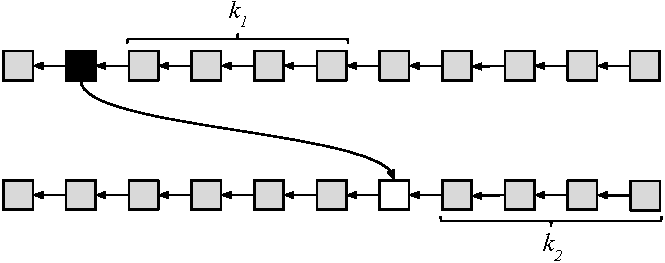
\includegraphics[width=0.7 \columnwidth,keepaspectratio]{chapters/sidechains/figures/events.pdf}
    \label{fig.events}
    \vspace{-2em}
\end{figure}

While the motivation for the construction is to be able to move assets from one
blockchain to another, we generalize the notion of sidechains from this strict
setting. In general, we would like the target blockchain to be able to react to
any \emph{event} that occurs on the source blockchain. Such events can be the
fact that a transaction with a particular \textsc{txid} took place, that a
certain account was paid a certain amount of money, or that a particular smart
contract was instantiated. Our sidechain construction allows the target
blockchain to react to events that took place on the source blockchain. This
reaction can be implemented in its target blockchain smart contracts. We
describe our construction in pseudocode similar to Ethereum' \emph{Solidity}. In
Solidity, \emph{events} can be fired arbitrarily from within a smart contract
and do not have a semantic interpretation. In this setting, events are defined
by Solidity using the \textsf{event} type and have an \emph{event name}, a
\emph{contract address} which fired them, as well as certain parameter values. A
contract can elect to fire an event with any name and any parameters of its
choice by invoking the \textsc{emit} command.

A high-level overview of cross-chain event transmission is shown in
Figure~\ref{fig.events}. The process is as follows. First, an event is fired in
the source blockchain, shown at the top. This could be any event that can be
emitted using Ethereum's \textsc{emit} command. This event firing is caused by a
certain transaction which is included at a certain block, indicated in black at
the top. This block is then buried under $k_1$ subsequent blocks within the
source blockchain, where the $k_1$ parameter is a security parameter of the
scheme depending on the specific parameters of the source
blockchain~\cite{backbone}. As soon as this confirmation occurs, the
target blockchain can react to the event, shown at the bottom. This reaction
occurs in a transaction which is included in a block within the target
blockchain, illustrated in white. As usual, the block needs to be confirmed by
waiting for $k_2$ blocks to be mined on top of it. It is possible that $k_1 \neq
k_2$ because of different blockchain parameters such as a difference in block
generation time or network synchrony.
In this figure, arrows between blocks of
the same blockchain indicate authenticated ancestry. The arrow between the two
blockchains indicates the data transfer needed for the event.

Using this basic functionality of event information exchange between
blockchains, we can construct two-way pegged sidechains. In such a construction,
an asset that exists on one blockchain will gain the ability to be \emph{moved}
to a different blockchain and back. We will use the example of moving ether, the
native asset of the Ethereum blockchain, from the Ethereum blockchain into the
Ethereum Classic blockchain and back. Such an action is different from
\emph{exchanging} ether (ETH), the native token of the Ethereum blockchain, with
ether classic (ETC), the native token of the Ethereum Classic blockchain.
Instead, the asset retains its nature; it maintains its price and its ability to
be used for the same purposes, while being governed by the rules of the new
blockchain, such as different performance, fees, features, or  security
guarantees. Furthermore, no counterparty or market is required to perform the
exchange; the transfer is something a party can do on its own.

\section{Smart Contract Construction}

\todo{Clean up this section}

\subsection*{Cross-chain certificates}
For our construction, we use a primitive called Non-Interactive Proofs of
Proof-of-Work recently introduced in~\cite{nipopows}.
Non-Interactive Proofs of Proofs-of-Work are cryptographic protocols which
implement a \emph{prover} and a \emph{verifier}. The prover is a \emph{full
node} on the \emph{source blockchain}. The verifier does not have access to
that blockchain, but knows the source genesis block $\mathcal{G}$. The prover
wants to convince the verifier that an \emph{event} took place in the source
blockchain; for instance, a smart contract method was called with certain
parameters or that a payment was made into a particular address. Whether such an
event took place can easily be determined if one inspects the whole blockchain.
However, the prover wishes to convince the verifier by only sending a
\emph{succinct proof}, a short string which does not grow linearly  with the
size of the source blockchain, but, rather, \emph{polylogarithmically}. The
verifier must not be fooled by \emph{adversarial provers} who provide incorrect
proofs claiming that an event happened while in fact it didn't, or that it
didn't while in fact it did. These adversaries can also mine blocks, but the
honest parties are assumed to control the majority of computational power on
both the source and the target blockchain networks. To withstand such attacks,
the verifier accepts multiple proofs, at least one of which is assumed to have
been honestly generated (this assumption is necessary in standard blockchain
protocols in general~\cite{EPRINT:KKZG15,wust2016ethereum}). Comparing these
proofs against each other, the verifier extracts a reliable truth value
corresponding to the same value it would deduce if it were to be running a full
node on the blockchain itself. This property is the \emph{security} of NIPoPoWs
proven in~\cite{nipopows}.

The NIPoPoWs construction talks about \emph{predicates} evaluated on
blockchains, but we are interested in \emph{events}. We can translate from
events to predicates provable with NIPoPoWs. Specifically, given a genesis block
$\mathcal{G}$, a smart contract address \textsf{addr}, an event name
\textsf{Event}, and a series of event parameter values $(\textsf{param}_1,
\textsf{param}_2, \cdots, \textsf{param}_n)$, the predicate $e$ we wish to check
for truth is the following: \emph{Has the event named \textsf{Event} been fired
with parameters $(\textsf{param}_1, \textsf{param}_2, \cdots, \textsf{param}_n)$
by the smart contract residing in address \textsf{addr} on the blockchain with
genesis block $\mathcal{G}$ at least $k$ blocks ago?} This predicate
is (1) \emph{monotonic}, meaning that it starts with the value \textsf{false}
and, if it ever becomes \textsf{true}, it cannot ever change its value back as
the blockchain grows; (2) \emph{infix-sensitive}, meaning that its truth value
can be deduced by inspecting a polylogarithmically-bound number of blocks on the
blockchain (in our case one block, within which the event firing was confirmed);
and (3) \emph{stable}, meaning that, if one party deduces that its value is
\textsf{true}, then soon enough \emph{all} parties will deduce that its value is
\textsf{true}. This last property stems from the requirement that the event be
buried under $k$ blocks ensuring a blockchain reorganization up to $k$ blocks
ago cannot affect the predicate's value.

In order to determine whether an event took place, the NIPoPoW verifier function
\textsf{verify}$^{\mathcal{G},e}_{k,m}(\mathcal{P})$ accepts the event
description in the form of a blockchain predicate $e$, which we gave above, the
genesis block of the remote chain $\mathcal{G}$, as well as two security
parameters $k$ and $m$. These security parameters can be constants specified
when the sidechain system is created (concrete values for these are given
in~\cite{nipopows}). Subsequently, the NIPoPoW verifier accepts a set of
\emph{proofs} $\mathcal{P} = \{\pi_1, \pi_2, \cdots, \pi_n\}$ which it compares
and extracts a truth value for the predicate: Whether the event has taken place
in the remote blockchain or not. As long as at least one \emph{honestly
generated} proof $\pi_i$ is provided, the verifier's security ensures that the
output will correspond to whether the event actually occurred.

Our protocol works as follows. Whenever an event of interest occurs on the
source blockchain, the occurence of this event is observed by a source
blockchain honest node, who generates a NIPoPoW about it. The target blockchain
contains a smart contract with a method to accept and verify the veracity of
this proof. The node can then submit the proof to the smart contract by
broadcasting a transaction on the target blockchain. As soon as the proof is
validated by the smart contract, the target blockchain can elect to react to the
event as desired.

\noindent
\textbf{Adoption considerations. } Our construction has certain prerequisites
for both the source and the target blockchain before it can be adopted. In the
case of bidirectionally connected blockchains, both of them must satisfy the
source and the target blockchain prerequisites.

\begin{itemize}
  \item \textbf{The source blockchain} needs to support \emph{proofs} about it,
        which requires augmenting it with an \emph{interlink} vector, the
        details of which can be found in~\cite{popow}. This interlink vector
        can be added to a blockchain using a \emph{user-activated velvet
        fork}~\cite{nipopows,velvet}, which is performed without miner awareness
        and does not require a hard or soft fork. However, only events occuring
        \emph{after} the velvet fork can be proven. New blockchains can adopt
        this from genesis.
  \item \textbf{The target blockchain} needs to be able to run the above
        \textsf{verify} function. This function can be programmed in a
        Turing-complete language such as Solidity. If the source blockchain
        proof-of-work hash function is available as an opcode or pre-compiled
        smart contract within the target blockchain's VM the way, e.g.,
        Bitcoin's SHA256 hash function is available in Solidity, the
        implementation can be more gas-efficient.
\end{itemize}

\noindent
\textbf{Blockchain agnosticism. }
We underline the remarkable property that miners and full nodes of the target
blockchain do not need to be aware of the source blockchain at all. To them,
all information about the source blockchain is simply a string which is passed
as a parameter to a smart contract and can remain \emph{agnostic} to its
semantics as a proof. Additionally, miners and full nodes of the source
blockchain do not need to be aware of the target blockchain. Only the parties
interested in facilitating cross-chain events must be aware of both. Those
untrusted facilitators need to maintain an SPV node on the source blockchain
about which they generate their NIPoPoW. To broadcast their proof on the target
blockchain, they connect to target blockchain nodes and send the transaction
containing the NIPoPoW. Blockchain agnosticism allows users to initiate
cross-chain relationships between different blockchains \emph{dynamically}, as
long as the blockchains in question satisfy the above prerequisites.

\subsection*{Cross-chain events}

We give our \textsf{crosschain} construction in Algorithm~\ref{alg.crosschain}.
Initially, our communication will be unidirectional. In the next section, we
use two unidirectional channels to establish bidirectional communication. This
smart contract runs on the target blockchain and informs it about events that
took place in the source blockchain. It is parameterized by three parameters:
$k$ and $m$ are the underlying security parameters of the NIPoPoW protocol. The
value $z$ is a \emph{collateral} parameter, denominated in ether (or the native
currency of the blockchain in which the execution takes place) and is used to
incentivize honest participants to intervene in cases of false claims. The
contract utilizes the NIPoPoW \textsf{verify} function parameterized by the
event $e$, the remote genesis block $\mathcal{G}$ and the security parameters
$k$ and $m$. We do not give an explicit implementation of \textsf{verify}, as it
can be implemented in a straightforward manner by translating the pseudocode
listing of~\cite{nipopows}. For our purposes, it suffices to treat it as a black
box which, given a set of proofs, at least one of which is honestly generated,
returns the truth value of the respective predicate.

\import{./}{chapters/sidechains/algorithms/alg.crosschain.tex}

The contract allows detecting remote blockchain events and can be \emph{inherited}
by other contracts that wish to adopt its functionality. It works as follows.
First, the \textsf{initialize} method is called exactly once to configure the
contract, passing the \emph{hash} of the genesis block of the remote chain which
this contract will handle. This method is \textsf{internal} and can only be
called by the contract inheriting from it. Users of the contract can check  it
has been configured with the correct genesis block prior to using it. We note
that, while our algorithm does not reflect this to keep complexity low, it is
possible to have a contract interact with \emph{multiple} remote chains by
extending it to include multiple geneses.

The lifecycle of an event submission is illustrated in
Figure~\ref{fig.sequence}. When an event has taken place in the source
blockchain, any source blockchain SPV node, the \emph{author}, can inform the
\textsf{crosschain} contract about this fact by generating a NIPoPoW $\pi$
claiming that the event took place based on their current view of the source
blockchain. This proof can then be submitted to the target blockchain by calling
the \textsf{submit-event-proof} function and passing it the proof $\pi$ and the
event predicate $e$. The submission is accompanied by a collateral payment $z$.
If the author is honest, this collateral will be returned to her later. The
\textsf{submit-event-proof} function runs the NIPoPoW \textsf{verify} algorithm
to check that the proof $\pi$ is well-formed and that it claims that the
predicate is \textsf{true}. It then stores the proof for later use. It also
stores the address of the \emph{author} and an \emph{expiration block number}.

\begin{figure}[H]
    \caption{A sequence diagram showing the actions of the untrusted SPV node
             when communicating with both blockchain networks and the lifecycle
             of an event submission}
    \centering
    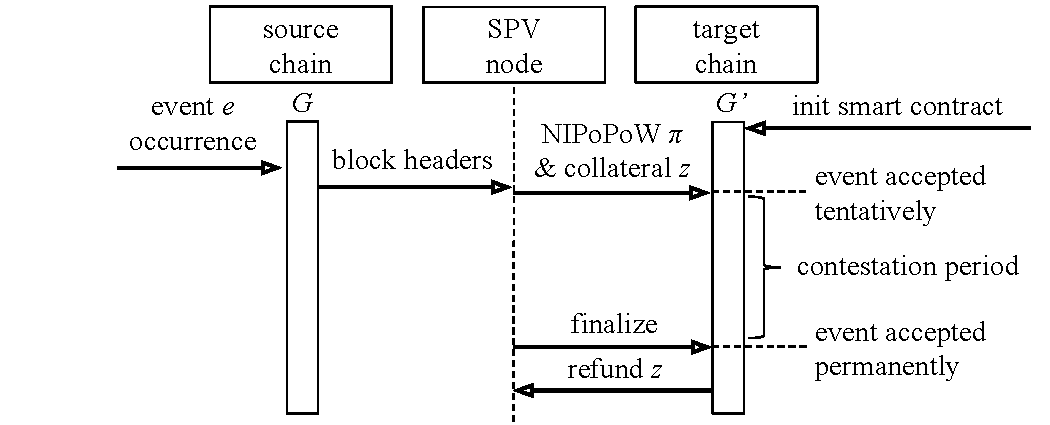
\includegraphics[width=0.9 \columnwidth,keepaspectratio]{chapters/sidechains/figures/sequence-diagram.pdf}
    \label{fig.sequence}
\end{figure}

Upon submission of a proof to the \textsf{submit-event-proof} function, the
event is \emph{tentatively accepted} for a \emph{contestation period} of $k$
blocks, during which any other party, the \emph{contester}, can provide a
counter-proof showing that the original proof was fraudulent. The contester can
call the \textsf{submit-contesting-proof} function passing it the contesting
proof $\pi^*$ and the event predicate $e$. The function runs the NIPoPoW
\textsf{verify} algorithm to compare the original proof
$\textsf{events}[e].\textsf{proof}$ against the contesting proof $\pi^*$. If the
verification algorithm concludes that the original proof was fraudulent, the
tentatively accepted event is abandoned and the collateral is paid to the
contester.

Otherwise, when the contestation period has expired without any valid
contestations, the author can call the \textsf{finalize-event} function. This
function changes the acceptance of the event from tentative to \emph{permanent}
by including it in the \textsf{finalized-events} set and returns the collateral
to the author. Finally, the \textsf{event-exists} function can be used by the
inheriting contract to check if an event has been permanently accepted. The
target blockchain state during this execution is shown in
Figure~\ref{fig.contestation}. The source blockchain's event included in the
black box, upon sufficient confirmation by $k_1$ blocks (not shown), is
transmitted to the target blockchain at the bottom. The target blockchain
includes the event \emph{tentatively} in block $1$ until a contestation period
of $k_2$ has passed; the event is included \emph{permanently} in block $2$;
subsequently, permanent inclusion needs to be confirmed with $k_2$ further
blocks.

\begin{figure}[H]
    \caption{The target blockchain state during event submission}
    \centering
    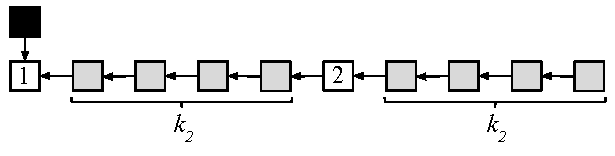
\includegraphics[width=0.6 \columnwidth,keepaspectratio]{chapters/sidechains/figures/contestation.pdf}
    \label{fig.contestation}
\end{figure}

\subsection*{Two-way pegged sidechains}
Having created the generic crosschain contract, we now build two-way pegged
sidechains on top. For concreteness, we use the example of transferring ether
(ETH), the native currency of the Ethereum blockchain, to the Ethereum Classic
blockchain, and back. We note that this example is arbitrary and for
illustration. Our construction can be used between any work-based blockchains
satisfying the prerequisites detailed above.

When ether is moved to the Ethereum Classic blockchain, it will be represented
as an ERC20 token\footnote{The ERC20 standard~\cite{erc20} defines an interface
implementable by smart contracts that enables holding and transferring custom
fungible tokens such as ICO tokens.} within Ethereum Classic. Let this custom
token be called ETH20. The asset retains its nature as it moves from one
blockchain to another if it is always possible to move ETH into ETH20 and back
at a one-to-one rate. The economic reason is that the price of ETH and ETH20 on
the market will necessarily be the same. If the price of ETH were to ever be
significantly above the price of ETH20 in the market, then a rational
participant would exchange their ETH20 for ETH using sidechains and sell their
ETH on the market instead, and vice versa. There can be a small discrepancy in
the two prices which stems from two different factors: First, the fees needed
for a cross-chain transfer; and second, the temporary market fluctuations that
can occur during the limited time needed to perform the cross chain transfer
($k_1 + 2k_2$). If we assume the price fluctuation (of ETH20 denominated in ETH)
per unit of time is bounded, then the market price difference between ETH and
ETH20 at any moment in time can be bounded by the sum of these two factors.

The sidechain smart contracts are presented in Algorithm~\ref{alg.sidechain}.
These smart contracts both extend the \textsf{crosschain} smart contract of
Algorithm~\ref{alg.crosschain}. Furthermore, \textsf{sidechain}$_2$ also
inherits basic \textsf{ERC20} functionality which allows token owners to
transfer the token~\cite{openzeppelin-erc20}. The \textsf{sidechain}$_1$
contract will be instantiated on Ethereum, while the \textsf{sidechain}$_2$
contract will be instantiated on Ethereum Classic. Suppose the genesis block
hash of Ethereum is $\mathcal{G}_1$ and of Ethereum Classic is $\mathcal{G}_2$.
We will use the genesis block hash of each blockchain as its unique identifier.

The two smart contracts both contain an \textsf{initialize} method which accepts
the hash of the remote blockchain as well as the address of the remote smart
contract it will interface with. Note that, while the two genesis hashes can be
hard-coded into the respective smart contract code itself, the remote contract
address cannot be built-in as a constant into the smart contract, but must be
later specified by calling the \textsf{initialize} function. The reason is that,
if \textsf{sidechain}$_1$ were to be created on $\mathcal{G}_1$, it would
require the address of \textsf{sidechain}$_2$ to exist prior to its creation,
and vice versa in a circular dependency. Therefore, the two contracts must first
be created on their respective blockchain to obtain addresses, and then their
\textsf{initialize} methods can be called to inform each contract about the
address of the other. Specifically, first the contract \textsf{sidechain}$_1$ is
created on $\mathcal{G}_1$ to obtain its instance address which we also
denote \textsf{sidechain}$_1$. Then the second contract, \textsf{sidechain}$_2$,
is created on $\mathcal{G}_2$ to obtain its address \textsf{sidechain}$_2$.
Subsequently, the \textsf{initialize} function of \textsf{sidechain}$_1$ is
called, passing it $\mathcal{G}_2$ and the address \textsf{sidechain}$_2$.
Finally, \textsf{initialize} is called on \textsf{sidechain}$_2$, passing it
$\mathcal{G}_1$ and the address \textsf{sidechain}$_1$. These initialization
parameters are stored by the respective smart contracts for future use. As the
\textsf{crosschain} contract requires, the \textsf{initialize} method can only
be called once. Any user wishing to utilize this sidechain is expected to
validate that the contracts have been set up correctly and that
\textsf{initialize} has been called with the appropriate parameters.

\import{chapters/sidechains/algorithms/}{alg.sidechain-pow.tex}

\textsf{sidechain}$_1$ contains a \textsf{deposit} function
which is \emph{payable} in the native asset of Ethereum, ETH. When a user pays
ETH into the \textsf{deposit} function, the funds are held by the smart contract
and can later be used to pay parties who wish to \emph{withdraw}, an operation
performed by calling the \textsf{withdraw} function. \textsf{sidechain}$_2$
contains similar \textsf{deposit} and \textsf{withdraw} functions which,
however, do not pay in the native currency of Ethereum Classic, but instead
maintain a \textsf{balance} mapping akin to a typical ERC20 implementation. The
balance is updated when a user deposits or withdraws.

Moving funds from the Ethereum blockchain into the Ethereum Classic blockchain
works as follows. First, the user pays with ETH to call the \textsf{deposit}
function of \textsf{sidechain}$_1$ which resides on $\mathcal{G}_1$, passing the
\textsf{target} parameter which indicates their address in the Ethereum Classic
blockchain that they wish to receive the money into. This call emits an event,
\textsf{Deposited}$_1$ which contains the necessary data: the \textsf{target},
the \textsf{amount} paid, as well as a nonce \textsf{ctr} to allow for future
payments of the same amount to the same target. When the event has been emitted
and buried under $k_1$ blocks within the Ethereum blockchain, the user produces
an Ethereum NIPoPoW $\pi_1$ about the predicate $e_1$ which claims that the
event \textsf{Deposited}$_1$ has been emitted in blockchain $\mathcal{G}_1$ with
the particular parameters by the contract residing at address
\textsf{sidechain}$_1$.
% We
% will slightly abuse notation for event predicates and let $e_1$ be specified by
% the tuple containing the contract address, event name and parameters
% $(\textsf{sidechain}_1, \textsf{Deposited}_1, (\textsf{amount}, \textsf{target},
% \textsf{ctr}))$, noting that there is an obvious correspondence between the two.

Subsequently, the user calls the \textsf{submit-event-proof} function of
\textsf{sidechain}$_2$ (which is inherited from the \textsf{crosschain}
contract), passing the NIPoPoW $\pi_1$ and the event predicate $e_1$ and paying
collateral $z$, which registers $e_1$ on \textsf{sidechain}$_2$ as tentative.
Because the user is honest, no adversary can produce a $\pi^*_1$
which disproves their claim during the dispute period, and therefore the user
waits for $k_2$ blocks for the contestation period to expire without any
successful contestations. She then calls the \textsf{finalize-event} function
for $e_1$ and receives back the collateral $z$, marking the event permanent.
Finally, she calls the function \textsf{withdraw} of \textsf{sidechain}$_2$,
passing it the same parameters that $e_1$ was issued with. The \textsf{withdraw}
function checks that $e_1$ exists using the \textsf{event-exists} method, which
will return \textsf{true}. The user is then credited with \textsf{amount} in
their ETH20 balance stored in $\textsf{balances}[\textsf{target}]$. This
increment in balance creates brand new ETH20 tokens. The \textsf{withdraw}
function also stores the signature of the event parameters that have been spent
to avoid replay attacks, which is not shown here for algorithm brevity.

The user can then transfer their ETH20 tokens by utilizing the functionality
inherited from the \textsf{ERC20} contract.  When some (not necessarily the
same) user is ready to move some (not necessarily the same) amount of ETH20 from
the Ethereum Classic blockchain back into ETH on the Ethereum blockchain, they
follow the reverse procedure: They call the \textsf{withdraw}
function of \textsf{sidechain}$_2$ which ensures their ERC20 balance is
sufficient, deduces the requested amount, and fires an event $e_2$ as before. At
this point, these particular ETH20 tokens are destroyed by the balance
deduction. Once $e_2$ is confirmed in $\mathcal{G}_2$, the user produces the
NIPoPoW $\pi_2$ about $e_2$ which claims a payment was made within
$\mathcal{G}_2$. That proof is then submitted to \textsf{sidechain}$_1$ by
calling the \textsf{submit-event-proof} and \textsf{finalize-event} functions as
before. Last, the user calls the \textsf{withdraw} function of
\textsf{sidechain}$_1$, which uses the \textsf{event-exists} function which will
return \textsf{true}, finally paying back the user the respective amount of ETH.
Because the only way to create ETH20 tokens in \textsf{sidechain}$_2$ is by
depositing ETH into \textsf{sidechain}$_1$, there will always exist a sufficient
balance of ETH owned by the \textsf{sidechains}$_1$ smart contract to pay for
any requested withdrawals.

Suppose now that an adversarial user makes a false claim that an event $e$ took
place in $\mathcal{G}_1$ and posts a relevant NIPoPoW $\pi$ in $\mathcal{G}_2$.
If an honest party is monitoring the chain $\mathcal{G}_2$ for the appearance of
NIPoPoWs and the chain $\mathcal{G}_1$ for the firing of events, the fraudulence
of $\pi$ will be immediately obvious to them. They can subsequently generate a
contesting NIPoPoW $\pi^*$ providing a counter-claim that $e$ did not occur. The
honest party will broadcast this transaction at the beginning of the
contestation period. Due to the \emph{liveness} property of $\mathcal{G}_2$, the
honest party will manage to include this transaction into $\mathcal{G}_2$ within
one of the blocks before the end of the contestation period. The collateral $z$
must be sufficient to incentivize an honest party to monitor $\mathcal{G}_1$ and
$\mathcal{G}_2$ simultaneously, pay for transaction fees and ensure the time
needed to generate a NIPoPoW $\pi^*$ is small as compared to block generation
time. The argument for $\mathcal{G}_2$ is analogous.
We make this security argument formal in the next section.

\section{Security of Smart Contract Implementation}

\todo{Clean up this section}

We now formalize our protocol and provide a cryptographic analysis of its
security. As NIPoPoWs security is modelled in the Bitcoin
Backbone Protocol~\cite{backbone}, we work in the same model (and note
that the same mathematical model also captures Ethereum). We assume that the
standard results of the backbone protocol are attained, namely blockchain
\emph{persistence} and \emph{liveness}. Persistence and liveness can be proved
to hold with overwhelming probability under the honest mining majority
assumption. For the details of that result, consult the Bitcoin Backbone
paper~\cite{backbone}.

We adopt the sidechains security definition from related work on proof-of-stake
sidechains~\cite{pos-sidechains}.

We will show that proving, to the maintainers of a chain $\mathcal{G}_2$, that
an event $e$ took place in chain $\mathcal{G}_1$ without it actually happening,
can only occur if the underlying NIPoPoWs protocol is insecure. Therefore, our
proof strategy follows the standard form of a cryptographic computational
reduction. In our assumptions, we will make use of the persistence and
liveness of $\mathcal{G}_2$, but only the persistence of $\mathcal{G}_1$.

\begin{theorem}
  Assume a secure NIPoPoWs construction. Then, under the honest majority
  assumption for both $\mathcal{G}_1$ and $\mathcal{G}_2$, for all PPT
  adversaries $\mathcal{A}$ and for all environments $\mathcal{Z}$, the
  proof-of-work sidechains construction between $\mathcal{G}_1$ and
  $\mathcal{G}_2$ with contestation period $2k$ is secure, except with
  negligible probability in $k$.
\end{theorem}
\begin{proof}
  Let $\mathcal{A}$ be an arbitrary PPT adversary against the proof-of-work
  sidechains construction and $\mathcal{Z}$ be an arbitrary environment. We will
  construct an adversary $\mathcal{A}^*$ against NIPoPoWs and an environment
  $\mathcal{Z}^*$ in which it will operate.

  Suppose, without loss of generality, that $\mathcal{A}$ can break the security
  of proof-of-work sidechains during a cross-chain transfer from $\mathcal{G}_1$
  to $\mathcal{G}_2$. (Because the construction is symmetric, if the adversary
  is not able to do that, then they will be able to break the security of a
  cross-chain transfer from $\mathcal{G}_2$ to $\mathcal{G}_1$ and the proof
  follows in the same manner.)

  Note that $\mathcal{A}$ works in an environment with two blockchains,
  $\mathcal{G}_1$ and $\mathcal{G}_2$, while $\mathcal{A}^*$ must work in the
  environment of one blockchain, namely $\mathcal{G}_1$.

  % TODO: Make Z* swallow the environment of Z
  % TODO: Mention that the NIPoPoWs that we use have adaptive predicates
  % LIV_1 -> LIV_2
  $\mathcal{A}^*$ works as follows. First, it simulates the execution of the
  blockchain civilization $\mathcal{G}_2$. That is, it creates a new random
  oracle for $\mathcal{G}_2$ which is independent of its external random oracle
  used with $\mathcal{G}_1$. For any random oracle queries of $\mathcal{A}$
  pertaining to $\mathcal{G}_1$, $\mathcal{A}^*$ forwards the queries to its
  external random oracle. For random oracles queries of $\mathcal{A}$ pertaining
  to $\mathcal{G}_2$, $\mathcal{A}^*$ answers its queries with its simulated
  and independent random oracle. Because $\mathcal{A}$ is subject to honest
  majority limitations in both $\mathcal{G}_1$ and $\mathcal{G}_2$, it follows
  that $\mathcal{A}^*$ will respect honest majority with regards to its external
  random oracle. For any environment instructions requested by $\mathcal{Z}$
  pertaining to $\mathcal{G}_1$ (namely, the creation of new parties), the
  instructions are mirrored by $\mathcal{Z}^*$. Intructions of $\mathcal{Z}$
  pertaining to $\mathcal{G}_2$ are simulated by $\mathcal{A}^*$. All diffusions
  of blocks in $\mathcal{G}_1$ by $\mathcal{A}$ are also diffused by
  $\mathcal{A}^*$, while diffusions in $\mathcal{G}_2$ by $\mathcal{A}$ are held
  private.

  $\mathcal{A}^*$ monitors the chains adopted by honest parties and for every
  round $r$ observes the state of all honest parties. $\mathcal{A}^*$ looks for
  a round $r$, an event $e$, a $\mathcal{G}_1$ maintainer $p_1$ and a
  $\mathcal{G}_2$ maintainer $p_2$ for which the following properties hold:

  \begin{enumerate}
    \item $p_1$ has not included $e$ in their state
    \item $p_2$ has included $e$ in their \textsf{finalized-events} state
  \end{enumerate}

  Because of the construction of $p_2$, \textsf{finalized-events} can contain
  $e$ only if an issuance of \textsf{submit-event-proof} is included at least
  $2k$ blocks deep and contains the respective NIPoPoW $\pi$ stored in
  $\textsf{events}[e].\textsf{proof}$. $\mathcal{A}^*$ now returns the proof
  $\pi$.

  We will now analyze the probability of success of $\mathcal{A}$. Consider
  the following (probabilistic) events:

  \begin{enumerate}
    \item $\textsc{SC-Brk}$ that $\mathcal{A}$ is successful
    \item $\textsc{Cert-Brk}$ that $\mathcal{A}^*$ is successful
    \item $\textsc{Per}_1$ that persistence is maintained in $\mathcal{G}_1$
    \item $\textsc{Per}_2$ that persistence is maintained in $\mathcal{G}_2$
    \item $\textsc{Live}_2$ that liveness is maintained in $\mathcal{G}_2$
    \item $\textsc{BC}$ the union of $\textsc{Per}_1 \land \textsc{Per}_2 \land \textsc{Live}_2$
  \end{enumerate}

  From total probability we obtain:

  \[
  \Pr[\textsc{SC-Brk}] = \Pr[\textsc{SC-Brk}|\textsc{BC}]\Pr[\textsc{BC}]
                       + \Pr[\textsc{SC-Brk}|\lnot \textsc{BC}]\Pr[\lnot \textsc{BC}]
  \]

  From the honest majority assumption of $\mathcal{G}_1$, we deduce that
  $\Pr[\lnot \textsc{Per}_1]$ and $\Pr[\lnot \textsc{Live}_1]$ are negligible,
  and similarly from the honest majority assumption of $\mathcal{G}_2$ we deduce
  that $\Pr[\lnot \textsc{Per}_2]$ is negligible, therefore
  $\Pr[\lnot \textsc{BC}]$ is negligible. It now suffices to show that
  $\Pr[\textsc{SC-Brk}|\textsc{BC}]\Pr[\textsc{BC}]$ is negligible.

  Suppose that $\textsc{SC-Brk}$ occurs. It follows that a (blockchain) event
  $e$ must have been adopted by $p_2$ with some NIPoPoW $\pi$, but not by $p_1$,
  as detailed above. Suppose now that $\textsc{BC}$ occurs.

  Because of the \emph{persistence} of $\mathcal{G}_2$, when $\pi$ was burried
  under $k$ blocks in the adopted chain of $p_2$, all honest parties in
  $\mathcal{G}_2$ must have seen $\pi$ (this warrants the oldest $k$ of the $2k$
  blocks in the contestation period). Because of the \emph{liveness} of
  $\mathcal{G}_2$, at least one honest block must have been included in the last
  $k$ blocks after $\pi$ had been received by all honest parties (this warrants
  the latest $k$ of the $2k$ blocks in the contestation period).

  Because of the \emph{persistence} of $\mathcal{G}_1$, if $e$ is not included
  in the state of $p_1$ at round $r$, then therefore it cannot have been
  included in the state of any $\mathcal{G}_1$ party during round $r - \eta k$.
  It follows that an honest party will attempt and succeed in generating a
  $\mathcal{G}_2$ block containing a contesting proof $\pi^*$ attesting to the
  fraudulence of event $e$ by invoking
  $\textsf{submit-contesting-proof}(\pi^*, e)$ and this block will be adopted by
  $p_2$. As $p_2$ has finalized $e$, then therefore it must be such that
  $\textsf{verify}^{e, \mathcal{G}}_{k,m}(\{\pi, \pi^*\})$, and therefore
  \textsc{Cert-Brk} has occurred.

  Putting the above together, we obtain that:

  \[
  \Pr[\textsc{Cert-Brk}] \geq \Pr[\textsc{SC-Brk}|\textsc{BC}]\Pr[\textsc{BC}]
  \]

  From the NIPoPoW security assumption, we have that $\Pr[\textsc{Cert-Brk}]$ is
  negligible. Therefore, $\Pr[\textsc{SC-Brk}]$ is negligible.
\end{proof}

% TODO: prove correctness, i.e., that an honest user will never be disputed
% successfully by an adversary


% burn
\section{Unidirectionality with Proof-of-Burn}\label{section:sidechains:burn}
\section{Introduction}\label{section:introduction}
Since the dawn of history, humans have entertained the defiant thought of money
burning, sometimes literally, for purposes ranging from artistic effect~\cite{kfoundation} to
protest~\cite{armchair}, or to prevent it from falling into the hands of pirates~\cite{laertiuslives,ciceroinventione}.
People did not shy away from the practice in the era of cryptocurrencies.
Acts of money burning immediately followed the inception of Bitcoin~\cite{bitcoin} in 2009,
with the first recorded instance of intentional cryptocurrency destruction
taking place on August 2010~\cite{interesting-address}, a short three months after the first real-world
transaction involving cryptocurrency in May 2010~\cite{SP:BMCNKF15}. For the first time, however,
cryptocurrencies exhibit the unique ability for money burning to be provable
retroactively in a so-called \emph{proof-of-burn}.

First proposed by Iain
Stewart in 2012~\cite{stewart}, proof-of-burn constitutes a mechanism for the
destruction of cryptocurrency irrevocably and provably.
The ability to create convincing proofs changed the practice of money burning
from a fringe act to a rational and potentially useful endeavour. It has since
been discovered that metadata of the user's choice can be uniquely ascribed to
an act of burning, allowing each burn to become tailored to a particular
purpose. Such protocols have been used as a consensus mechanism similar to
proof-of-stake (Slimcoin~\cite{slimcoin}), as a mechanism for establishing
identity (OpenBazaar~\cite{openbazaarreputationpledges,zindros2016trust}), and for notarization (Carbon
dating~\cite{clark2012commitcoin} and
OpenTimestamps~\cite{todd2016opentimestamps}). A particularly apt use case is
the destruction of one type of cryptocurrency to create another. In one
prolific case, users destroyed more than $2{,}130.87$ BTC ($\$1.7$M at the
time, $\$21.6$M in today's prices) for the bootstrapping of the
Counterparty cryptocurrency~\cite{counterparty}.

While its adoption is undeniable, there has not been a formal treatment for
proof-of-burn. This is the gap this work aims to fill.

\noindent
\textbf{Our contributions.}
A summary of our contributions is as follows:
\begin{enumerate}[wide, labelwidth=!, labelindent=0pt, label=(\roman*)]
    \item \textbf{Primitive definition.} Our definitional contribution introduces proof-of-burn as a cryptographic primitive for the first time. We
    define it as a protocol which consists of two algorithms, a burn address \emph{generator} and a burn address \emph{verifier}. We put forth the foundational properties which make for secure burn protocols, namely \emph{unspendability}, \emph{binding}, and \emph{uncensorability}.   One of the critical  features of our formalization is that a tag has to be bound cryptographically with any proof-of-burn operation.
    \item \textbf{Novel construction.} We propose a novel and simple construction which is flexible and can be adapted for use in existing cryptocurrencies, as long as they use public key hashes for address generation. To our knowledge, all popular cryptocurrencies are
    compatible with our scheme. We prove our construction secure in the Random Oracle model~\cite{CCS:BelRog93}.
    \item \textbf{Bootstrapping mechanism.} We propose a cryptocurrency proof-of-burn bootstrapping mechanism which does not require miners to connect to external blockchain networks. Our mechanism in principle allows burning from any proof-of-work-based cryptocurrency.
    \item \textbf{Experimental results.} We provide a compehensively tested production grade implementation of the bootstrapping mechanism in Ethereum
    written in Solidity, which we release as open source software. Our implementation can be used to consume proofs of burn of a source blockchain
    within a target blockchain. We provide experimental measurements for the cost of burn verification and find that, in current Ethereum prices,
    burn verification costs $\$0.28$ per transaction.
    This allows coins burned on one blockchain to be consumed on another for the purposes of, for example, ERC-20 tokens creation~\cite{erc20}.
\end{enumerate}

\noindent
\textbf{Workflow.}
A user who wishes to burn her coins generates an address which we call a \emph{burn address}.
This address encodes some user-chosen metadata called the \emph{tag}. She then proceeds to send any amount of cryptocurrency to the burn address. After burning her cryptocurrency, she proves to any interested party that she irrevocably destroyed the cryptocurrency in question.

\noindent
\textbf{Properties.}
We define the following properties for a proof-of-burn protocol:
\begin{itemize}
    \item \textbf{Unspendability.} No one can spend the burned cryptocurrency.
    \item \textbf{Binding.} The burn commits only to a single tag.
    \item \textbf{Uncensorability.} Miners who do not agree with the scheme cannot censor burn transactions.
\end{itemize}

Finally, we consider the \emph{usability} of a proof-of-burn protocol important: whether a user is able to create a burn transaction using her regular cryptocurrency wallet.

\noindent
\textbf{Notation.} We use $\uniform(S)$ to denote the uniform distribution
obtained by sampling any item of the finite set $S$ with probability $\frac{1}{|S|}$.
We denote the support of a distribution $\mathcal{D}$ by $[\mathcal{D}]$. We also use $[n]$ to denote the set of integers from $1$ to $n$.
We denote the empty string by $\epsilon$ and string concatenation by $\conc$.

\section{Defining Proof-of-Burn}

Let $\kappa$ be the security parameter.

\begin{definition}[Burn protocol]
  A \emph{burn} protocol $\Pi$ consists of two functions $\GenBurnAddr(1^\kappa, t)$ and $\BurnVerify(1^\kappa, t, \burnAddr)$ which work as follows:

  \begin{itemize}
    \item $\GenBurnAddr(1^\kappa, t)$: Given a tag $t$, generate a \emph{burn address}.

    \item $\BurnVerify(1^\kappa, t, \burnAddr)$: Given a tag $t$ and an address $\burnAddr$, return $\sf{true}$ if and only if $\burnAddr$ is a burn address and correctly encodes $t$.
  \end{itemize}
\end{definition}

The protocol works as follows. Alice first generates an address $\burnAddr$ to which she sends some cryptocurrency. The address encodes information contained in a tag $t$ and is generated by invoking $\GenBurnAddr(1^\kappa, t)$. When the transaction is completed, she gives the transaction and tag to Bob who invokes $\BurnVerify(1^\kappa, t, \burnAddr)$ to verify she irrevocably destroyed the cryptocurrency while committing to the provided tag.

We require that the burn scheme is \emph{correct}.

\begin{definition}[Correctness]
  A burn protocol $\Pi$ is \emph{correct} if for all $t \in \{0,1\}^*$ and for all $\kappa \in \mathbb{N}$ it holds that
  $\BurnVerify(1^\kappa, t, \GenBurnAddr(1^\kappa, t)) = \true$.
\end{definition}

With foresight, we remark that the implementation of $\GenBurnAddr$ and $\BurnVerify$ will typically be deterministic, which alleviates the need for a probabilistic correctness definition.

Naturally, for $\GenBurnAddr$ to generate addresses that ``look'' valid but are unspendable according to the blockchain protocol requires that the burn protocol respects its format. We abstract the address generation and spending verification of the given system into a \emph{blockchain address protocol}:

\begin{definition}[Blockchain address protocol]
  A \emph{blockchain address protocol} $\Pi_\alpha$ consists of two functions $\GenAddr$ and $\sf{SpendVerify}$:

  \begin{itemize}
    \item $\GenAddr(1^\kappa)$: Returns a tuple $(\sf{pk}, \sf{sk})$, denoting the cryptocurrency address $\sf{pk}$ (a public key) used to receive money and its respective secret key $\sf{sk}$ which allows spending from that address.

    \item $\sf{SpendVerify}(m, \sigma, pk)$: Returns $\sf{true}$ if the transaction $m$ spending from receiving address $pk$ has been authorized by the signature $\sigma$ (by being signed by the respective private key).
  \end{itemize}
\end{definition}

We note that, while the blockchain address protocol is not part of the burn protocol, the \emph{security} properties of a burn protocol $\Pi$ will be defined \emph{with respect to} a blockchain address protocol $\Pi_\alpha$.

These two functionalities are typically implemented using a public key signature scheme and accompanied by a respective signing algorithm. The signing algorithm is irrelevant for our burn purposes, as burning entails the inability to spend. As the format of $m$ is cryptocurrency-specific, we intentionally leave it undefined. In both Bitcoin and Ethereum, $m$ corresponds to transaction data. When a new candidate transaction is received from the network, the blockchain node calls $\textsf{SpendVerify}$, passing the public key $pk$, which is the address spending money incoming to the new transaction $m$, together with a signature $\sigma$, which signs $m$ and should be produced using the respective secret key.

To state that the protocol generates addresses which cannot be spent from, we introduce a game-based security definition. The unspendability game $\spendattack$ is illustrated in Algorithm~\ref{alg.spend-game}.

\import{./}{chapters/sidechains/algorithms/alg.spend-game.tex}

\begin{definition}[Unspendability]
  A burn protocol $\Pi$ is \emph{unspendable} with respect to a blockchain address protocol $\Pi_\alpha$ if
  for all probabilistic polynomial-time adversaries $\mathcal{A}$ there exists a negligible function $\negl$ such that
  $
    \Pr[\spendattack_{\mathcal{A}, \Pi}(\kappa) = \textsf{true}] \leq \negl
  $.
\end{definition}

\import{./}{chapters/sidechains/algorithms/alg.bind-game.tex}

It is desired that a burn address encodes one and only one tag. Concretely, given a burn address $\burnAddr$, $\BurnVerify(1^\kappa, t, \burnAddr)$ should only evaluate to $\true$ for a single tag $t$. The game $\bindattack$ in Algorithm~\ref{alg.bind-game} captures this property.

\begin{definition}[Binding]
  A burn protocol $\Pi$ is \emph{binding} if
  for all probabilistic polynomial-time adversaries $\mathcal{A}$ there is a
  negligible function $\negl$ such that
  $\Pr[\bindattack_{\mathcal{A},\Pi}(\kappa)] \leq \negl$.
\end{definition}

We note here that the correctness and binding properties of a burn protocol are irrespective of the blockchain address protocol it was designed for.

We are now ready to define what constitutes a \emph{secure proof-of-burn protocol}.

\begin{definition}[Security]
  Let $\Pi$ be a correct burn protocol. We say $\Pi$ is \emph{secure} with respect to a blockchain address protocol $\Pi_\alpha$ if it is \emph{unspendable} and \emph{binding} with respect to $\Pi_\alpha$.
\end{definition}

The aforementioned properties form a good basis for a burn protocol. We observe that it may be possible to detect whether an address is a burn address. While this is desirable in certain circumstances, it allows miners to censor burn transactions. To mitigate this, we propose \emph{uncensorability}, a property which mandates that a burn address is indistinguishable from a regular address if its tag is not known. During the execution of protocols which satisfy this property, when the burn transaction appears on the network, only the user who performed the burn knows that it constitutes a burn transaction prior to revealing the tag. Naturally, as soon as the tag is revealed, \emph{correctness} mandates that the burn transaction becomes verifiable.

\begin{definition}[Uncensorability]
  Let $\mathcal{T}$ be a distribution of tags.
  A burn protocol $\Pi$ is \emph{uncensorable} if
  the distribution ensembles $\{(pk, sk) \gets \GenAddr(1^\kappa); pk\}_\kappa$ and
  $\{t \gets \mathcal{T}; pk \gets \GenBurnAddr(1^\kappa, t); pk\}_\kappa$ are computationally indistinguishable.
\end{definition}

\subsection{Construction}\label{sec:construction}
We now present our construction for an uncensorable proof-of-burn protocol. To generate a burn address, the tag $t$ is hashed and a perturbation is performed on the hash by toggling the last bit.
Verifying a burn address $\burnAddr$ encodes a certain tag $t$ is achieved by invoking $\GenBurnAddr$ with tag $t$ and checking whether the result matches $\burnAddr$. If it matches, the $\burnAddr$ correctly encodes $t$. Our construction is illustrated in Algorithm~\ref{alg.construction-ro}.

\import{./}{chapters/sidechains/algorithms/alg.construction-ro.tex}

We outline the blockchain address protocol for Bitcoin Pay to Public Key Hash (P2PKH)~\cite{bitcoin-dev-guide}, with respect to which we prove our construction secure and uncensorable in Section~\ref{sec:analysis}. It is parametrized by a secure signature scheme $S$ and a hash function $H$ (for completeness, we give a construction which includes the concrete hash
functions and checksums of Bitcoin in Appendix~\ref{sec.real}).
$\GenAddr$ uses $S$ to generate a keypair and hashes the public key to generate the public key hash. A tuple consisting of the public key hash and the secret key is returned.
$\SpendVerify$ takes a spending transaction $m$, a scriptSig $\sigma$ and a public key hash $pkh$. The scriptSig should contain the public key $pk$ corresponding to $pkh$ such that $H(pk) = pkh$ and a valid signature $\sigma'$ for the spending transaction $m$~\cite{bitcoin-dev-guide}. If these conditions are met, the function returns $\true$, otherwise it returns $\false$.
The blockchain address protocol is illustrated in Algorithm~\ref{alg.p2pkh}.

\import{./}{chapters/sidechains/algorithms/alg.p2pkh.tex}

\section{Comparison}

We now compare alternatives for proof-of-burn proposed in previous work. Our burn primitive captures all of these schemes.

\newcommand{\opreturn}{\texttt{OP\_RETURN}}

\noindent
\textbf{$\opreturn$.}
Bitcoin provides a native opcode called  $\opreturn$~\cite{bartoletti2017analysis} which can be used for burning.
Unfortunately,
standard wallets do not provide a user friendly interface for creating $\opreturn$ transactions.
However, it benefits the Bitcoin network by allowing the UTXO to be pruned, at
the cost of not being uncensorable.
Similarly to $\opreturn$, any provably failing Bitcoin script can be used for
burning~\cite{stewart}.

\noindent
\textbf{P2SH $\opreturn$.}
An $\opreturn$ or other provably failing script can also be used as the redeemScript for a Pay to Script Hash (P2SH)~\cite{p2sh} address. It is unspendable since there is no scriptSig that could make the script succeed. Additionally, it is uncensorable if the tag is not revealed. Finally, the scheme is user friendly since any regular wallet can create a burn transaction.

\noindent
\textbf{Nothing-up-my-sleeve.}
An address is manually crafted, so that it is clear it was not generated from a regular keypair. For example, the all-zeros address is considered nothing-up-my-sleeve\footnote{The Bitcoin address \texttt{1111111111111111111114oLvT2} encodes the all-zeros string and has received more than $50{,}000$ transactions dating back to Aug 2010.}. It is hard to obtain a public key hashing to this address, thus funds sent to it are unspendable. Because no metadata can be associated with such a burn, this scheme is not binding.

We compare the aforementioned schemes on whether they satisfy the burn protocol properties we define: Binding, unspendability and uncensorability. Additionally, we compare them based on how easily they translate to multiple cryptocurrencies. For instance, $\opreturn$ and P2SH $\opreturn$ rely on Bitcoin Script semantics and do not directly apply to any non-Bitcoin based cryptocurrencies like Monero~\cite{van2013cryptonote}, thus we say they are not \emph{flexible}. The comparison is illustrated on Table~\ref{table:comparison}.

\begin{table}[h!]
    \newcommand{\y}{$\bullet$}
    \newcommand{\n}{}
    \centering
    \caption{Comparison between proof-of-burn schemes.\label{table:comparison}}

    \begin{tabular}{ |r|c|c|c|c|c| }
     \hline
                                        & Binding & Flexible & Unspendable & Uncensorable & User friendly \\
     \hline
     $\opreturn$                        & \y      & \n       & \y          & \n & \n \\
     P2SH $\opreturn$                   & \y      & \n       & \y          & \y & \y \\
     Nothing-up-my-sleeve               & \n      & \y       & \y          & \y & \y \\
     $a \xor 1$ \textbf{(this work)}    & \y      & \y       & \y          & \y & \y \\
     \hline
    \end{tabular}
\end{table}

\subsection{Security of Burn}\label{sec:analysis}

We now move on to the analysis of our scheme. As the scheme is deterministic,
its correctness is straightforward to show.

\begin{theorem}[Correctness]
  The proof-of-burn protocol $\Pi$ of Section~\ref{sec:construction-burn} is \emph{correct}.
\end{theorem}
\begin{proof}
  Based on Algorithm~\ref{alg.construction-ro}, $\BurnVerify(1^\kappa, t, \GenBurnAddr(1^\kappa, t)) = \textsf{true}$ if and only if $\GenBurnAddr(1^\kappa, t) = \GenBurnAddr(1^\kappa, t)$, which always holds as $\GenBurnAddr$ is deterministic.
\end{proof}

We now state a simple lemma pertaining to the distribution of Random Oracle
outputs.

\begin{restatable}[Perturbation]{lem}{restateLemPerturbation}
  \label{lem.perturbation}
  Let $p(\kappa)$ be a polynomial and
  $F: \{0,1\}^\kappa \longrightarrow \{0,1\}^\kappa$ be a permutation.
  Consider the process which samples $p(\kappa)$ strings $s_1, s_2, \dots, s_{p(\kappa)}$ uniformly at random from the set $\{0, 1\}^\kappa$. The probability that there exists $i \neq j$ such that $s_i = F(s_j)$ is negligible in $\kappa$.
\end{restatable}

We will now apply the above lemma to show that our scheme is unspenable.

\begin{theorem}[Unspendability]
  If $H$ is a \emph{Random Oracle}, then the protocol $\Pi$ of Section~\ref{sec:construction-burn} is \emph{unspendable}.
\end{theorem}
\begin{proof}
  Let $\mathcal{A}$ be an arbitrary probabilistic polynomial time $\spendattack$ adversary.
  $\mathcal{A}$ makes at most a polynomial number of queries $p(\kappa)$ to the Random Oracle.
  Let $\textsc{Match}$ denote the event
  that there exist $i \neq j$ with $s_i = F(s_j)$ where $F(s) = s \xor 1$.

  If the adversary is successful then it has presented $t, pk, pkh$ such that $H(pk) = pkh$ and $H(t) \xor 1 = pkh$.
  Observe that $\spendattack_{\mathcal{A}, \Pi}(\kappa) = \true \Rightarrow \textsc{Match}$.
  Therefore $\Pr[\spendattack_{\mathcal{A}, \Pi}(\kappa)] \leq Pr[\textsc{Match}]$. Apply Lemma~\ref{lem.perturbation} on $F$
  to obtain
  $\Pr[\spendattack_{\mathcal{A}, \Pi}(\kappa)] \leq \negl$.
\end{proof}

We note that the security of the signature scheme is not needed to prove unspendability. Were the signature scheme of the underlying cryptocurrency ever found to be \emph{forgeable}, the coins burned through our scheme would remain unspendable. We additionally remark that the
choice of the permutation $F(x) = x \xor 1$ is arbitrary. Any one-to-one
function beyond the identity function would work equally well.

\noindent
\textbf{Preventing proof-of-burn.}
It is possible for a cryptocurrency to prevent proof-of-burn by requiring every address to be accompanied by a proof of possession~\cite{pop}. To the best of our knowledge, no cryptocurrency features this.

Next, our binding theorem only requires that the hash function used is collision
resistant and is in the standard model.

\import{./}{chapters/sidechains/algorithms/alg.collision-adversary.tex}

\begin{theorem}[Binding]
  If $H$ is a \emph{collision resistant} hash function then the protocol of Section~\ref{sec:construction-burn} is \emph{binding}.
\end{theorem}
\begin{proof}
  Let $\mathcal{A}$ be an arbitrary adversary against $\Pi$.
  We will construct the Collision Resistance adversary $\mathcal{A}^*$ against $H$.

  The collision resistance adversary, illustrated in Algorithm~\ref{alg.collision-adversary}, calls $\mathcal{A}$ and obtains two outputs, $t$ and $t'$. If $\mathcal{A}$ is successful then $t \neq t'$ and $H(t) \xor 1 = H(t') \xor 1$. Therefore $H(t) = H(t')$.

  We thus conclude that $\mathcal{A^*}$ is successful in the $\collisionattack$ game if and only if $\mathcal{A}$ is successful in the $\bindattack$ game.

  \[
    \Pr[\bindattack_{\mathcal{A},\Pi}(\kappa) = \true]
    =
    \Pr[\collisionattack_{\mathcal{A}^*,H}(\kappa) = \true]
  \]

  From the collision resistance of $H$ it follows that $\Pr[\collisionattack_{\mathcal{A}^*,H} = \true] < \negl$. Therefore,
  $\Pr[\bindattack_{\mathcal{A},\Pi} = \true] < \negl$, so
  the protocol $\Pi$ is binding.
\end{proof}

We now posit that no adversary can predict the public key of a secure signature scheme, except with negligible probability. We call a distribution \emph{unpredictable} if no
probabilistic polynomial-time adversary can predict its sampling. We give
the formal definition, with some of its statistical properties, in
Appendix~\ref{sec:proofs:unpred-dist}.

\begin{restatable}[Public key unpredictability]{lem}{restateLemPkUnpredictability}
  \label{lem:pk-unpredictability}
  Let $S = (\textsf{Gen}, \textsf{Sig}, \textsf{Ver})$ be a secure signature scheme.
  Then the distribution ensemble
  $X_\kappa = \{(sk, pk) \gets \textsf{Gen}(1^\kappa); pk\}$ is
  unpredictable.
\end{restatable}

The following lemma shows that the output of the random oracle is
indistinguishable from random if the input is unpredictable
(for the complete proofs see Appendix~\ref{sec:proofs:ro}).
For reference, the
definition of computational indistinguishability is included in
Appendix~\ref{sec:proofs:comp-ind}.

\begin{restatable}[Random Oracle unpredictability]{lem}{restateLemRoUnpredictability}
  \label{lem:ro-unpredictability}
  Let $\mathcal{T}$ be an unpredictable distribution ensemble and $H$ be a
  Random Oracle.
  The distribution ensemble $X = \{t \gets \mathcal{T}; H(t)\}$ is indistinguishable from
  the uniform distribution ensemble $\uniform(\{0,1\}^\kappa)$.
\end{restatable}

\begin{theorem}[Uncensorability]
  Let $S = (\Gen, \Sig, \Ver)$ be a \emph{secure signature scheme},
  $H$ be a \emph{Random Oracle},
  and $\mathcal{T}$ be an unpredictable tag distribution.
  Then the protocol of Section~\ref{sec:construction-burn} instantiated with
  $H, S, \mathcal{T}$ is \emph{uncensorable}.
\end{theorem}
\begin{proof}
  Let $X$ be the distribution ensemble of public keys generated using $\GenAddr$
  and $Y$ that of keys generated using $\GenBurnAddr$.

  From Lemma~\ref{lem:pk-unpredictability} the distribution of
  public keys generated from $S$ is unpredictable. The
  function $\GenAddr$ samples a public key from $S$ and applies the
  random oracle $H$ to it. Applying
  Lemma~\ref{lem:ro-unpredictability}, we obtain that
  $X \cind \uniform(\{0, 1\}^\kappa)$.

  The function $H'(x) = H(x) \xor 1$ is a random oracle (despite not
  being independent from the random oracle $H$).
  Since $\mathcal{T}$ is unpredictable, and
  applying Lemma~\ref{lem:ro-unpredictability} with random oracle $H'$, we
  obtain that $Y \cind \uniform(\{0, 1\}^\kappa)$.

  By transitivity, $X$ and $Y$ are computationally indistinguishable.
\end{proof}

From the above, we conclude that the tags used during the burn process must be
unpredictable. If the tag is chosen to contain a randomly generated public key
from a secure signature scheme, or its hash,
Lemmas~\ref{lem:pk-unpredictability}~and~\ref{lem:ro-unpredictability} show that
sufficient entropy exists to ensure uncensorability. Our cross-chain application
makes use of this fact.

\section{Consumption}

Over the last 5 years there has been an explosion of new cryptocurrencies. Unfortunately, it is hard for a new cryptocurrency to gain traction. Without traction, no market depth ensues and a cryptocurrency has difficulty getting listed in exchanges. But without being listed in exchanges, a cryptocurrency cannot gain traction.

This chicken-and-egg situation presents the need for a solution that circumvents exchanges and allows users to acquire the cryptocurrency directly. We propose utilizing proof-of-burn to allow users to obtain capital on a new cryptocurrency by burning a legacy cryptocurrency. We call the legacy one the \emph{source} and the new one the \emph{target cryptocurrency}, and their blockchains the \emph{source} and \emph{target blockchain} respectively. The target blockchain may support burning from multiple source blockchains.

\noindent
\textbf{Workflow.}
A user who wishes to acquire a target cryptocurrency first forms a burn address valid in the source blockchain which encodes her receiving address on the target blockchain by using it as a tag. She then sends an amount of source cryptocurrency to that address. She submits a proof of this burn to a smart contract~\cite{buterin} on the target blockchain, where it is verified and she is credited an equivalent amount of target cryptocurrency on her receiving address. Proof-of-burn verification happens in either a centralized manner which is lighter on computation, or in a decentralized manner using Non-Interactive Proofs of Proof-of-Work (NIPoPoWs)~\cite{popow,nipopows,compactsuperblocks,gtklocker}.

Target blockchain miners need not be connected to every other source blockchain network. We call this property \emph{miner-isolation} and we propose methods to achieve it.

We now describe how a smart contract on the target blockchain can verify a burn took place on the source blockchain. Note how this puts a constraint on the target blockchain to have smart contract capabilities. However there is no such constraint for the source blockchain.

In accordance to the terminology laid out in~\cite{pow-sidechains}, we call the user the \emph{prover} and the smart contract the \emph{verifier}. The prover wishes to convince the verifier that an event occurred on the source blockchain. We define an event as a simple value transfer described by a transaction id \textsf{txid}, a receiving address \textsf{addr} and an amount \textsf{amount}. Simple value transfers are supported by all cryptocurrencies, allowing a verifier to process burns from a wide range of source blockchains. Note that this event type does not yet distinguish between burn and non-burn addresses.

For a verifier to be convinced that an event occurred on a source blockchain, they ensure its transaction is contained in a stable block in the best source chain. Specifically, the following data are supplied to the smart contract as a proof:

\begin{itemize}
  \item $\tx$: The transaction which contains the burn on the source blockchain.
  \item $b$: The block header for the block which contains $\tx$.
  \item $\txInclusion$: An inclusion proof showing $\mathsf{tx} \in b$.
  \item $\blockConnection$: A proof that $b$ is contained in the best (i.e., most proof-of-work) source blockchain and is stable.
\end{itemize}

We assume the source blockchain provides a function \verifytx(\textsf{addr}, \textsf{amount}, $b$, \textsf{tx}, $\txInclusion$) which can be written in the smart contract language of the target blockchain and verifies the validity of a source blockchain transaction. It takes a source blockchain address \textsf{addr}, an amount of source cryptocurrency \textsf{amount}, a block $b$, a transaction \textsf{tx} and a proof $\txInclusion$ for the inclusion of \textsf{tx} in $b$. It returns $\true$ if \textsf{tx} contains a transfer of \textsf{amount} to \textsf{addr} and the proof $\txInclusion$ is valid for $b$.

The proof $\txInclusion$ is usually a Merkle Tree inclusion proof. More concretely, in Bitcoin, each block header contains a commitment to the set of transaction ids in the block in the form of a Merkle Tree root. Ethereum stores a similar commitment in its header --- the root of a Merkle--Patricia Trie~\cite{wood}.

For verifying that a provided block $b$ belongs to the best source blockchain and is stable, we assume the existence of a function $\textsf{in-best-chain}(b)$. We explore how it can be implemented in the ``Verifying block connection'' paragraph below.

\noindent
\textbf{Bootstraping mechanism.}
Being able to verify events, we can grant target cryptocurrency to users who burn source cryptocurrency. After burning on the source blockchain, the user calls the \textsf{claim} function with the aforementioned event and a proof for it. This function ensures that the event provided is valid and has not been claimed before (i.e. no one has been granted target cryptocurrency for this specific event in the past), that it corresponds to the transaction $\tx$ and that the block $b$ is stable, belongs to the best source chain and contains $\tx$. Then, after verifying by invoking $\BurnVerify$ that the receiving address of the event is a burn address where the tag is the function caller's address, it releases the amount of coins burned in the form of an ERC-20 token. We present the contract \textsf{burn-verifier} with this capability in Algorithm~\ref{alg.burn-verifier}.

\import{./}{chapters/sidechains/algorithms/alg.burn-verifier.tex}

In the interest of keeping this implementation generic we assume that the user receives a token in return for his burn. However, instead of minting a token, the target cryptocurrency could allow the burn verifier contract to mint native cryptocurrency for any user who successfully claims an event. This would allow the target cryptocurrency to be bootstrapped entirely though burning as desired.

\noindent
\textbf{Verifying block connection.}
We now shift our attention to the problem of verifying a block belongs in the best source chain. We provide multiple ways of implementing the aforementioned \textsf{in-best-chain} method.

\noindent
\textbf{Direct observation.}
Miners connect to the source blockchain network and have access to the best source chain. A miner can thus evaluate if a block is included in that chain and is stable. This mechanism does not provide miner-isolation. It is adopted by Counterparty.

\noindent
\textbf{NIPoPoWs.}
Verifying block connection can be achieved through NIPoPoWs, as in~\cite{pow-sidechains}.
We remark that with this setup a block connection proof may be considered valid provisionally, but there needs to be a period in which the proof can be disputed for the smart contract to be certain for the validity of the proof. Specifically, when a user performs a claim, they have to put down some collateral. If they have provided a valid NIPoPoW, a contestation period begins. Within that period a challenger can dispute the provided proof which -- provided that the dispute is successful -- would turn the result of \textsf{in-best-chain} to $\false$, abort the claim and grant the challenger the user's collateral. If the contestation period ends with the proof undisputed, then \textsf{in-best-chain} evaluates to $\true$, the collateral gets returned to the user and the claim is performed successfully.

\noindent
\textbf{Federation.}
A simpler approach is to allow a federation of $n$ nodes monitoring the source chain to vote for their view of the best source chain.

\import{./}{chapters/sidechains/algorithms/alg.in-best-chain-federation.tex}

The best source chain is expressed as the root $\mathcal{M}$ of a Merkle Tree containing the chain's stable blocks as leaves. Each federation node connects to both blockchain networks, calculates $\mathcal{M}$ and submits their vote for it every time a new source chain block is found. When a majority of $\lfloor\frac{n}{2}\rfloor + 1$ nodes agrees on the same $\mathcal{M}$, it is considered valid.

Having a valid $\mathcal{M}$, a verifier verifies a Merkle Tree inclusion proof $\blockConnection$ for $b \in \mathcal{M}$ and is certain the block provided is part of the best source chain and is stable. This approach is illustrated in Algorithm~\ref{alg.in-best-chain-federation}.

The more suitable Merkle Mountain Range~\cite{flyclient} data structure can be used to store $\mathcal{M}$ in place of regular Merkle Trees, as they constitute a more efficient append-only structure.

\subsection{Empirical Results}
In order to evaluate our consumption mechanisms, we implement the federated consumption mechanism in Solidity. We provide a concrete implementation of the \textsf{burn-verifier} contract described in Algorithm~\ref{alg.burn-verifier}. We implement the \textsf{crosschain} parent contract from~\cite{pow-sidechains}. We verify transaction data by making use of the open source bitcoin-spv library~\cite{bitcoin-spv-library}. Finally, the federation mechanism for verifying block connection is employed. The members of the federation can vote on their computed checkpoints using the \textsf{vote} function.

We release our implementation as open source software under the MIT license\footnote{\url{https://github.com/decrypto-org/burn-paper/tree/master/experiment}}.
The implementation is production-ready and fully tested with 100\% code coverage.

At the time of writing we obtain the median gas price of $6.9$ gwei and the price of Ethereum in US Dollars at $\$170.07$. The cost of gas in USD is calculated by the formula $gas * 1.173483 * 10^{-6}$ rounded to two decimal places.

\begin{center}
    \begin{tabular}{ |c|r|c| }
     \hline
     Method                         & Gas cost   & Equivalent in USD \\
     \hline
     \textsf{vote}                  & 50103 gas  & $\$0.06$ \\
     \hline
     \textsf{submit-event-proof}    & 157932 gas & $\$0.19$ \\
     \textsf{claim}                 & 78267 gas  & $\$0.09$ \\
     Total claim cost               & 262817 gas & $\$0.28$ \\
     \hline
    \end{tabular}
\end{center}

For the end user to prove an event and claim her burn, the cost is thus $\$0.28$. Comparatively, for a Bitcoin transaction to be included in the next block at the time of writing a user has to spend $\$0.77$.

\section{Deployment to Bitcoin}\label{sec.real}
\import{./}{chapters/sidechains/algorithms/alg.bitcoin-real.tex}

The scheme described above works for a generic P2PKH cryptocurrency and can be adapted to any cryptocurrency. We illustrate its suitability by giving a precise construction for Bitcoin, taking into account the engineering details that are behind the generation of a Bitcoin P2PKH address. A comparable approach can be used to generate Ethereum addresses or others.

The way Bitcoin generates P2PKH addresses is illustrated in Algorithm~\ref{alg.bitcoin-real}. Here, $\Gen$ generates an elliptic curve public key (of fixed key size $\kappa = 256$). After the elliptic curve public key is generated, it is marked by a magic number and subsequently hashed by the so-called $\BTCHASH$ algorithm, which consists of evaluating $\RIPEMD$ on the $\SHA$ of the public key. The resulting hash is additionally prefixed by a magic number indicating that the execution is taking place on the main net (and not the test net), and the final address, together with a checksum, are encoded using $\baseencode$ to obtain the final address.

Our burn algorithm follows the same structure for address generation, ensuring that the magic numbers and checksums validate correctly. In this construction, the hash function which is modelled as a random oracle is the $\BTCHASH$ algorithm. The algorithm is illustrated in Algorithm~\ref{alg.construction-real} and works as follows.
Given a tag $t$, the user derives a $160$-byte
hash $th = \RIPEMD(\SHA(t))$ which looks like a public key hash.
The least significant bit of
$th$ is then flipped to achieve unspendability. This produces the $20$-byte
\emph{perturbated hash} $th'$. The perturbated hash
is then prefixed with \texttt{0x00} to designate that we're working on the Bitcoin mainnet as usual. The checksum is calculated and appended
to it, and the result is
$\baseencode$ encoded into a Bitcoin address which correctly validates.

\import{./}{chapters/sidechains/algorithms/alg.construction-real.tex}

\subsection{Full proofs}\label{sec:proofs}

\todo{Merge these into main body in previous subsections}

In this section, we give the full proofs of our claims.
Section~\ref{sec:proofs:comp-ind} proves some facts about
computationally indistinguishable distributions. In
Section~\ref{sec:proofs:unpred-dist}, we introduce unpredictable distributions
and show that public keys are unpredictable. In Section~\ref{sec:proofs:ro},
we prove some facts about the statistical properties of random oracles,
including Lemma~\ref{lem.perturbation} from which the unspendability of our
scheme follows and Lemma~\ref{lem:ro-unpredictability} from which the
uncensorability of our scheme follows.

\subsubsection{Computational indistinguishability}\label{sec:proofs:comp-ind}

\import{./}{./chapters/sidechains/algorithms/alg.dist-game.tex}

We review the definition of computational indistinguishability between two
distributions $X$ and $Y$. Define the cryptographic game illustrated in
Algorithm~\ref{alg.dist-game}.
Computational indistinguishability mandates that no adversary can win the game,
except with negligible probability.

\begin{definition}[Computational indistinguishability]
  Two distribution ensembles $\{X_\kappa\}_{\kappa\in\mathbb{N}}$ and $\{Y_\kappa\}_{\kappa\in\mathbb{N}}$ are
  \emph{computationally indistinguishable}
  if for every probabilistic polynomial-time adversary $\mathcal{A}$,
  there exists a negligible function $\negl$ such that
  $\Pr[\distattack_{\mathcal{A},X,Y}(\kappa) = \true] < \negl$.
\end{definition}

It is clear that applying an efficiently computable function to
indistinguishable distributions preserves indistinguishability.

\import{./}{chapters/sidechains/algorithms/alg.pres-distinguisher.tex}

\begin{lemma}[Indistinguishability preservation]\label{lem:ind-pres}
  Given two
  computationally indistinguishable distribution ensembles
  $\{X_\kappa\}_{\kappa\in\mathbb{N}}$ and $\{Y_\kappa\}_{\kappa\in\mathbb{N}}$,
  let
  $\{f_\kappa\}_{\kappa\in\mathbb{N}}$,
  be an efficiently computable family of functions $X_\kappa \longrightarrow Y_\kappa$.
  Then the distribution ensembles
  $X' = \{f_\kappa(X_\kappa)\}_{\kappa\in\mathbb{N}}$
  and
  $Y' = \{f_\kappa(Y_\kappa)\}_{\kappa\in\mathbb{N}}$
  are computationally indistinguishable.
\end{lemma}
\begin{proof}
  Let $\mathcal{A}$ be a probabilistic polynomial-time distinguisher
  between $X'$ and $Y'$. Consider the probabilistic polynomial-time distinguisher $\mathcal{A}^*$ between $X$ and $Y$ illustrated in Algorithm~\ref{alg.pres-distinguisher}. Then
  $\Pr[\distattack_{\mathcal{A}^*}(\kappa) = \true] =
   \Pr[\distattack_{\mathcal{A}}(\kappa) = \true]$.
  As $\Pr[\distattack_{\mathcal{A}^*}(\kappa) = \true] \leq \frac{1}{2} + \negl$, therefore $\Pr[\distattack_{\mathcal{A}}(\kappa) = \true] \leq \frac{1}{2} + \negl$.
\end{proof}

\subsubsection{Unpredictable distributions}\label{sec:proofs:unpred-dist}

We call a distribution ensemble \emph{unpredictable} if no
polynomial-time adversary can guess its output. The cryptographic
predictability game is illustrated in Algorithm~\ref{alg.predict-game} and the
security definition is given below.

\import{.}{./chapters/sidechains/algorithms/alg.predict-game.tex}

\begin{definition}[Unpredictable distribution]
  A distribution ensemble $\{X_{\kappa}\}_{\kappa\in\mathbb{N}}$ is
  \emph{unpredictable} if for all probabilistic polynomial-time adversaries
  $\mathcal{A}$ there is a negligible function $\negl$ such that
  \[\Pr[\predict_{\mathcal{A},X}(\kappa) = \true] < \negl\,.\]
\end{definition}

We observe that, if each element of a distribution appears with negligible
probability, then the distribution must be unpredictable.

\begin{lemma}[Negligible unpredictability]\label{lem:negl-unpred}
  Consider a distribution ensemble $\{X_{\kappa}\}_{\kappa\in\mathbb{N}}$ and
  a negligible function $\negl$. If
  \[\max_{x \in [X_\kappa]}\Pr_{x^* \gets X_\kappa}[x^* = x] \leq \negl\,,\]
  then $X$ is unpredictable.
\end{lemma}
\begin{proof}
  Consider a probabilistic polynomial-time adversary $\mathcal{A}$ which
  predicts $X_\kappa$. The adversary is not given any input beyond $1^\kappa$,
  hence the distribution of its output is independent from the choice of the
  challenger. Therefore

  \begin{align*}
  \Pr[\predict_{\mathcal{A},X}(\kappa) = \true] &=
  \sum_{x' \in [X]}\Pr_{x \gets X}[\mathcal{A}(\kappa) = x'\land x = x'] =\\
  \sum_{x' \in [X]}\Pr[\mathcal{A}(\kappa) = x']\Pr_{x \gets X}[x = x']
  &\leq \negl\sum_{x' \in [X]}\Pr[\mathcal{A}(\kappa) = x']
  \leq \negl
  \,.
  \end{align*}
\end{proof}

Finally, we observe that public keys generated from secure signature schemes must
be unpredictable.

\import{./}{chapters/sidechains/algorithms/alg.forgery-adversary.tex}

\restateLemPkUnpredictability*
\begin{proof}
  Let
  $p = \max_{\widehat{pk} \in [X_\kappa]}\Pr_{pk \gets X_\kappa}[pk = \widehat{pk}]$.
  Consider the existential forgery adversary $\mathcal{A}$ illustrated in
  Algorithm~\ref{alg.forgery-adversary} which works as
  follows. It receives $pk$ as its input from the challenger, but ignores it
  and generates a new key pair $(pk', sk') \gets \textsf{Gen}(1^\kappa)$.
  Since the
  two invocations of $\textsf{Gen}$ are independent,
  \begin{align*}
    \Pr[pk = pk'] \geq \max_{\widehat{pk} \in [X_\kappa]}\Pr[pk = \widehat{pk} \land pk' = \widehat{pk}]\\
  = \max_{\widehat{pk} \in [X_\kappa]}\Pr[pk = \widehat{pk}]\Pr[pk' = \widehat{pk}]\\
  = \max_{\widehat{pk} \in [X_\kappa]}\left(\Pr[pk = \widehat{pk}]\right)^2
  = p^2
  \,.
  \end{align*}

  The adversary checks
  whether $pk = pk'$. If not, it aborts. Otherwise, it uses $sk'$ to sign the
  message $m = \epsilon$ and returns the forgery $\sigma = \textsf{Sig}(sk, m)$.
  From the correctness of the signature scheme, if $pk = pk'$, then
  $\textsf{Ver}(pk, \textsf{Sig}(sk, m)) = \true$ and the adversary is
  successful. Since the signature scheme is secure,
  $\Pr[\textsf{Sig-forge}^{cma}_{\mathcal{A},S}] = \negl$.
  But $\Pr[pk = pk'] \leq \Pr[\textsf{Sig-forge}^{cma}_{\mathcal{A},S}]$ and
  therefore $p \leq \sqrt{\Pr[pk = pk']} \leq \negl$. Applying
  Lemma~\ref{lem:negl-unpred}, we deduce that the distribution ensemble $X_\kappa$ is
  unpredictable.
\end{proof}

\subsubsection{Random Oracle properties}\label{sec:proofs:ro}

In this section, we state some statistical properties of the Random
Oracle, which are useful for the proofs of our main results.

\restateLemPerturbation*
\begin{proof}
  Let \textsc{Match} denote the event that there exist $1 \leq i \neq j \leq p(\kappa)$ such that $s_i = F(s_j)$.
  Let $\textsc{Match}_{i, j}$ denote the event that $s_i = F(s_j)$. Apply a union bound to obtain
  $
    \Pr[\bigcup_{i \neq j}\textsc{Match}_{i, j}] \leq \sum_{i \neq j} \Pr[\textsc{Match}_{i, j}]
  $.
  But $\Pr[\textsc{Match}_{i, j}] = 2^{-p(\kappa)}$ and therefore
  $\Pr[\textsc{Match}] \leq \sum_{i \neq j} 2^{-p(\kappa)} \leq p^2(\kappa) 2^{-p(\kappa)}$.
\end{proof}

\import{.}{./chapters/sidechains/algorithms/alg.predictability-adversary.tex}

\restateLemRoUnpredictability*
\begin{proof}
  Let $\mathcal{A}$ be an arbitrary polynomial distinguisher between
  $X$ and $\uniform(\{0, 1\}^\kappa)$.
  We construct an adversary $\mathcal{A}^*$
  against $\predict_{\mathcal{T}}$.
  Let $r$ denote the (polynomial)
  maximum number of random oracle queries of $\mathcal{A}$.
  The adversary $\mathcal{A}^*$ is illustrated in
  Algorithm~\ref{alg.predictability-adversary} and works as follows.
  Initially, it chooses a random bit $b \stackrel{\$}{\gets} \{0, 1\}$ and
  sets $Z = X$ if $b = 0$, otherwise
  sets $Z = \uniform(\{0,1\}^\kappa)$.
  It samples $z \gets Z$.
  If $b = 0$, then $z$ is chosen by applying $\GenAddr$ which involves
  calling the random oracle $H$ with some input $pk$.
  It then chooses one of $\mathcal{A}$'s queries $j \stackrel{\$}{\gets} [r]$
  uniformly at random. Finally, it outputs the input received by the random
  oracle during the $j^\text{th}$ query of $\mathcal{A}$.

  We will consider two cases. Either $\mathcal{A}$ makes a random oracle query
  containing $pk$, or it does not. We will argue that, if $\mathcal{A}$ makes
  a random oracle query containing $pk$ with non-negligible probability, then
  $\mathcal{A}^*$ will be successful with non-negligible probability. However,
  we will argue that, if $\mathcal{A}$ does not make the particular random
  oracle query, it will be unable to distinguish $X$ from $\uniform(\{0,1\}^\kappa)$.

  Let $\query$ denote the event that $b = 0$ and $\mathcal{A}$ asks a random
  oracle query with input $pk$.
  Let $x$ denote the random variable sampled by the challenger in the
  predictability game of $\mathcal{A}^*$.
  Let $\extqry$ denote the event that $b = 0$ and $\mathcal{A}$ asks a
  random oracle query with input equal to $x$. Observe that, since the input to
  $\mathcal{A}$ does not depend on $x$, we have that
  $\Pr[\extqry] = \Pr[\query]$. As $j$ is chosen independently of the execution
  of $\mathcal{A}$, conditioned on $\extqry$ the probability that
  $\mathcal{A}^*$ is able to correctly guess which query caused $\extqry$ will
  be $\frac{1}{r}$. Therefore we obtain that
  $\Pr[\predict_{\mathcal{A}^*,\mathcal{T}}(\kappa) = \true]
   = \frac{1}{r}\Pr[\extqry]
   = \frac{1}{r}\Pr[\query]$.
  As
  $\Pr[\predict_{\mathcal{A}^*,\mathcal{T}}(\kappa) = \true] \leq \negl$
  and $r$
  is polynomial in $\kappa$, we deduce that $\Pr[\query] \leq \negl$.

  Consider the computational
  indistinguishability game depicted in
  Algorithm~\ref{alg.dist-game} in which the distinguisher gives a guess $b^*$
  attempting to identify the origin $b$ of its input.
  If $b = 0$, then the distinguisher $\mathcal{A}$ receives a truly random input
  $pkh = H(pk)$.
  If the distinguisher does not query the random oracle
  with input $pk$, the input of the distinguisher is truly random
  and therefore $\Pr[b^* = 0|b = 0|\lnot \query] = \Pr[b^* = 0|b = 1]$.

  Consider the case where $b = 0$ and apply total probability to obtain
  \begin{align*}
    &\Pr[b^* = 0|b = 0] =\\
    &\Pr[b^* = 0|\query]\Pr[\query] +
      \Pr[b^* = 0|b = 0|\lnot \query]\Pr[\lnot \query]\\
    \leq &\Pr[b^* = 0|\query]\Pr[\query] +
      \Pr[b^* = 0|b = 0|\lnot \query]\\
    \leq &\Pr[\query] + \Pr[b^* = 0|b = 0|\lnot \query]
  \end{align*}

  Then
  $
    \Pr[\distattack_{\mathcal{A},X,\uniform(\{0,1\}^\kappa)} = \true]
    =
    \Pr[b = b^*]
  $ is the probability of success of the distinguisher.
  Applying total probability we obtain

  \begin{align*}
    \Pr[b = b^*] &= \Pr[b = b^*|b = 0]\Pr[b = 0] + \Pr[b = b^*|b = 1]\Pr[b = 1]\\
                 &= \frac{1}{2}(\Pr[b^* = 0|b = 0] + \Pr[b^* = 1|b = 1])\\
                 &\leq \frac{1}{2}(\Pr[\query] + \Pr[b^* = 0|b = 0|\lnot \query]
                 + \Pr[b^* = 1|b = 1])\\
                 &= \frac{1}{2}(\Pr[\query] + \Pr[b^* = 0|b = 1]
                 + \Pr[b^* = 1|b = 1])\\
                 &= \frac{1}{2}(\Pr[\query] + \Pr[b^* = 0|b = 1]
                 + (1 - \Pr[b^* = 0|b = 1]))\\
                 &= \frac{1}{2}(1 + \Pr[\query]) \leq \frac{1}{2} + \negl
  \end{align*}
\end{proof}

\subsection{Relaxing the Random Oracle assumption}\label{sec:standard}

The construction presented above works for P2PKH and achieves its unspendability and uncensorability in the Random Oracle model. In this section, we discuss alternative constructions which work without requiring the Random Oracle model.

The simplest blockchain address protocol is the Pay to Public Key (P2PK) protocol which, in contrast to P2PKH does not hash the public key to generate an address. Instead, the address is literally the public key and spending verification simply checks the validity of a signature. This protocol is illustrated in Algorithm~\ref{alg.p2pk}.

\import{./}{chapters/sidechains/algorithms/alg.p2pk.tex}

Without the Random Oracle model, our construction must be tailored to the signature scheme in order to ensure uncensorability, as our addresses must look similar to public keys generated by the scheme. We describe a burn scheme which can work for (EC)DSA signatures, as used in most cryptocurrencies today. Our scheme is unconditionally correct and binding in the standard model. We provide evidence of uncensorability in the Common Random String model, assuming the DLOG problem is hard and a collision resistant hash function exists. Additionally, we provide evidence that our scheme is unspendable in the Common Random String model and that no generic unspendable construction is possible in the standard model.

\glsxtrnewsymbol[description={multiplicative group}]{group-G}{$\mathbb{G}$}\glsadd{group-G}
\glsxtrnewsymbol[description={generator of group}]{g}{$g$}\glsadd{g}
Initially, a $\kappa$-order multiplicative group $\mathbb{G}$ of order $q$ and a generator $g$ are selected and let the Common Random String be a random group element $h = g^y$ for some $y \in [q]$. Due to the self-reducibility of the DLOG problem, if DLOG is difficult in the group, an adversary will not be able to find the logarithm $y$ of the random group element, except with negligible probability.

Our scheme is illustrated in Algorithm~\ref{alg.construction-crs}. $\GenBurnAddr$ hashes the tag $t$ and treats $H(t)$ as the exponent, calculates the public key $g^{H(t)}$ and blinds it using the factor $h$. As before, $\BurnVerify$ regenerates the burn address from $t$ and ensures it has been calculated correctly.

\import{./}{chapters/sidechains/algorithms/alg.construction-crs.tex}

Correctness holds unconditionally.

\begin{theorem}[Correctness]
  The proof-of-burn protocol $\Pi$ of Algorithm~\ref{alg.construction-crs} is \emph{correct}.
\end{theorem}
\begin{proof}
  Based on Algorithm~\ref{alg.construction-crs}, $\BurnVerify(1^\kappa, t, \GenBurnAddr(1^\kappa, t)) = \textsf{true}$ if and only if $\GenBurnAddr(1^\kappa, t) = \GenBurnAddr(1^\kappa, t)$, which always holds as $\GenBurnAddr$ is deterministic.
\end{proof}

As evidence towards unspendability, we now remark that it is difficult for an adversary to obtain the secret key corresponding to the public key $h g^{H(t)}$ needed to produce signatures. We therefore conjecture that our scheme is unspendable.

\import{./}{chapters/sidechains/algorithms/alg.secret-key-adversary.tex}

\begin{lemma}[Logarithm ignorance]
  If $h$ is a \emph{Common Random String} and assuming the DLOG problem is hard, no probabilistic polynomial-time adversary can produce $(t, z)$ such that $g^z = h g^{H(t)}$, except with negligible probability in $\kappa$.
\end{lemma}
\begin{proof}
  Suppose $\mathcal{A}$ is a probabilistic polynomial-time adversary which produces $(t, z)$ with probability of success $p = \Pr[g^z = h g^{H(t)}]$.
  We construct the adversary $\mathcal{A}^*$ which invokes $\mathcal{A}$
  illustrated in Algorithm~\ref{alg.secret-key-adversary} and finds the
  logarithm of $h$.
  Conditioned on the event that $\mathcal{A}$ is successful,
  we have that
  $g^z = h g^{H(t)} \Rightarrow g^z = g^{y + H(t)} \Rightarrow y \equiv z - H(t) \Modulo{q}$, so $\mathcal{A}^*$ is successful.
  Therefore $\Pr[\mathcal{A}^*(h) = y] = p$.
  But $\Pr[\mathcal{A}^*(h) = y]$ is negligible.
\end{proof}

This observation illustrates the useful fact that, if a single group element with unknown logarithm is provided, an arbitrary number of such group elements can be found and logarithm ignorance can be proven.

\noindent\textbf{Proofs-of-ignorance.}
\glsxtrnewsymbol[description={non-deterministic polynomial-time problems}]{NP}{$\NP$}\glsadd{NP}
There are other constructions which can give similar results. In fact, recent
work on \emph{proofs-of-ignorance}~\cite{ignorance} has shown that any
$\NP$ language can support proofs-of-ignorance, which are a prerequisite for our
need of unspendability (as inability to produce signatures mandates ignorance of
the private key). Therefore, we conjecture that such constructions
are possible using any secure signature scheme in which the secret key
constitutes a witness for the fact that the public key is an element of an $\NP$
language. Additionally, they argue that such constructions are not possible in
the standard model given non-uniform probabilistic polynomial-time adversaries,
supporting our construction in the Common Random String model. Whether burn
constructions in the Standard Model exist against uniform probabilistic
polynomial-time adversaries remains a question for future work.

\import{./}{chapters/sidechains/algorithms/alg.collision-adversary-crs.tex}

\begin{theorem}[Binding]
  If the hash function $H$ is collision resistant and its range lies in $[q]$ where $q$ denotes the group order of $\mathbb{G}$, then the proof-of-burn protocol $\Pi$ of Algorithm~\ref{alg.construction-crs} is \emph{binding}.
\end{theorem}
\begin{proof}
  Let $\mathcal{A}$ be a probabilistic polynomial-time binding adversary against the protocol $\Pi$. We construct the probabilistic polynomial-time collision adversary $\mathcal{A}^*$ against the hash function $H$. The adversary $\mathcal{A}^*$ is illustrated in Algorithm~\ref{alg.collision-adversary-crs} and works as follows. It invokes $\mathcal{A}$ which returns a triplet $(t, t', \burnAddr)$, then returns the collision $(t, t')$. Let $p$ denote the probability that $\mathcal{A}$ is successful.

  Conditioned on the event that $\mathcal{A}$ is successful, it holds that
  $h g^{H(t)} = h g^{H(t')}$ and $t \neq t'$. This implies that $g^{H(t)} = g^{H(t')}$, which in turns yields $H(t) \equiv H(t') \Modulo{q}$. Since the range of $H$ lies in $[q]$, this constitutes a collision and $\mathcal{A}^*$ is successful.

  We thus conclude that $\mathcal{A^*}$ is successful in the $\collisionattack$ game if and only if $\mathcal{A}$ is successful in the $\bindattack$ game.

  \[
    \Pr[\bindattack_{\mathcal{A},\Pi} = \true]
    =
    \Pr[\collisionattack_{\mathcal{A}^*,H} = \true]
  \]

  From the collision resistance of $H$ it follows that $\Pr[\collisionattack_{\mathcal{A}^*,H} = 1] < \negl$. Therefore,
  $\Pr[\bindattack_{\mathcal{A},\Pi} = \true] < \negl$, so
  the protocol $\Pi$ is binding.
\end{proof}

We now give some evidence towards the uncensorability of our scheme.
The following lemma expands on the results of Lemma~\ref{lem:ro-unpredictability} without making use of the Random Oracle model.

\import{./}{chapters/sidechains/algorithms/alg.collision-adversary-unpred-crs.tex}

\newcommand{\collstar}{\textsc{Coll}_{h^*}}

\begin{lemma}[Collision resistant unpredictability]
  Let $H$ be a collision resistant hash function and $\{\mathcal{T}\}_{\kappa\in\mathbb{N}}$ be an
  efficiently samplable unpredictable distribution ensemble. Then the
  distribution ensemble $X_\kappa = \{ t \gets \mathcal{T}; H(t) \}$ is unpredictable.
\end{lemma}
\begin{proof}
  Consider the collision adversary $\mathcal{A}$ against the hash function $H$ illustrated in Algorithm~\ref{alg.collision-adversary-unpred-crs} which samples $t_1$ and $t_2$ independently from $\mathcal{T}_\kappa$ and hopes for a collision. Let $\collstar$ denote the event that $H(t_1) = H(t_2) = h^*$.
  Applying total probability
  \begin{align*}
  \max_{h^* \in [X_\kappa]}\Pr[\collstar]&
  \\=
  \max_{h^* \in [X_\kappa]}(\Pr[\collstar|t_1 = t_2]\Pr[t_1 = t_2]
   + \Pr[\collstar|t_1 \neq t_2]\Pr[t_1 \neq t_2])&
  \\\leq
  \max_{h^* \in [X_\kappa]}\Pr[\collstar|t_1 = t_2]\Pr[t_1 = t_2]&
  \\ + \max_{h^* \in [X_\kappa]}\Pr[\collstar|t_1 \neq t_2]\Pr[t_1 \neq t_2]&
  \\\leq
  \max_{h^* \in [X_\kappa]}\Pr[t_1 = t_2]
  + \max_{h^* \in [X_\kappa]}\Pr[\collstar|t_1 \neq t_2]\Pr[t_1 \neq t_2]&
  \\=
  \Pr[t_1 = t_2]
  + \max_{h^* \in [X_\kappa]}\Pr[\collstar \land t_1 \neq t_2]&
  \,.
  \end{align*}
  Therefore $\max_{h^* \in [X_\kappa]}\Pr[\collstar \land t_1 \neq t_2] \geq \max_{h^* \in [X_\kappa]}\Pr[\collstar] - \Pr[t_1 = t_2]$.
  We have that
  \begin{align*}
    \Pr[\collisionattack_{\mathcal{A}}(\kappa) = \true] &=
    \sum_{h^* \in [X_\kappa]} \Pr[\collstar \land t_1 \neq t_2]\\\geq
    \max_{h^* \in [X_\kappa]} \Pr[\collstar \land t_1 \neq t_2]
    &\geq
    \max_{h^* \in [X_\kappa]}\Pr[\collstar] - \Pr[t_1 = t_2]\,.
  \end{align*}
  Since $\Pr[\collisionattack_{\mathcal{A}}(\kappa) = \true] \leq \negl$
  and $\Pr[t_1 = t_2] \leq \negl$, therefore
  \[
    \max_{h^* \in [X_\kappa]} \Pr[\collstar] \leq \negl\; .
  \]
  Because $H(t_1)$ and $H(t_2)$ are chosen independently,
  \[
  \max_{h^* \in [X_\kappa]}\Pr_{x \gets X_\kappa}[x = h^*] = \sqrt{\max_{h^* \in [X_\kappa]} \Pr[\collstar]} \leq \negl\; .
  \]
  Applying Lemma~\ref{lem:negl-unpred}, we deduce that the distribution ensemble $X_\kappa$ is unpredictable.
\end{proof}

Unfortunately, a merely unpredictable distribution on the exponent does not allow us to prove uncensorability. However, we can prove uncensorability if we assume the hash function maps the tag distribution to the uniform distribution $\uniform([q])$ of the exponents of $\mathbb{G}$, which is an assumption closely related to the Random Oracle. We leave the relaxation of this additional assumption for future work.

\begin{theorem}[Uncensorability]
  Let $\mathcal{T}$ be an efficiently samplable unpredictable tag distribution and $H$ be a hash function such that $\{t \gets \mathcal{T}_\kappa; H(t)\} \cind \uniform([q])$ where $q$ denotes the order of the group $\mathbb{G}$. Then the proof-of-burn protocol $\Pi$ of Algorithm~\ref{alg.construction-crs} is \emph{uncensorable} with respect to blockchain address protocol $\Pi_\alpha$ of Algorithm~\ref{alg.p2pk}.
\end{theorem}
\begin{proof}
  Apply Lemma~\ref{lem:ind-pres} to the computationally indistinguishable distribution ensembles $X = \{t \gets \mathcal{T}_\kappa; H(t)\}$ and $Y = \uniform([q])$ mapped through the function $f(x) = g^x$. The resulting distributions, $g^X$ and $g^Y$ are
  indistinguishable. The distribution $g^Y$ is the distribution of public keys
  generated by $\GenAddr$. As multiplication by $h$ constitutes a permutation
  of the group, the distribution $g^Y$ is identical to the distribution $h g^Y$.
  Hence $g^X$ and $h g^Y$ are indistinguishable.
\end{proof}

\noindent
\textbf{Trusted setup.}
We remark here that we \emph{do not} require a trusted setup. In particular, for the selection of the protocol parameters, we do not generate a Common Reference String $g^y$ by selecting a random $y$ and computing $g^y$, as this would require ensuring $y$ is destroyed. Instead, we select a random group element $h$ directly, which is possible in many finite groups. As an example of such a construction in practice, a point can be selected on the secp256k1 elliptic curve by starting with an $X$ coordinate corresponding to a well-known number such as $X = \SHA($``Whereof one cannot speak, thereof one must be silent''$)$ and incremented until a solution of the elliptic curve equation exists for $Y$, then taking the positive such $Y$ and using the point $h = (X, Y)$.

\noindent
\textbf{Perturbation of group element labels.}
Yet another scheme that can potentially realize the above properties is the burn
address generation by evaluating $(g^{H(t)}) + 1$, where the $+1$ does not pertain to
the group operation, but operates on the label of the group element. For
example, in the primed order group $\mathbb{Z}_p^*$, the $+1$ operation can be taken to be literally
the next integer. Such a scheme is clearly correct and binding. Its
uncensorability is comparable to our above scheme. Lastly, its unspendability,
given appropriate restrictions ($t \neq 0$) seems to intuitively hold: It is
hard to know the logarithm of both a group element and its next. Whether this is
provable in the Generic Group Model or using appropriate hardness assumptions is
left for future work.

